%%%%%%%%%%%%%%%%%%%%%%%%%%%%%%%%%%%%%%%%%%%%%%%%%%%%%%%%%%%%%%%%%%%%%%
% Lớp 12 | Ứng dụng đạo hàm để khảo sát hàm số | Khảo sát sự biến thiên và vẽ đồ thị hàm số
% Dạng 2D1?5-8: Toán thực tế ứng dụng khảo sát hàm số
% Số câu: 96  (sinh tự động bởi tach_cau.py; từ nay thầy sửa trực tiếp file này)
%%%%%%%%%%%%%%%%%%%%%%%%%%%%%%%%%%%%%%%%%%%%%%%%%%%%%%%%%%%%%%%%%%%%%%

%%%%%%%%%%%%%%%% TRẮC NGHIỆM 4 PHƯƠNG ÁN %%%%%%%%%%%%%%%%

% nguồn: Phan1_Lop_12_Dai_so_Chuong_1
\begin{ex}%[2D1V5-8]%[ma:50f54586]
	Một vật chuyển động theo quy luật $s = -2t^3 + 24t^2 + 9t - 3$ với $t$ là khoảng thời gian tính từ lúc bắt đầu chuyển động và $s$ là quãng đường vật đi được trong khoảng thời gian đó. Hỏi trong khoảng thời gian $10$ giây, kể  từ lúc bắt đầu chuyển động, vận tốc lớn nhất của vật đạt được bằng bao nhiêu?
	 \choice
		{$289$ m/s} 
		 {\True $105$ m/s}
		 {$111$ m/s}
		{$487$ m/s} 
	\loigiai{ 
		Ta có $v(t) = s' = -6t^2 + 48t + 9$. Xét hàm số $v(t) = -6t^2 + 48t + 9$,  $t \in [0;10]$.\\
		Ta có $v'(t) = -12t + 48 = 0 \Leftrightarrow t = 4$ (nhận).\\ Ta có $\begin{cases} v(0)=9 \\ v(4)=105 \\ v(10)=-111
	\end{cases} \Rightarrow \max\limits_{t \in [0; 10]} v(t) = v(4) = 105$.
} 
\end{ex}

% nguồn: Phan1_Lop_12_Dai_so_Chuong_1
\begin{ex}%[2D1V5-8]%[ma:3351e744]
	Khi nuôi cá thí nghiệm trong hồ, một nhà khoa học đã nhận thấy rằng: nếu trên mỗi đơn  vị diện tích của mặt hồ có $n$ con cá thì trung bình mỗi con cá sau một vụ cân nặng là $P(n)=480-20n$ (g). Hỏi phải thả bao nhiêu con cá trên một đơn vị diện tích của mặt hồ để sau một vụ thu hoạch được nhiều cá nhất?
	\choice 
		{$14$} 
		{$13$} 
		{\True  $12$}
		 {$11$}
	\loigiai{ 
		Gọi $F(n)$ là hàm cân nặng của $n$ con cá sau vụ thu hoạch  trên một đơn vị diện tích.\\
		Ta có: $F(n) = (480 -  20n)n = 480n - 20n^2$.\\
		Để sau một vụ thu hoạch được nhiều cá nhất thì cân nặng của $n$ con cá  trên một đơn vị diện tích của mặt hồ là lớn nhất.\\
		Bài toán trở thành tìm $n \in  \mathbb{N}^*$ sao cho $F(n)$ đạt giá trị lớn nhất.\\
		$F'(n) = 480 - 40n; \ F'(n)=0 \Leftrightarrow 480 - 40n = 0  \Leftrightarrow n=12$.\\
		Vậy phải thả $12$ con cá trên một đơn vị diện tích của mặt hồ để sau một  vụ thu hoạch được nhiều cá nhất.
	 }
\end{ex}

% nguồn: Phan1_Lop_12_Dai_so_Chuong_1
\begin{ex}%[2D1V5-8]%[ma:c8d3e822]
	Công suất $P$ (đơn vị $W$) của một mạch điện được cung cấp bởi một nguồn pin $12V$ được cho bởi công thức $P = 12I - 0{,}5I^2$ với $I$ (đơn vị $A$) là cường độ dòng điện. Tìm công suất tối đa của mạch  điện.
	\choice 
		 {\True $72$}
		{$12$} 
		{$-\dfrac{1}{192}$} 
		 {$\dfrac{23}{2}$}
	\loigiai{ 
		Xét  hàm số $P = 12I - 0{,}5I^2$ với $I \geq 0$ có đạo hàm $P' = 12 - I$; $P' = 0 \Leftrightarrow I = 12$.\\
		Bảng  biến thiên
		\begin{center}
			
\begin{tikzpicture}
				 \tkzTabInit[nocadre,espcl=4]{$I$/1,$P'(I)$/1,$P (I)$/2}{$0$,$12$,$+\infty$}
				 \tkzTabLine{,+,0,-,}
				\tkzTabVar{-/,+/  $72$,-/}
			\end{tikzpicture}
		\end{center}
		Công suất tối đa của mạch điện là $72$ (W) đạt được  khi cường độ dòng điện là $12$ (A).
	 }
\end{ex}

% nguồn: Phan1_Lop_12_Dai_so_Chuong_1
\begin{ex}%[2D1V5-8]%[ma:9d9a5c32]
	Độ giảm huyết áp của một bệnh nhân được đo bởi công thức $G(x) = 0{,}25x^2(30-x)$ trong đó $x$ mg và $x>0$ là lượng thuốc cần tiêm cho bệnh  nhân. Để huyết áp giảm nhiều nhất thì cần tiêm cho bệnh nhân một liều lượng bằng bao nhiêu?
	\choice 
		{$15$  mg}
		 {$30$ mg}
		{$40$ mg} 
		{\True $20$  mg}
	 \loigiai{
		Ta có $G(x) = 0{,}25x^2(30-x) = \dfrac{3}{4}x^2 -  \dfrac{1}{4}x^3$
		$G'(x) = \dfrac{3}{2}x - \dfrac{3}{40}x^2$.\\ 
		$G'(x) = 0 \Leftrightarrow \dfrac{3}{2}x - \dfrac{3}{40}x^2 \Leftrightarrow \begin{cases} x=0 \:(\text {loại}) \\ x=20 \:(\text {thỏa mãn})
	\end{cases}$.\\
	 Bảng biến thiên
	\begin{center}
		
\begin{tikzpicture}
			 \tkzTabInit[nocadre,espcl=4]{$x$/1,$G'(x)$/1,$G (x)$/2}{$0$,$20$,$+\infty$}
			\tkzTabLine{,+,0,-,} 
			\tkzTabVar{-/,+/  $100$,-/}
		\end{tikzpicture}
	\end{center}
	Dựa vào bảng biến thiên thì bệnh nhân cần tiêm một lượng thuốc $20$  mg.
 }
\end{ex}

% nguồn: Phan1_Lop_12_Dai_so_Chuong_1
\begin{ex}%[2D1V5-8]%[ma:4f5322e0]
	Một xe khách đi từ Việt Trì về  Hà Nội chở tối đa được $60$ hành khách một chuyến. Nếu một chuyến chở được $m$ hành khách thì giá tiền cho mỗi hành khách được tính là $\left(30 - \dfrac{5m}{2}\right)^2$ đồng. Tính số hành khách trên mỗi chuyến xe để nhà xe thu được lợi nhuận mỗi chuyến xe là lớn nhất.
	 \choice
		 {$30$}
		{\True  $40$}
		 {$50$}
		 {$60$}
	\loigiai{ 
		Gọi $x$ là số hành khách trên mỗi chuyến xe để  số tiền thu được là lớn nhất ($0 < x \le 60$).\\
		Gọi $F(x)$ là hàm lợi  nhuận thu được ($F(x)$ : đồng).\\
		Số tiền thu được: $F(x) = \left(300 - \dfrac{5x}{2}\right)^2 \cdot x = 90\,000x - 1\,500x^2 +  \dfrac{25}{4}x^3.$\\
		Bài toán trở thành tìm giá trị lớn nhất của hàm  số: $F'(x) = 90\,000 - 3\,000x + \dfrac{75}{4}x^2;$
		$F'(x) =  0 \Leftrightarrow 90\,000 - 3\,000x + \dfrac{75}{4}x^2 = 0 \Leftrightarrow
		 \hoac{
		x = 120 \  (\text{loại})\\
		x = 40 \  (\text{thỏa mãn})}.
		 $\\
		Bảng  biển thiên
		\begin{center}
			
\begin{tikzpicture}
				\tkzTabInit[nocadre,espcl=4]{$x$/1,$F'(x)$/1,$F (x)$/2}{$0$,$40$,$60$} 
				\tkzTabLine{,+,0,-,} 
				 \tkzTabVar{-/,+/ $F_{max}$,-/}
			\end{tikzpicture}
		\end{center}
		Vậy để thu được số tiền lớn nhất thì trên mỗi  chuyến xe khách đó phải chở $40$ người.
	} 
\end{ex}

% nguồn: Phan1_Lop_12_Dai_so_Chuong_1
\begin{ex}%[2D1V5-8]%[ma:c899ca3b]
	Một khách sạn có $50$ phòng. Hiện  tại mỗi phòng cho thuê với giá $400$ ngàn đồng một ngày thì toàn bộ phòng được thuê hết. Biết rằng cứ mỗi lần tăng giá cho thuê mỗi phòng thêm $20$ ngàn đồng thì có thêm $2$ phòng trống. Giám đốc phải chọn giá phòng mới là bao nhiêu để thu nhập của khách sạn trong ngày là lớn nhất?
	 \choice
		{$480$ ngàn} 
		 {$50$ ngàn}
		 {\True $450$ ngàn}
		{$80$ ngàn} 
	\loigiai{ 
		Gọi $x$ (ngàn  đồng) là giá phòng khách sạn cần đặt ra${,}$ $x > 400$.\\
		Giá chênh lệch sau khi tăng $x -  400$.\\
		Số phòng  cho thuê giảm nếu giá là $x$ là $ \dfrac{(x - 400)\cdot 2}{20} = \dfrac{x - 400}{10}.$\\
		Số phòng  cho thuê với giá $x$ là $50 - \dfrac{x - 400}{10}= 90 - \dfrac{x}{10}.$\\
		Tổng doanh thu trong ngày là $f(x) = x \left(90 - \dfrac{x}{10}\right) =  -\dfrac{x^2}{10} + 90x.$\\
		$f'(x) = -\dfrac{x}{5} + 90  = 0 \Leftrightarrow x = 450.$\\
		Bảng biến  thiên
		\begin{center}
			
\begin{tikzpicture}
				\tkzTabInit[nocadre,espcl=4]{$x$/1,$F'(x)$/1,$F  (x)$/2}{$0$,$450$,$+\infty$}
				 \tkzTabLine{,+,0,-,}
				 \tkzTabVar{-/,+/ $2\,025$,-/}
			\end{tikzpicture}
		\end{center}
		Dựa vào bảng biến thiên ta thấy $f(x)$ đạt  giá trị lớn nhất khi $x=450$.\\
		Vậy  nếu cho thuê với giá $450$ ngàn đồng thì sẽ có doanh thu cao nhất trong ngày là $2\,025\,000$ đồng.
	} 
\end{ex}

% nguồn: Phan1_Lop_12_Dai_so_Chuong_1
\begin{ex}%[2D1V5-8]%[ma:cda33643]
	Một chất điểm chuyển động theo quy luật $s(t)=t^2-\dfrac{1}{6}t^3$. Tìm thời điểm $t$ (giây) mà tại đó vận tốc  $v$ (m/s) của chuyển động đạt giá trị lớn nhất.
	 \choice
		{\True  $t=2$}
		{$t=0{,}5$} 
		{$t=2{,}5$} 
		{$t=1$} 
	 \loigiai{
		Ta có $v(t)=s'(t)=2t-\dfrac{1}{2}t^2$. Suy ra  $v'(t)=2-t$ và $v'(t)=0 \Leftrightarrow t=2$.\\
		Bảng  biến thiên
		\begin{center}
			
\begin{tikzpicture}
				\tkzTabInit[nocadre,espcl=4]{$t$/1,$v'(t)$/1,$v (t)$/2}{$0$,$2$,$+\infty$} 
				 \tkzTabLine{,+,0,-,}
				 \tkzTabVar{-/,+/ $2$,-/}
			\end{tikzpicture}
		\end{center}
		Vậy chất điểm đạt vận tốc lớn nhất tại  thời điểm $t=2$ (giây).
	} 
\end{ex}

% nguồn: Phan1_Lop_12_Dai_so_Chuong_1
\begin{ex}%[2D1V5-8]%[ma:8a3c4423]
	Một cửa hàng bán bưởi Đoan Hùng của Phú Thọ với giá bán mỗi quả là $50\,000$ đồng. Với giá bán này thì cửa hàng chỉ bán được khoảng $40$ quả bưởi. Cửa hàng này  dự định giảm giá bán, ước tính nếu cửa hàng cứ giảm mỗi quả $5\,000$ đồng thì số bưởi bán được tăng thêm là $50$ quả. Xác định giá bán để cửa hàng đó thu được lợi nhuận lớn nhất, biết rằng giá nhập về ban đầu mỗi quả là $30\,000$ đồng.
	 \choice
		{$44\,000$ đồng} 
		{$43\,000$  đồng}
		 {\True $42\,000$ đồng}
		 {$41\,000$ đồng}
	\loigiai{ 
		Gọi $x$ là giá bán thực tế của mỗi quả bưởi Đoan Hùng ${,}$ ($x$: đồng;  $30\,000 \le x \le 50\,000$ đồng).\\
		Ta có thể  lập luận như sau:\\
		Giá $50\,000$ đồng thì bán được  $40$ quả bưởi.\\
		 Giảm giá $5\,000$ đồng thì bán được thêm $50$ quả.\\
		Giảm giá $50\,000 - x$ thì bán được thêm bao nhiêu quả?\\ 
		Theo quy tắc tam suất số quả bán thêm được là: $(50\,000 - x) \cdot \dfrac{50}{5\,000}= \dfrac{1}{100}(50\,000 - x).$\\ 
		Do đó số quả bưởi bán được tương ứng  với giá bán $x$:
		$$40 +  \dfrac{1}{100}(50\,000 - x)= -\dfrac{1}{100}x + 540.$$
		Gọi $F(x)$ là hàm lợi nhuận thu được ($F(x)$: đồng).\\ 
		Ta  có
		$$F(x) = \left(-\dfrac{1}{100}x + 540\right)(x - 30\,000) = -\dfrac{1}{100}x^2  + 840x - 16\,200\,000.$$
		Bài toán trở thành tìm giá trị lớn nhất của hàm số 
		$$F(x) = -\dfrac{1}{100}x^2 + 840x - 16\,200\,000, \text{ điều kiện }  30\,000 \le x \le 50\,000.$$
		 $$
		F'(x) = -\dfrac{1}{50}x  + 840; \
		F'(x) =  0
		\Leftrightarrow -\dfrac{1}{50}x + 840 =  0
		\Leftrightarrow x =  42\,000.
		$$ 
		 Vì hàm $F(x)$ liên tục trên $[30\,000;50\,000]$ nên ta có
		 $$
		F(30\,000) = 0; \ 
		 F(42\,000) = 1\,440\,000; \
		 F(50\,000) = 800\,000.
		$$ 
		Vậy với $x = 42\,000$ thì $F(x)$ đạt giá trị lớn  nhất.\\
		 Vậy để cửa hàng đó thu được lợi nhuận lớn nhất thì giá bán thực tế của mỗi quả bưởi Đoan Hùng là $42\,000$ đồng.
	 }
\end{ex}

% nguồn: Phan1_Lop_12_Dai_so_Chuong_1
\begin{ex}%[2D1V5-8]%[ma:2c260c25]
	Một doanh nghiệp bán xe gắn máy trong đó có loại xe A bán ế nhất với giá mua vào mỗi chiếc xe là $26$  triệu VNĐ và bán ra $30$ triệu VNĐ, với giá bán này thì số lượng bán một năm là $600$ chiếc. Cửa hàng cần đẩy mạnh việc bán được loại xe này nên đã đưa ra chiến lược kinh doanh giảm giá bán và theo tính toán của CEO nếu giảm $1$ triệu VNĐ mỗi chiếc thì số lượng xe bán ra trong một năm sẽ tăng thêm $200$ chiếc. Hỏi cửa hàng định giá bán loại xe đó bao nhiêu thì doanh thu loại xe đó của cửa hàng đạt lớn nhất?
	 \choice
		{$29$ triệu VNĐ} 
		{$27{,}5$ triệu  VNĐ}
		{\True $29{,}5$ triệu  VNĐ}
		{$27$ triệu VNĐ} 
	 \loigiai{
		Gọi $x$ (triệu VNĐ) là số tiền cần  giảm cho mỗi chiếc xe ($0 \le x \le 4$).\\
		Số lượng xe bán ra được trong một năm sau khi giảm giá là $200x  + 600$ (chiếc).\\
		Số lợi nhuận thu được từ việc bán xe trong một năm sau khi giảm giá  là $(200x + 600)(4 - x)$\\
		Xét  hàm số $f(x) = (200x + 600)(4 - x) = 200(-x^2 + x + 12)\quad (0 \le x \le 4)$
		Bảng biến thiên 
		\begin{center}
			
\begin{tikzpicture}
				\tkzTabInit[nocadre,espcl=4]{$x$/1,$f'(x)$/1,$f  (x)$/2}{$0$,$\frac{1}{2}$,$4$}
				\tkzTabLine{,+,0,-,} 
				\tkzTabVar{-/,+/ $2\,450$,-/} 
			\end{tikzpicture}
		\end{center}
		Hàm  số đạt giá trị lớn nhất là $2\,450$ khi $x = \dfrac{1}{2}$.\\
		Suy ra giá bán hợp lý nhất là $30 - \dfrac{1}{2}  = 29{,}5$ triệu VNĐ.
	} 
\end{ex}

% nguồn: Phan1_Lop_12_Dai_so_Chuong_1
\begin{ex}%[2D1V5-8]%[ma:9b9f30c7]
	Thể tích nước của một bể bơi sau $t$ phút bơm tính theo công thức $V(t)=\dfrac{1}{100}\left(30t^3 - \dfrac{t^4}{4}\right)$,  $(0 \le t \le 90)$.
	Tốc độ bơm nước tại thời điểm $t$ được  tính bởi $v(t)=V'(t)$. Trong các khẳng định sau, khẳng định nào đúng?
	\choice 
		{Tốc độ bơm giảm từ phút 60 đến phút thứ  90}
		{Tốc  độ bơm luôn giảm}
		{Tốc độ bơm tăng từ phút 0 đến phút thứ  75}
		{\True Cả ba  đáp án đều sai}
	\loigiai{ 
		Xét hàm $V' = \dfrac{9}{10}t^2 - \dfrac{1}{100}t^3$;  $V'' = \dfrac{9}{5}t - \dfrac{3}{100}t^2 \Rightarrow V'' = 0$ khi $t=0, t=60$.\\
		Dựa vào bảng biến thiên  ta có hàm số $V'$ đồng biến trên $(0;60)$ và nghịch biến trên $(60;90)$.
	 }
\end{ex}

% nguồn: Phan1_Lop_12_Dai_so_Chuong_1
\begin{ex}%[2D1V5-8]%[ma:37a311f6]
	Công ty du lịch Ban Mê dự định tổ chức một tua xuyên Việt. Công ty dự định nếu giá tua là $2$ triệu đồng thì sẽ có khoảng $150$ người tham gia. Để kích thích mọi người tham gia${,}$ công  ty quyết định giảm giá và cứ mỗi lần giảm giá tua $100$ ngàn đồng thì sẽ có thêm $20$ người tham gia. Hỏi công ty phải bán giá tua là bao nhiêu để doanh thu từ tua xuyên Việt là lớn nhất?
	 \choice
		{\True $1\,375\,000$} 
		{$3\,781\,250$} 
		{$2\,500\,000$} 
		{$3\,000\,000$} 
	 \loigiai{
		 Gọi $x$ (triệu đồng) là giá tua.\\
		 Giá đã giảm so với ban đầu là $2 - x$.\\
		Số  người tham gia tăng thêm nếu giá bán $x$ là: $\dfrac{(2 - x)20}{0{,}1} = 400 - 200x$.\\
		Số người sẽ tham gia nếu bán giá $x$ là: $150 + (400 - 200x) = 550 - 200x$.\\ 
		Tổng doanh thu là: $f(x)  = x(550 - 200x) = -200x^2 + 550x$.\\
		$f'(x) =  -400x + 550 = 0 \Leftrightarrow x = \dfrac{11}{8}$.\\
		Bảng  biến thiên
		\begin{center}
			
\begin{tikzpicture}
				\tkzTabInit[nocadre,espcl=4]{$x$/1,$f'(x)$/1,$f (x)$/2}{$0$,$\dfrac{11}{8}$,$+\infty$} 
				\tkzTabLine{,+,0,-,} 
				\tkzTabVar{-/,+/ $\dfrac{3025}{8}$,-/} 
			\end{tikzpicture}
		\end{center}
		 Dựa vào bảng biến thiên ta thấy $f(x)$ đạt giá trị lớn nhất khi $x=\dfrac{11}{8}=1{,}375$.\\
		Vậy công ty cần đặt giá tua $1\,375\,000$ đồng thì tổng doanh thu sẽ  cao nhất là $3\,781\,250$ đồng.
	} 
\end{ex}

% nguồn: Phan1_Lop_12_Dai_so_Chuong_1
\begin{ex}%[2D1V5-8]%[ma:a5c9e9db]
	Một công ty bất động sản có $50$ căn hộ cho thuê. Biết rằng nếu cho thuê mỗi căn hộ với giá $2\,000\,000$ đồng mỗi tháng thì mọi căn hộ đều có người thuê và cứ mỗi lần tăng giá cho thuê mỗi căn hộ $100\,000$ đồng mỗi tháng thì có thêm $2$ căn hộ bị bỏ trống. Muốn có thu nhập cao  nhất, công ty đó phải cho thuê với giá mỗi căn hộ là bao nhiêu?
	 \choice
		 {\True $2\,250\,000$}
		 {$2\,350\,000$}
		{$2\,450\,000$} 
		 {$2\,550\,000$}
	 \loigiai{
		Gọi $x$ là  giá thuê thực tế của mỗi căn hộ${,}$ ($x$: đồng; $x \ge 2\,000\,000$ đồng).\\
		Ta có thể  lập luận như sau:\\
		Tăng giá $100\,000$ đồng thì có $2$ căn  hộ bị bỏ trống.\\
		Tăng giá $x - 2\,000\,000$ đồng thì có bao nhiêu căn hộ  bị bỏ trống?\\
		Theo quy tắc tam suất ta có số căn hộ bị bỏ trống là: $\dfrac{2(x - 2\,000\,000)}{100\,000} = \dfrac{x - 2\,000\,000}{50\,000}.$\\ 
		Do đó khi cho thuê với giá $x$ đồng  thì số căn hộ cho thuê là:
		$$50 - \dfrac{x - 2\,000\,000}{50\,000} = -\dfrac{x}{50\,000} + 90.$$ 
		Gọi $F(x)$ là hàm lợi nhuận thu được khi  cho thuê các căn hộ, ($F(x)$: đồng).\\
		 Ta có
		$$F(x) = \left(-\dfrac{x}{50\,000} +  90\right)x = -\dfrac{1}{50\,000}x^2 + 90x$$
		(bằng số căn hộ cho thuê nhân với giá cho thuê  mỗi căn hộ).\\
		Bài toán trở thành tìm giá trị lớn nhất của $F(x) = -\dfrac{1}{50\,000}x^2 + 90x$, với  $x \ge 2\,000\,000$.\\
		$F'(x) = -\dfrac{1}{25\,000}x + 90$; $F'(x)=0 \Leftrightarrow -\dfrac{1}{25\,000}x + 90  = 0 \Leftrightarrow x = 2\,250\,000$\\
		 \textbf{Bảng biến thiên}
		\begin{center}
			
\begin{tikzpicture}
				\tkzTabInit[nocadre,espcl=4]{$x$/1,$F'(x)$/1,$F (x)$/2}{\quad  \quad $2\,000\,000$,$2\,250\,000$,$+\infty$}
				\tkzTabLine{,+,0,-,} 
				 \tkzTabVar{-/,+/ $F_{\text{ max}}$,-/}
			\end{tikzpicture}
		\end{center}
		Suy ra $F(x)$ đạt giá trị lớn nhất khi $x = 2\,250\,000$.\\ 
		Vậy  công ty phải cho thuê với giá $x = 2\,250\,000$ đồng mỗi căn hộ thì được lãi lớn nhất.
		 }
	\end{ex}

% nguồn: Phan1_Lop_12_Dai_so_Chuong_1
\begin{ex}%[2D1V5-8]%[ma:0429e737]
			Để giảm nhiệt độ trong phòng từ $28$°C, một hệ thống làm mát được phép hoạt động trong $10$ phút. Gọi $T$ (đơn vị °C) là nhiệt độ phòng ở phút thứ $t$ được cho bởi công thức $T = -0{,}008t^3 - 0{,}16t  + 28$ với $t \in [1;10]$. Tìm nhiệt độ thấp nhất trong phòng đạt được trong thời gian $10$ phút kể từ khi hệ thống làm mát bắt đầu hoạt động.
		\choice 
				 {$27{,}832$°C}
				{\True  $18{,}4$°C}
				{$26{,}2$°C} 
				{$25{,}312$°C} 
	 \loigiai{
			Xét hàm số $T =  -0{,}008t^3 - 0{,}16t + 28$ với $t \in [1;10]$.\\
			$T' = -0{,}024t^2 - 0{,}16 < 0, \ \forall t \in [1;10]$ suy ra hàm số  $T$ nghịch biến trên đoạn $[1;10]$.\\
			Nhiệt độ thấp nhất trong phòng đạt được  là $T_{\text{ min}} = T(10) = 18{,}4$°C.
		 }
	\end{ex}

% nguồn: Phan1_Lop_12_Dai_so_Chuong_1
\begin{ex}%[2D1V5-8]%[ma:41ed4280]
		Sau khi  phát hiện một bệnh dịch, các chuyên gia y tế ước tính số người nhiễm bệnh kể từ ngày xuất hiện bệnh nhân đầu tiên đến ngày thứ $t$ là $G(t) = 45t^2 - t^3$, (kết quả khảo sát được trong $10$ tháng vừa qua). Nếu xem $G'(t)$ là tốc độ truyền bệnh (người / ngày) tại thời điểm $t$ thì tốc độ truyền bệnh lớn nhất sẽ vào ngày thứ bao nhiêu?
	 \choice
			 {$25$}
			{$30$} 
			{$20$} 
			{\True $15$} 
	\loigiai{ 
			 Ta có: $G'(t)= 90t - 3t^2$; $G''(t)= 90 - 6t =0\Leftrightarrow 90-6t=0 \Leftrightarrow t=15$.\\
			 Bảng biến thiên
			\begin{center}
				
\begin{tikzpicture}
					 \tkzTabInit[nocadre,espcl=4]{$t$/1,$G''(t)$/1,$G (t)$/2}{$0$,$15$,$+\infty$}
					\tkzTabLine{,+,0,-,} 
					 \tkzTabVar{-/,+/ $675$,-/}
				\end{tikzpicture}
			\end{center}
			Vậy tốc độ  truyền bệnh lớn nhất sẽ vào ngày thứ $15$.
		 }
	\end{ex}

% nguồn: Phan1_Lop_12_Dai_so_Chuong_1
\begin{ex}%[2D1V5-8]%[ma:8f136e27]
		Hằng ngày mực nước của con kênh lên xuống theo thuỷ triều. Độ sâu $h(m)$ của mực nước trong kênh tính theo thời gian $t(h)$ trong ngày cho bởi công thức $h = 3\cos\left(\dfrac{\pi t}{6} + \dfrac{\pi}{3}\right) + 12$. Khi nào mực nước của  kênh là cao nhất với thời gian ngắn nhất?
	\choice 
			{\True $t=10(h)$} 
			 {$t=14(h)$}
			{$t=15(h)$} 
			 {$t=22(h)$}
	 \loigiai{
			Ta có $h' = -3\left(\dfrac{\pi}{6}\right)\sin\left(\dfrac{\pi t}{6} + \dfrac{\pi}{3}\right)  = -\dfrac{\pi}{2}\sin\left(\dfrac{\pi t}{6} + \dfrac{\pi}{3}\right).$
			$h'=0 \Leftrightarrow -\dfrac{\pi}{2}\sin\left(\dfrac{\pi t}{6} +  \dfrac{\pi}{3}\right) = 0 \Leftrightarrow t = -2 + 6k, (k \in \mathbb{Z}^+).$
			Ở đây ta chỉ cần xét  một số giá trị:
			\begin{center}
				\begin{tabular}{|c|c|c|c|c|}
					\hline 
					$k$ & 1 & 2 & 3 & 4  \\ \hline
					$t$ & 4 & 10  & 16 & 22 \\ \hline
				\end{tabular}
			\end{center}
			Ta suy ra được $h$ đạt giá trị lớn nhất khi $t=10(h)$.\\ 
			\textbf{Lưu ý:} Ngoài cách trên ta có thể làm như  sau:\\ Vì $-1 \le \cos\left(\dfrac{\pi t}{6} + \dfrac{\pi}{3}\right) \le 1 \Rightarrow 9 \le 3\cos\left(\dfrac{\pi t}{6} + \dfrac{\pi}{3}\right) + 12 \le 15$.\\
			Do đó để $h$ lớn nhất thì $\cos\left(\frac{\pi t}{6} + \dfrac{\pi}{3}\right) = 1 \Leftrightarrow t = -2 + 12k, (k \in  \mathbb{Z}^+)$.
			Vậy $h$ đạt giá trị lớn nhất khi $t=10(h)$. 
		} 
	\end{ex}

% nguồn: Phan1_Lop_12_Dai_so_Chuong_1
\begin{ex}%[2D1V5-8]%[ma:bd968151]
		Bác Tôm có một cái ao có diện tích $50\,\mathrm{m}^2$ để nuôi cá. Vụ vừa qua bác nuôi với mật độ $20\,\text{ con/m}^2$ và thu được tất cả $1{,}5$ tấn cá thành phẩm. Theo kinh nghiệm nuôi cá thu được bác ấy cứ giảm đi $8$ con/m$^2$ thì tương ứng sẽ có mỗi con cá thành phẩm thu  được tăng thêm $0{,}5$kg. Hỏi vụ tới bác phải mua bao nhiêu con cá giống để đạt được tổng khối lượng cá thành phẩm cao nhất? (Giả sử không có hao hụt trong quá trình nuôi).
	\choice 
			{\True  $1\,100$ con}
			{$1\,000$ con} 
			{$500$ con} 
			{$502$  con}
	\loigiai{ 
			Số cá vụ vừa rồi Bác Tôm nuôi là $20 \cdot 50 =  1\,000$ con.\\
			 Vậy trọng lượng mỗi con là $1{,}5$ kg.\\
			Gọi số cá  giảm là $8x$ con.\\
			Trọng lượng thu được của vụ tới  là: $(1\,000 - 400x)(1{,}5 + 0{,}5x) = -200x^2 - 100x + 1\,500$.\\
			Hàm số đạt giá trị lớn nhất tại $x = \dfrac{1}{4}$.  Vậy số cá giống ban đầu là $1\,100$ con.
		 }
	\end{ex}


%%%%%%%%%%%%%%%% ĐÚNG/SAI %%%%%%%%%%%%%%%%

% nguồn: Phan1_Lop_12_Dai_so_Chuong_1
\begin{ex}%[2D1H5-8]%[ma:6da0524c]
	Giả sử một hạt chuyển động trên  một trục thẳng đứng chiều dương hướng lên trên sao cho toạ độ của hạt (đơn vị: mét) tại thời điểm $t$ (giây) là $ y=t^3-12t+3$, $t\ge 0$.
	\choiceTF 
		 {\True Hàm vận tốc là $ v(t)=3t^2-12,t\ge 0$}
		{Hạt chuyển động xuống dưới khi $ t  > 2$}
		{\True Quãng đường hạt  đi được trong khoảng thời gian $ 0\le t\le 3$ là $ 9\;m$}
		{\True Khi $t>0$ thì hạt tăng  tốc}
	 \loigiai{
		\begin{itemchoice}
			\itemch Hàm  vận tốc là $ v(t)=y'=3t^2-12$, $t\ge 0$.\\
			 Hàm gia tốc là $ a(t)=v'(t)=y''=6t$, $t\ge 0$.
			\itemch Hạt chuyển động lên trên khi $ v(t) >  0\Leftrightarrow 3t^2-12 > 0\Leftrightarrow t > 2$ (do $ t\ge 0$)\\
			Hạt chuyển động xuống dưới khi $ v(t) < 0\Leftrightarrow 3t^2-12 < 0\Leftrightarrow 0\le t < 2$ (do $  t\ge 0$)
			\itemch  Ta có $ y(3)-y(0)=3^3-12.3+3-3=-9$.\\
			Vậy quãng đường vật đi được trong thời gian $ 0\le t\le 3$  là $9$m.
			\itemch Hạt tăng tốc khi $  v(t)$ tăng hay $ v'(t) > 0$. Do đó, $ 6t > 0\Leftrightarrow t > 0$.\\
			Hạt giảm tốc khi $ v(t)$ giảm hay $  v'(t) < 0\Leftrightarrow 6t < 0\Leftrightarrow t < 0$ (không thỏa mãn do $ t\ge 0$)
	\end{itemchoice}}
\end{ex}

% nguồn: Phan1_Lop_12_Dai_so_Chuong_1
\begin{ex}%[2D1H5-8]%[ma:cb6fcf15]
	Một người  chèo thuyền từ điểm $A$ trên bờ một con sông thẳng, rộng $3$ km và muốn đến điểm $B$, cách bờ đối diện $8$ km về phía hạ lưu, càng nhanh càng tốt (Hình bên dưới). Người ấy có thể chèo thuyền qua sông đến điểm $C$ rồi chạy bộ đến $B$, hoặc anh ta có thể chèo thẳng đến $B$, hoặc có thể chèo thuyền đến điểm $D$ nào đó giữa $C$ và $B$ rồi chạy bộ đến $B$. Biết rằng tốc độ chèo thuyền của người này là $6$ km/h và tốc độ chạy bộ là $8$ km/h. Biết tốc độ dòng nước là không đáng kể so với tốc độ chèo thuyền của người đàn ông.
	\begin{center}
		\begin{tikzpicture}[declare function={r=3;},>=stealth]
			 \def\thuyen{\tikz{
			\fill[draw,white] (0.21,0.1).. controls +(-121:0.06) and +(180:0.06).. (0.27,0) -- (2.85,0).. controls +(0:0.23) and +(-122:0.23).. (3.4,0.34) -- (0.36,0.34) -- cycle (1.15,0.94).. controls +(34:0.94) and +(-119:0.63).. (2.69,2.62) -- (2.45,3.17).. controls +(90:0.27) and +(-90:0.27).. (2.44,4).. controls +(90:0.1) and +(90:0.1).. (2.3,4) -- (2.3,3.45).. controls +(108:0.04) and +(-12:0.04).. (2.24,3.51).. controls +(-176:0.02) and +(65:0.02).. (2.17,3.46) -- (1.16,0.97).. controls +(-108:0.02) and +(100:0.02).. (1.15,0.94) -- cycle (0.61,1.15) -- (1.08,1.15) -- (2.05,3.52).. controls +(67:0.06) and +(-160:0.06).. (2.17,3.63) -- (2.17,3.73).. controls +(90:0.08) and +(60:0.08).. (2.04,3.76) -- (0.55,1.26).. controls +(-121:0.06) and +(180:0.06).. (0.61,1.15) -- cycle (3.8,0.81) -- (3.46,0.81) -- (2.51,0.81) -- (2.51,0.88) -- (3.39,0.88).. controls +(-2:0.1) and +(-72:0.02).. (3.45,0.99) -- (2.76,2.47).. controls +(-120:0.62) and +(35:0.86).. (1.31,0.88) -- (2.37,0.88) -- (2.37,0.81) -- (0.68,0.81).. controls +(180:0.02)  and +(61:0.02).. (0.62,0.78) -- (0.44,0.47) -- (3.47,0.47).. controls +(68:0.08) and +(-96:0.08).. (3.52,0.68) -- (3.8,0.68).. controls +(0:0.1) and +(0:0.1).. (3.8,0.81) -- cycle;
				 }}
			\foreach \i in {0.2,0.6,...,8} 
				{\draw[ultra thin,cyan,dash pattern=on 4pt off  4pt] (0,\i+0.05)--(r,\i+0.05);}
			\foreach  \i in {0,0.4,0.8,...,8}
				{\draw[ultra thin,cyan,dash pattern=on 4pt  off 4pt,dash phase=4pt]
				(0,\i+0.05)--(r,\i+0.05);} 
			 \draw[<->] (0,{8-0.7})--+(r,0) node[above,pos=0.5]{$3$ km};
			\path (0,7)  coordinate (A)
				 (r,7) coordinate (C)
				(r,3) coordinate (D) 
				 (r,0.25) coordinate (B);
			\foreach \x  in {C,D,B}{
				 \draw[->] (A)--(\x) node[right]{$\x$};
			 }
			\path  (A) node[left=8pt]{$A$}
				(C)--(B)--([turn]90:0.75)  coordinate (xt)
				 ($(C)-(B)+(xt)$) coordinate (yt);
			\path  ($(A)+(0,-0.2)$) node[anchor=south]{\resizebox{!}{0.6cm}{\thuyen}};
			\draw[>=stealth,|<->|] (xt)--(yt)  node[fill=white,inner sep=0pt,midway,sloped]{$8\ \mathrm{km}$};
		\end{tikzpicture}
	\end{center}
	Gọi $x$ (km) là độ dài  quãng đường $CD$.
	 \choiceTF
		{\True $8-x$ (km) là độ  dài quãng đường $BD$}
		{Thời gian chèo  thuyền trên quãng đường $AD$ là $\dfrac{\sqrt{x^2+9}}{3}$ (giờ)}
		{Tổng thời gian di chuyển từ $A$  đến $B$ là $\dfrac{\sqrt{x^2+9}}{3}+\dfrac{8-x}{8}$}
		{$1$ giờ $30$ phút là khoảng thời gian  ngắn nhất người này có thể đi từ $A$ đến $B$}
	 \loigiai{
		\begin{itemchoice}
			 \itemch Gọi $x=CD$, với $x\in[0,8]$.\\
			 $\Rightarrow BD=8-x$ (km).
			\itemch Thời gian người đó di chuyển từ $A$ đến $D$  là $\dfrac{\sqrt{3^2+x^2}}{6}=\dfrac{\sqrt{9+x^2}}{6}$.
			\itemch Thời gian người  đó di chuyển từ $D$ đến $B$ là $\dfrac{8-x}{8}.$\\
			Thời gian người đó di chuyển từ $A$ đến $D$ và từ $D$ đến $B$ là $\dfrac{\sqrt{9+x^2}}{6}+\dfrac{8-x}{8}$.\\ 
			Hơn nữa, khi $x=0$ thì $D$ trùng với $C$ và $x=8$ thì $D$ trùng với  $B$. \\
			Do đó, trong 3 cách đi từ $A$  đến $B$ thì thời gian mà người đó di chuyển từ $A$ đến $B$ là $\dfrac{\sqrt{9+x^2}}{6}+\dfrac{8-x}{8}\cdot$
			\itemch Thời gian người đó di chuyển từ $A$  đến $B$ là $f(x)=\dfrac{\sqrt{9+x^2}}{6}+\dfrac{8-x}{8}\cdot$\\
			Khảo sát sự biến thiên của  hàm $f(x)$.\\
			 Đạo hàm của $f'(x)=\dfrac{x}{6\sqrt{x^2+9}}-\dfrac{1}{8}\cdot$\\
			Phương trình $f'(x)=0$ tương đương  với
			\begin{eqnarray*}
				 & & 4x=3\sqrt{x^2+9}\\
				&\Leftrightarrow & 
				\heva{&x \geq 0\\&16x^2=9 \left(x^2+9\right)}  \\
				 &\Leftrightarrow & x=\dfrac{9\sqrt{7}}{7}.
			\end{eqnarray*}
			Bảng  biến thiên
			\begin{center}
				\begin{tikzpicture}[font=\normalsize,t style/.style={style=solid}]
					 \tkzTabInit[lgt=1.2,espcl=2.5,deltacl=0.5]
						{$x$/1,$y'$/0.75,$y$/2.5} 
						 {$-\infty$,$0$,$\dfrac{9\sqrt{7}}{7}$,$8$,$+\infty$}
					\tkzTabLine{,,,-,0,+,,,} 
					\fill[pattern=north east lines] (T11)--(N21)--(N23)--(T13)--cycle; 
					\fill[pattern=north west lines]  (T21)--(N41)--(N43)--(T23)--cycle;
					 \draw (N21)--(N23)
						 (N41)--(N43);
					 \path
						($(N22)!0.215!(N23)$) node[fill=white,inner sep=1pt]  (A2){$\dfrac{3}{2}$}
						 ($(N32)!0.75!(N33)$) node (A3){$\dfrac{\sqrt{7}}{8}+1$}
						($(N42)!0.215!(N43)$) node[fill=white,inner sep=1pt]  (A4){$\dfrac{\sqrt{73}}{6}$};
					\foreach \x/\y in {A2/A3,A3/A4}{ 
						 \draw[-stealth] (\x)--(\y);
					 }
				\end{tikzpicture}
			\end{center}
			Dựa vào  bảng biến thiên ta thấy thời gian ngắn nhất để di chuyển từ $A$ đến $B$ là $1+\dfrac{\sqrt{7}}{8} \approx 1$ giờ $20$ phút.\\
		\end{itemchoice}
	} 
\end{ex}

% nguồn: Phan1_Lop_12_Dai_so_Chuong_1
\begin{ex}%[2D1V5-8]%[ma:d4090f10]
	Xét một chất điểm chuyển động dọc theo trục \( Ox \). Tọa độ của chất điểm tại thời điểm \( t \) được xác định bởi hàm số $x(t) = t^3 - 6t^2 + 9t$, với $ t \geq 0.$ Khi đó \( x'(t) \) là vận tốc của chất điểm tại  thời điểm \( t \)${,}$ kí hiệu \( v(t) \); \( v'(t) \) là gia tốc chuyển động của chất điểm tại thời điểm \( t \)${,}$ kí hiệu \( a(t) \).
	 \choiceTF
		{\True Hàm vận tốc là \(  v(t) = 3t^2 - 12t + 9 \)}
		{\True Hàm gia  tốc là \( a(t) = 6t - 12 \)}
		{Trong  khoảng từ \( t = 0 \) đến \( t = 2 \) thì vận tốc của chất điểm tăng}
		{Từ \( t = 2 \) trở đi thì vận tốc của chất điểm  giảm}
	\loigiai{ 
		\begin{itemchoice}
			\itemch Hàm \( v(t) = x'(t) = 3t^2 - 12t + 9  \).
			\itemch Hàm \( a(t) = v'(t) =  6t - 12 \).
			\itemch Tập xác định $\mathscr D=[0;+\infty)$ và $a(t)=0 \Leftrightarrow t=2$.\\ 
			Bảng biến  thiên
			\begin{center}
				
\begin{tikzpicture}
					\tkzTabInit[nocadre,espcl=4]{$t$/1,$a (t)$/1,$v (t)$/2}{$0$,$2$,$+\infty$} 
					\tkzTabLine{,-,0,+,} 
					\tkzTabVar{+/ $9$,-/ $-3$,+/$5$} 
				\end{tikzpicture}
			\end{center}
			Vậy trong khoảng  từ $t=0$ đến $t=2$ thì vận tốc của chất điểm giảm.
			 \itemch Từ \( t = 2 \) trở đi${,}$ vận tốc bắt đầu tăng.
		\end{itemchoice}
	} 
\end{ex}

% nguồn: Phan1_Lop_12_Dai_so_Chuong_1
\begin{ex}%[2D1V5-8]%[ma:dd01ad90]
	Giả sử hàm cầu của một sản phẩm độc quyền được cho bởi $ P=400-2Q$ và hàm chi phí trung bình $\overline C=0{,}2Q+4+\dfrac{400}{Q}$trong đó $Q$ là số đơn vị sản phẩm ($ P$ và $\overline C$ được tính bằng \$ đối  với mỗi đơn vị sản phẩm).
	\choiceTF 
		{\True $Q=90$ là lượng sản phẩm bán ra để lợi nhuận  thu được tối đa}
		{Giá bán để lợi nhuận thu được tối  đa là $400\$ $}
		{\True  Lợi nhuận tối đa là $17\,420\$ $}
		{Nếu chính phủ đánh thuế $22$ \$/ một đơn vị sản phẩm thì giá bán $390$ \$  để lợi nhuận thu được tối đa}
	 \loigiai{
		Lợi nhuận = Tổng doanh thu  - Tổng chi phí.\\
		Tổng doanh thu là $R$ và tổng chi phí là $C$  được cho bởi $R=PQ=400Q-2Q^2$.\\
		Và $C=Q\overline C=0{,}2Q^2+4Q+400$ nên lợi nhuận  $P=R-C=400Q-2Q^2-\left(0{,}2Q^2+4Q+400\right)$.\\
		Hay $P(Q)=396Q-2{,}2Q^2-400$. 
		\begin{itemchoice}
			\itemch Để tối đa hóa lợi nhuận,  ta cho $P'(Q)=0\Leftrightarrow 396-4{,}4Q=0\Leftrightarrow Q=90$\\
			Ta có $P''(Q)=-4{,}4 <  0$ . Vậy $P$ đạt cực đại tại $Q=90$ .
			\itemch Thay $Q=90$  vào hàm cầu ta được giá bán trên mỗi sản phẩm để lợi nhuận thu được tối đa: $P=400-2.90=220$.
			\itemch Lợi nhuận tối đa: $P\left(90\right)=396\cdot  \left(90\right)-2{,}2\left(90\right)^2-400=17\,420$.
			\itemch Khi chi phí đánh thuế $22$ \$/một đơn vị  sản phẩm, tổng chi phí tăng $22$Q. Hàm chi phí mới là $\overline{C_1}=0,2Q^2+4Q+400+22Q$ và hàm lợi nhuận mới là\\
			$$  P=400Q-2Q^2-\left(0{,}2Q^2+4Q+400+22Q\right)=374Q-2{,}2Q^2-400$$\\
			Ta có $P'_1(Q)=0\Leftrightarrow  374-4{,}4Q=0\Leftrightarrow Q=85.$\\
			Vì $P''_1(Q)=-4{,}4 < 0$ nên để thu được lợi nhuận tối đa, nhà độc quyền phải sản xuất $85$ đơn vị sản phẩm với mức giá $P_1=400-2\cdot85=230$ \$, do mức  giá này chỉ hơn $10$\$ so với trước đó nên chỉ một phần thuế được tính vào người tiêu dùng, phần thuế còn lại do nhà sản xuất gánh chịu. Lợi nhuận bây giờ là $15\,495$.
	\end{itemchoice}}
\end{ex}

% nguồn: Phan1_Lop_12_Dai_so_Chuong_1
\begin{ex}%[2D1V5-8]%[ma:ff1bc121]
	Dân số của một thị trấn sau \( t \) năm kể từ  năm $1\,970$ được ước tính bởi công thức
	\[f(t) = \dfrac{26t + 10}{t + 5} \quad (f(t) \text{ tính bằng nghìn người})  \]
	\choiceTF 
		{\True Số  dân của thị trấn vào đầu năm $1\,980$ là $18$ nghìn người}
		 {Số dân của thị trấn vào đầu năm $1\,995$ là $23$ nghìn người}
		{\True Xét $f$ là một hàm số xác định trên nửa khoảng $[0; +\infty)$, vậy hàm số đồng biến trên $[0;  +\infty)$}
		{Đạo hàm của hàm số $f$ biểu thị tốc độ tăng dân số của thị trấn (tính bằng nghìn người/năm). Vào năm $1\,998$ thì tốc  độ tăng dân số là $0{,}125$ nghìn người/năm}
	 \loigiai{
		\begin{itemchoice}
			\itemch Vào đầu năm $1\,980$${,}$ \( t = 10  \Rightarrow f(10) = 18 \).\\
			Vậy số dân của  thị trấn vào đầu năm $1980$ là $18$ nghìn người.
			\itemch Vào đầu năm $1\,995$, \( t = 25 \Rightarrow f(25) =  22 \).\\
			Số dân của  thị trấn vào đầu năm $1\,995$ là $22$ nghìn người.
			\itemch $f'(t) = \dfrac{120}{(t + 5)^2} > 0,\ \forall t > 0$; $f(t)$ liên tục trên $[0;  +\infty)$ vì liên tục trên khoảng $(-5;+\infty)$.\\
			Hàm số đồng biến trên  \([0; +\infty)\).
			\itemch Tốc độ tăng dân số vào năm  $1990$:
			\[ 
			f'(20) = \dfrac{120}{(20  + 5)^2} = \dfrac{120}{625} = 0{,}192 \ \text{ do $t=1\,990-1\,970=20$}.
			 \]
			Tốc độ tăng dân số được dự kiến vào năm  $2\,008$ của thị trấn là
			 \[
			f'(38) = \dfrac{120}{43^2}  \approx 0{,}065 \ \text{ do $t=2\,008-1970=38$}.
			\] 
			Ta có \( f'(t) = 0{,}125 \Rightarrow \dfrac{120}{(t + 5)^2} = 0{,}125 \Rightarrow  t + 5 = \sqrt{\dfrac{120}{0{,}125}} = \approx 31 \Rightarrow t \approx 26 \).\\
			 Vậy vào năm $1\,996$, tốc độ tăng dân số của thị trấn là $0{,}125$.
		\end{itemchoice}
	 }
\end{ex}

% nguồn: Phan1_Lop_12_Dai_so_Chuong_1
\begin{ex}%[2D1V5-8]%[ma:ea9d37b3]
	Một hộ làm nghề dệt vải lụa tơ tằm sản xuất mỗi ngày được $ x$ mét vải lụa $\left(1\le x\le 18\right)$. Tổng chi phí sản xuất $ x$ mét vải  lụa, tính bằng nghìn đồng, cho bởi hàm chi phí
	$$  C(x)=x^3-3x^2-20x+500.$$
	Giả sử hộ làm nghề dệt này bán hết sản phẩm  mỗi ngày với giá $220$ nghìn đồng/mét. Gọi $B(x)$ là số tiền bán được và $L(x)$ là lợi nhuận thu được khi bán $x$ mét vải lụa.
	\choiceTF 
		{\True Biểu thức tính $ B(x)$ theo $ x$ là  $ B(x)=220x$(nghìn đồng)}
		{Biểu thức  tính $ L(x)$ theo $ x$ là $ L(x)=-x^3+3x^2+220x-500$ (nghìn đồng)}
		{\True  Hộ làm nghề dệt này cần sản xuất và bán ra mỗi ngày $10$ mét vải lụa để thu được lợi nhuận tối đa}
		{Lợi nhuận tối đa của hộ  làm nghề dệt vải lụa tơ tằm có thể đạt được là $1\,000$ nghìn đồng}
	 \loigiai{
		Khi bán  $ x$ mét vải lụa
		\begin{itemchoice}
			\itemch Số tiền thu được là $ B(x)=220x$  (nghìn đồng).
			\itemch Lợi nhuận thu được là $ L(x)=B(x)-C(x)=-x^3+3x^2+240x-500$ (nghìn đồng). 
			\itemch Hàm số $ L(x)$ xác định  trên $[1;18]$.\\
			Đạo hàm $  L'(x)=-3x^2+6x+240;\,\,L(x)=0\Leftrightarrow x=10$ hoặc $ x=-8$ (loại).\\
			Bảng  biến thiên\\
			\begin{center}
				
\begin{tikzpicture}
					\tkzTabInit[nocadre=false,espcl=2.5,lgt=1.5,deltacl=0.6] 
						 {$x$/0.6,$L'(x)$/0.6,$L (x)$/2}
						 {$0$,$10$,$+\infty$}
					 \tkzTabLine{,+,0,-,}
					 \tkzTabVar{-/$-258$,+/$1\,200$,-/$-1040$}
				\end{tikzpicture}
			\end{center}
			Trên khoảng $\left(1;10\right),\,\,L'(x) > 0$ nên hàm số  đồng biến trên khoảng này.\\
			Trên khoảng $\left(10;18\right)$, $L'(x) < 0$ nên hàm số  nghịch biến trên khoảng này.\\
			Hàm số $ L(x)$  đạt cực đại tại $ x=10$ và $L_\text{ CĐ}=L(10)=1\,200$.
			\itemch Dựa  vào bảng biến thiên, ta nhận thấy khi $ x=10$ thì hàm số đạt giá trị lớn nhất là $1\,200$. Như vậy, hộ làm nghề dệt cần sản xuất và bán ra mỗi ngày $10$ mét vải lụa để thu được lợi nhuận tối đa. Lợi nhuận tối đa này là $1\,200$ nghìn đồng.
	\end{itemchoice}}
\end{ex}

% nguồn: Phan1_Lop_12_Dai_so_Chuong_1
\begin{ex}%[2D1V5-8]%[ma:13b5a6e7]
	Một nhà sản xuất trung bình bán được $1\,000$ ti vi màn hình phẳng mỗi tuần với giá $14$ triệu đồng một chiếc. Một cuộc khảo sát thị trường chỉ ra rằng nếu cứ  giảm giá bán $500$ nghìn đồng, số lượng ti vi bán ra sẽ tăng thêm khoảng $100$ ti vi mỗi tuần.
	 \choiceTF
		{\True Gọi $ p$ (triệu đồng) là giá của mỗi ti vi, $ x$  là số ti vi. Vậy hàm cầu là $ p(x)=-\dfrac{1}{200}x+19$}
		{\True Công ty giảm giá $ 4{,}5$ (triệu đồng)/$1$ tivi cho người mua thì doanh  thu của công ty là lớn nhất}
		{Nếu hàm  chi phí hằng tuần là $ C(x)=12\,000-3x$ (triệu đồng), trong đó $ x$ là số ti vi bán ra trong tuần, vậy có $2\,300$ ti vi được bán ra thì lợi nhuận là cao nhất}
		{Nếu hàm chi phí hằng tuần là $ C(x)=12\,000-3x$ (triệu đồng), trong đó $ x$ là số ti vi bán ra trong tuần, nhà sản xuất nên đặt giá bán $8{,}5$ triệu đồng/$1$ ti vi để lợi nhuận là  lớn nhất}
	\loigiai{ 
		\begin{itemchoice}
			\itemch Gọi $ p$ (triệu đồng) là giá của mỗi ti vi, $ x$ là số ti vi.  Khi đó hàm cầu là $ p=p(x)$.\\
			Theo giả thiết, tốc độ thay  đổi của $ x$ tỉ lệ với tốc độ thay đổi của $p$ nên hàm số $ p=p(x)$ là hàm số bậc nhất. Do đó, $ p(x)=ax+b$ ($a$ khác $0$).\\
			 Giá tiền $p_1=14$ ứng với $x_1=1\,000$, giá tiền $p_2=13{,}5$ ứng với $x_2=1\,000+100=1\,100$\\
			Do đó, phương trình đường thẳng $ p(x)=ax+b$ đi qua hai điểm  $\left(1\,000;14\right)$ và $\left(1\,100;13{,}5\right)$.\\
			Ta có hệ phương trình $\left\{{\begin{array}{*{20}{l}}
			{14=1\,000a+b}\\ 
			 {13,5=1100a+b}
		\end{array}\Leftrightarrow\left\{{\begin{array}{*{20}{l}}
		{a=\dfrac{-1}{200}}\\ 
		 {b=19}
	\end{array}}\right.}\right.$ (thỏa mãn)$\Rightarrow p(x)=-\dfrac{1}{200}x+19$.
	\itemch Vì  $ p=\dfrac{-1}{200}x+19\Rightarrow x=-200p+3\,800$\\
	 Hàm doanh thu từ tiền bán ti vi là $ R(p)=px=p\left(-200p+3\,800\right)=-200p^2+3\,800p$\\
	Để doanh thu là lớn nhất thì ta cần tìm $p$ sao  cho $ R(p)$ đạt giá trị lớn nhất.\\
	Ta có $ R'(p)=-400p+3\,800$, $R'(p)=0\Leftrightarrow p=\dfrac{19}{2}$.\\ 
	Bảng biến thiên\\ 
	\begin{center}
		
\begin{tikzpicture}
			 \tkzTabInit[nocadre=false,espcl=2.5,lgt=1.5,deltacl=0.8]
				{$p$/0.6,$R'(p)$/0.6,$R  (p)$/2}
				 {$0$,$\frac{19}{2}$,$+\infty$}
			 \tkzTabLine{,+,0,-,}
			 \tkzTabVar{-/$0$,+/$18\,050$,-/$-\infty$}
		\end{tikzpicture}
	\end{center}
	Vậy công ty nên giảm giá số tiền một chiếc  ti vi là $ 14-\dfrac{19}{2}=4{,}5$ (triệu đồng) thì doanh thu là lớn nhất.
	\itemch Doanh thu bán hàng  của $ x$ sản phẩm là \\
	$$ R(x)=x\cdot p(x)=x\cdot \left(\dfrac{-1}{200}x+19\right)=\dfrac{-x^2}{200}+19x \: (\text {triệu đồng}).$$ \\Do đó, hàm số thể hiện lợi nhuận thu được khi  bán $x$ sản phẩm là\\
	$P(x)=R(x)-C(x)=\dfrac{-x^2}{200}+19x-12\,000+3x=\dfrac{-x^2}{200}+22x-12\,000$ (triệu đồng).\\ 
	Để lợi nhuận là lớn nhất thì $P(x)$ là lớn nhất.\\ Ta có $ P'(x)=\dfrac{-x}{100}+22$;  $P'(x)=0\Leftrightarrow x=2\,200$.\\
	 Bảng biến thiên\\
	\begin{center}
		
\begin{tikzpicture}
			 \tkzTabInit[nocadre=false,espcl=2.5,lgt=1.2,deltacl=0.6]
				{$p$/0.6,$R'(p)$/0.6,$R  (p)$/2}
				{$0$,$2\,200$,$+\infty$} 
			\tkzTabLine{,+,0,-,} 
			 \tkzTabVar{-/$0$,+/$12\,200$,-/$-\infty$}
		\end{tikzpicture}
	\end{center}
	 Vậy có $2\,200$ ti vi được bán ra thì lợi nhuận là cao nhất.\\
	Số ti vi mua tăng lên là $  2\,200-1\,000=1\,200$ (chiếc).
	\itemch Vậy cửa hàng nên đặt giá bán là $ 14-0{,}5\cdot\dfrac{1\,200}{100}=8$ (triệu đồng). 
	\end{itemchoice}}
	\end{ex}

% nguồn: Phan1_Lop_12_Dai_so_Chuong_1
\begin{ex}%[2D1V5-8]%[ma:d2048d20]
		Sự phân huỷ của rác thải hữu cơ có trong nước sẽ làm tiêu hao oxygen hoà tan trong nước. Nồng độ oxygen (mg/l) trong một hồ nước sau \( t \) giờ (\( t \geq 0  \)) khi một lượng rác thải hữu cơ bị xả vào hồ được xấp xỉ bởi hàm số: $y(t) = 5 - \dfrac{15t}{9t^2 + 1}.$
		\begin{center}
			\begin{tikzpicture}[scale=0.7,xscale=2,yscale=0.8,font=\footnotesize,line join=round,line cap=round,>=stealth]
				\def\xmin{-0.5}\def\xmax{4}\def\ymin{-1}\def\ymax{6} 
				\draw[->]  (\xmin-0.2,0)--(\xmax+0.2,0) node[below] {\footnotesize $x$};
				\draw[->]  (0,\ymin-0.2)--(0,\ymax+0.2) node[right] {\footnotesize $y$};
				\draw  (0,0) node [below left] {\footnotesize $O$};
				\foreach  \x in {1,2,3}\draw (\x,0.1)--(\x,-0.1) node [below] {\footnotesize $\x$};
				\draw (0.05,5)--(-0.05,5) node [left] {\footnotesize  $5$};
				 \clip (\xmin,\ymin) rectangle (\xmax,\ymax);
				\draw[smooth,samples=200,domain=0:3.8] plot (\x,{5-(15*(\x)/(9*(\x)^2+1))}); 
				 \draw[dashed] (0,5)--(3.8,5);
			\end{tikzpicture}
		\end{center}
	 \choiceTF
			{\True Vào thời điểm $t = 1$ thì nồng độ oxygen trong nước là  $3{,}5$ (mg/l)}
			{\True Nồng độ oxygen (mg/l) trong một hồ nước không vượt quá  $5$ (mg/l)}
			{\True Vào thời điểm  $t = 0$ thì nồng độ oxygen trong nước cao nhất}
			{Nồng độ oxygen (mg/l) trong một hồ nước  thấp nhất là $3{,}5$ (mg/l)}
	 \loigiai{
		Xét hàm số: $y(t) = 5 - \dfrac{15t}{9t^2 + 1} \ \text{ trên  nửa khoảng } [0; +\infty)$ có $y'(t) = \dfrac{135t^2 - 15}{(9t^2 + 1)^2}=0 \Leftrightarrow \hoac{
		t = \dfrac{1}{3} \  (\text{thỏa mãn})\\
		t = \dfrac{-1}{3} \  (\text{loại})}.$
		Bảng  biến thiên
		\begin{center}
			
\begin{tikzpicture}
				 \tkzTabInit[nocadre,espcl=4]{$t$/1,$y'$/1,$y$/2}{$0$,$\dfrac{1}{3}$,$+\infty$}
				 \tkzTabLine{,-,0,+,}
				 \tkzTabVar{+/ $5$,-/ $\dfrac{5}{2}$,+/$5$}
			\end{tikzpicture}
		\end{center}
		 Từ bảng biến thiên
		\[ 
		\min_{[0;+\infty)} y(t) = y\left(\frac{1}{3}\right) = \frac{5}{2}, \quad \max_{[0;+\infty)}  y(t) = y(0) = 5.
		\] 
		Vậy vào các thời  điểm $t=0$ thì nồng độ oxygen trong nước cao nhất và $t=\dfrac{1}{3}$ giờ thì nồng độ oxygen trong nước thấp nhất.
		\begin{itemchoice}
			\itemch Vào thời điểm $t=1$ thì nồng độ oxygen trong nước là $3{,}5$ mg/l. 
			\itemch Nồng độ oxygen  (mg/l) trong một hồ nước không vượt quá $5$ mg/l.
			\itemch Vào  thời điểm $t=0$ thì nồng độ oxygen trong nước cao nhất.
			 \itemch Nồng độ oxygen (mg/l) trong một hồ nước thấp nhất là $2{,}5$ (mg/l).
		\end{itemchoice}
	 }
\end{ex}

% nguồn: Phan1_Lop_12_Dai_so_Chuong_1
\begin{ex}%[2D1V5-8]%[ma:eed2f51b]
	Dân số của một quốc gia sau  \( t \) (năm) kể từ năm $2\,023$ được ước tính bởi công thức:
	\[N(t) = 100e^{0{,}012t}, \quad N(t) \text{ được tính bằng triệu người và } 0 \leq t \leq 50 \] 
	\choiceTF 
		{\True Dân số của quốc gia vào năm $2\,030$  là $108{,}763$ (triệu người)}
		{Dân số của quốc gia vào  năm $2\,035$ là $125{,}488$ (triệu người)}
		{\True Xem $N(t)$ là hàm số của biến  $t$ xác định trên đoạn $[0; 50]$. Khi đó hàm số $N(t)$ đồng biến trên đoạn $[0; 50]$}
		{Đạo hàm  của hàm số $N(t)$ biểu thị tốc độ tăng dân số của quốc gia đó (tính bằng triệu người/năm). Vậy vào năm $2\,040$ thì tốc độ tăng dân số của quốc gia đó là $1{,}6$ triệu người/năm}
	\loigiai{ 
		\begin{itemchoice}
			\itemch Dân số năm 2030 ứng với \( t = 7 \Rightarrow N(7) = 100e^{0{,}012 \cdot 7} = 100e^{0{,}084} \approx 108{,}763 \) triệu người. 
			\itemch Dân số năm $2\,035$ ứng với \( t = 12  \Rightarrow N(12) = 100e^{0{,}012 \cdot 12} = 100e^{0{,}144} \approx 115{,}488 \), không phải $125{,}488$.
			\itemch Trên đoạn \( [0;50] \), ta có đạo hàm: $N'(t)  = 0{,}012 \cdot 100e^{0{,}012t} = 1{,}2e^{0{,}012t} > 0, \ \forall t \in [0;50]$.
			Do đó${,}$ hàm số \(  N(t) \) đồng biến trên đoạn $[0;50]$.
			\itemch Ta có: \(  N'(t) = 1{,}2e^{0{,}012t} \).\\
			Với tốc độ tăng dân số của quốc gia đó  là $1{,}6$ triệu người/ năm ta có:\\
			$$ 1{,}2e^{0{,}012t} = 1{,}6 \Rightarrow e^{0{,}012t} = \dfrac{4}{3}  \Rightarrow t = \dfrac{\ln\dfrac{4}{3}}{0{,}012} \approx 23{,}97 $$
			Vậy vào năm $2\,046$ thì tốc độ tăng dân số  của quốc gia đó là $1{,}6$ triệu người/ năm.
		\end{itemchoice}
	 }
\end{ex}


%%%%%%%%%%%%%%%% TRẢ LỜI NGẮN %%%%%%%%%%%%%%%%

% nguồn: Phan2_Lop_12_Dai_so_Chuong_1
\begin{bt}%[2D1N5-8]%[ma:e581c030]
	Cho biết điện lượng truyền trong dây dẫn theo thời gian biểu thị bởi hàm số $Q(t)=2t^2+t$, trong đó $t$ được tính bằng giây (s) và $Q$ được tính theo Culong $(C)$. Tính cường  độ dòng điện tại thời điểm $t=4$s.
	\shortans{17} 
	\loigiai{ 
	Cường độ dòng điện tại thời điểm $t=4$s là $Q'(t)=I(t)=4t+1\Rightarrow  t(4)=17$.}
\end{bt}

% nguồn: Phan2_Lop_12_Dai_so_Chuong_1
\begin{bt}%[2D1N5-8]%[ma:9b0f3409]
	Trong $5$ giây đầu tiên, một chất điểm chuyển động theo phương trình $s(t)=-t^3+6t^2+t+5$ trong đó $t$ tính bằng giây và $s$ tính bằng  mét. Chất điểm có vận tốc tức thời lớn nhất bằng bao nhiêu trong $5$ giây đầu tiên đó?
	 \shortans{2}
	 \loigiai{
		Ta có $v(t)=s'(t)=-3t^2+12t+1$ .\\ 
	Nhận xét $v(t)$ có đồ thị  là một parabol nên trong $5s$ đầu tiên vận tốc tức thời của chất điểm đạt giá trị lớn nhất bằng $13$ tại $t=2$s.}
\end{bt}

% nguồn: Phan2_Lop_12_Dai_so_Chuong_1
\begin{bt}%[2D1H5-8]%[ma:2b5550b5]
	Một chất điểm chuyển động có phương trình chuyển động là $s=-t^3+6t^2+17t$, với $t$ (s) là khoảng thời gian tính từ lúc vật bắt đầu chuyển động và $s$ (m) là quãng đường vật đi được trong khoảng thời gian đó. Trong khoảng thời gian $8$ giây đầu tiên, vận tốc $v\left(m/s\right)$ của chất điểm  đạt giá trị lớn nhất bằng bao nhiêu?
	 \shortans{29}
	 \loigiai{
		 Ta có $v=s'=-3t^2+12t+17$.\\
		Ta đi tìm giá trị lớn nhất  của $v=-3t^2+12t+17$ trên khoảng $\left(0;8\right)$.\\
		Mặt khác $v'=-6t^2+12$  $=0\Rightarrow t=2$.\\
		 Bảng biến thiên\\
		\begin{center}
			
\begin{tikzpicture}
				 \tkzTabInit[nocadre=false,espcl=2.5,lgt=1.2,deltacl=0.6]
					{$t$/0.6,$V'(t)$/0.6,$V (t)$/2} 
					 {$0$,$2$,$8$}
				 \tkzTabLine{,+,0,-,}
				\tkzTabVar{-/,+/$29$,-/} 
			\end{tikzpicture}
		\end{center}
	Vậy vận tốc lớn nhất trong khoảng $8$ giây đầu tiên  là $29$ (m/s).}
\end{bt}

% nguồn: Phan2_Lop_12_Dai_so_Chuong_1
\begin{bt}%[2D1H5-8]%[ma:b3508908]
	Công ty truyền hình cáp Vista hiện có $100\,000$ thuê bao. Mỗi thuê bao đang trả cước thuê bao $40$\$/ tháng. Một cuộc khảo sát cho thấy cứ mỗi lần giảm $ 0{,}25$\$ cước thuê bao, công ty có thể có thêm $1\,000$ thuê bao. Để doanh  thu thu được là tối đa, công ty cần xác định mức cước thuê bao mỗi tháng là bao nhiêu?
	\shortans{32,5} 
	 \loigiai{
		Gọi $  x$ là số lần giảm $ 0{,}25$\$. \\
		Cước thuê bao hàng tháng lúc này là $ 40-0{,}25x$ với  $ 0\le x\le 160$ (do mức cước không thể âm), và số thuê bao mới là $ 1\,000x$.\\
		Do đó,  tổng số thuê bao là $ 100\,000+1\,000x$.\\
		Hàm  doanh thu là
		\begin{eqnarray}
			R &=&\left(100000+1000x\right)\left(40-0,25x\right) \nonumber  \\
			 &=&1000\left(100+x\right)\left(40-0,25x\right) \nonumber \\
			&=&1000\left(4000+15x-0,25x^2\right)  \nonumber\\
			 R'&=&1000\left(15-0{,}5x\right)=0\Leftrightarrow x=30 \nonumber
		\end{eqnarray}
		Ta có $R(0)=4\,000\,000$; $R\left(30\right)=4\,225\,000$;  $R\left(160\right)=0$.\\
		Vậy doanh thu tối đa khi $ x=30$. Điều này tương ứng với $30$ lần giảm  $ 0{,}25\$ $, tức là cước thuê bao hàng tháng là $ 40-7{,}5=32{,}5$\$.\\
	Số thuê bao tại  mức cước này là $ 100\,000+30\cdot \left(1\,000\right)=130\,000$.}
\end{bt}

% nguồn: Phan2_Lop_12_Dai_so_Chuong_1
\begin{bt}%[2D1H5-8]%[ma:e7299b31]
	Một công ty đánh giá rằng sẽ bán được $N$ lô hàng nếu chi hết số tiền là $x$ (triệu đồng) vào việc quảng cáo. Biết rằng $N$ và  $x$ liên hệ với nhau bằng biểu thức $N(x)=-x^2+30x+6$, $0\le x\le 30$. Hãy tìm số lô hàng lớn nhất mà công ty có thể bán sau đợt quảng cáo?
	\shortans{231} 
	\loigiai{ 
		Ta có $N(x)=-x^2+30x+6\Rightarrow N'(x)=-2x+30\Rightarrow  N'(x)=0\Leftrightarrow x=15$.\\
		Đồng thời, ta cũng có $\left\{{\begin{array}{*{20}{l}}
		{N(0)=6}\\ 
		{N\left(15\right)=231}\\ 
		 {N\left(30\right)=6}
	\end{array}\Rightarrow{\max_{x\in[0;30]}}N(x)=231\Leftrightarrow x=15}\right.$.\\
	Vậy nếu công ty dành $15$ triệu cho việc quảng cáo thì công ty sẽ bán được  nhiều nhất là $231$ lô hàng.}
	\end{bt}

% nguồn: Phan2_Lop_12_Dai_so_Chuong_1
\begin{bt}%[2D1H5-8]%[ma:b763b008]
		Một tên lửa bay vào không trung với quãng đường đi được là $s(t)$ (km) là hàm phụ thuộc theo biến  $t$ (giây) tuân theo biểu thức sau: $s(t)=\mathrm{e}^{t^2+3}+2t{\mathrm{e}^{3t+1}}$ (km). Vận tốc của tên lửa sau $1$ giây là $m\cdot \mathrm{e}^n$ (km/s). Tính $T=m+n$ (Biết hàm biểu thị vận tốc là đạo hàm cấp một của hàm biểu thị quãng đường theo thời gian)?
	 \shortans{14}
	\loigiai{ 
		 Ta có: $v(t)=s'(t)=2t{\mathrm{e}^{t^2+3}}+2\mathrm{e}^{3t+1}+6t{\mathrm{e}^{3t+1}}\Rightarrow v(1)=2\mathrm{e}^4+2\mathrm{e}^4+6\mathrm{e}^4=10\mathrm{e}^4$ (km/s).\\
		Vậy $\left\{\begin{array}{l}
		 m=10\\
		 n=4
	\end{array}\right.\Rightarrow T=m+n=10+4=14$.}
	\end{bt}

% nguồn: Phan2_Lop_12_Dai_so_Chuong_1
\begin{bt}%[2D1H5-8]%[ma:846778bf]
	 \immini{
		Công suất $P$ (đơn vị: W) của một mạch điện được cung cấp bởi một nguồn pin $12$ V được cho bởi công thức $P = 15I - 1{,}5I^2$, $0 \le I \le 10$, với $I$ (đơn vị: A) là cường độ dòng điện. Biết công suất $P$ tăng trong khoảng cường độ dòng điện từ $0$ đến $P_M$ thì giảm, tìm $P_M$.}{\begin{tikzpicture}[scale=0.8,font=\footnotesize,line join=round,line cap=round,>=stealth]
		\def \h{3} 
		\path 
			(0:0) coordinate  (A)
			(90:0.3) coordinate  (B)
			++(90:2) coordinate (B1) 
			 ++(0:6) coordinate (B2)
			++(-90:1.25)  coordinate (B3)
			++(0:0.3) coordinate  (B4)
			++(180:0.6)  coordinate (B5)
			(-90:0.3) coordinate (C) 
			 ++(-90:2) coordinate (C1)
			++(0:6) coordinate (C2) 
			++(90:1.25) coordinate  (C3)
			++(0:0.5) coordinate  (C4)
			++(180:1) coordinate  (C5)
			 ($(B4)!1/4!(C4)$)
			($(B4)!0.5/4!(C4)$)  coordinate (D0)
			($(B4)!3.5/4!(C4)$) coordinate (E0); 
		\foreach \x in {1,2,3}{\path  ($(B4)!\x.5/4!(C4)$) coordinate (D\x);}
		\foreach \x in {1,2,3}{\path ($(B5)!\x/4!(C5)$) coordinate (E\x);} 
		 \draw
			($(A)+(0.3,0)$)--($(A)+(-0.3,0)$) node[right=0.7cm]{\large $12$\,V} 
			($(B)+(0.5,0)$)--($(B)+(-0.5,0)$) 
			($(C)+(0.5,0)$)--($(C)+(-0.5,0)$) node[pos=0.25,below]{$-$}  node[pos=0.75,below]{$+$}
			(B)--(B1)--(B2)--(B3)--(D0)--(E1)--(D1)--(E2)--(D2)--(E3)--(E0)--(C3) 
			 (C)--(C1)--(C2)--(C3);
	\end{tikzpicture}
		 }
	\shortans{5} 
	\loigiai{ 
		Xét hàm số $P = 15I - 1{,}5I^2$ với $0 \le I  \le 10$.\\
		Ta có $P'  = 15 - 3I$. Khi đó $P' = 0 \Leftrightarrow I = 5$.\\
		 Bảng biến thiên
		\begin{center}
			
\begin{tikzpicture}
				 \tkzTabInit[nocadre=false,lgt=1.2,espcl=4,deltacl=0.5]
					{$I$/1,$P'$/1,$P$/2} 
					{$0$,$5$,$10$} 
				 \tkzTabLine{,+,0,-,}
				 \tkzTabVar{-/$0$,+/{$37{,}5$},-/$0$}
			\end{tikzpicture}
		\end{center}
		Khi đó, công  suất $P$ tăng khi cường độ dòng điện $I$ thuộc khoảng $(0;5)$.
	} 
\end{bt}

% nguồn: Phan2_Lop_12_Dai_so_Chuong_1
\begin{bt}%[2D1H5-8]%[ma:a5074851]
	Ho ép khí quản co  lại, ảnh hưởng đến tốc độ của không khí đi vào khí quản. Tốc độ của không khí đi vào khí quản khi ho được cho bởi công thức $V=k\left(R-r\right){r^2}$; $0\le r < R$, trong đó $k$ là hằng số, $R$ là bán kính bình thường của khí quản, $r$ là bán kính khí quản khi ho. Hỏi bán kính của khí quản khi ho bằng bao nhiêu so với bán kính khí quản lúc bình thường thì tốc độ của không khí đi vào khí quản là lớn nhất? (kết quả làm tròn đến hàng phần trăm).
	\shortans{0,67} 
	\loigiai{ 
		Ta có $V'=2kRr-3k{r^2}$. Nhận xét $V'=0\Leftrightarrow\left[\begin{array}{*{20}{l}}
		 {r=0}\\
		{r=\dfrac{2R}{3}.} 
	\end{array}\right.$ \\
	Ta có $f(0)=0$;  $f\left(\dfrac{2R}{3}\right)=\dfrac{4k{R^3}}{27}$.\\
	Bảng  biến thiên
	\begin{center}
		
\begin{tikzpicture}
			\tkzTabInit[nocadre=false,espcl=2.5,lgt=1.2,deltacl=0.6] 
				{$r$/1,$V'(r)$/0.6,$V  (r)$/2}
				{$0$,$\dfrac{2R}{3}$,$R$} 
			\tkzTabLine{,+,0,-,} 
			 \tkzTabVar{-/$0$,+/$\dfrac{4k{R^3}}{27}$,-/$0$}
		\end{tikzpicture}
	\end{center}
Vậy bán kính của khí quản khi ho bằng  $\dfrac{2}{3}$ bán kính khí quản lúc bình thường thì tốc độ không khí đi vào là lớn nhất.}
\end{bt}

% nguồn: Phan2_Lop_12_Dai_so_Chuong_1
\begin{bt}%[2D1H5-8]%[ma:7fcf94ba]
	Một bể ban đầu chứa $150$ lít nước. Sau đó, cứ mỗi phút người ta bơm thêm $50$ lít nước, đồng thời cho vào  bể $20$ gam chất khử trùng (hòa tan). Gọi $f(t)$ (gam/lít) là nồng độ chất khử trùng trong bể sau $t$ phút $(t \geq 0)$, biết rằng sau khi khảo sát sự biến thiên của hàm số $f(t)$, ta thấy giá trị $f(t)$ tăng theo thời gian $t$ nhưng không vượt ngưỡng $p$ gam/lít. Tìm số $p$ (kết quả viết dưới dạng số thập phân).
	 \shortans{0,4}
	 \loigiai{
		Thể tích nước trong  bể sau $t$ phút là $150+50t$ (lít).\\
		 Khối lượng chất khử trùng trong bể sau $t$ phút là $20t$ (gam).\\
		Nồng độ chất khử trùng trong bể sau  $t$ phút là $f(t)=\dfrac{20t}{50t+150}$ (gam/lít).\\
		 Ta có $f'(t)=\dfrac{3\,000}{(50t+150)^2} > 0$, $\forall t \geq 0$ và $\lim\limits_{t \to+\infty} \dfrac{20t}{50t+150}=\dfrac{2}{5}=0{,}4$.\\
		Vậy giá trị hàm $f(t)$ luôn tăng nhưng không vượt ngưỡng $0{,}4$  gam/lít.
	} 
\end{bt}

% nguồn: Phan2_Lop_12_Dai_so_Chuong_1
\begin{bt}%[2D1H5-8]%[ma:0ca6b88b]
	Một chất điểm chuyển động thẳng trên một trục số nằm ngang có chiều dương hướng sang phải theo quy luật $s(t) = -2t^3 + 24t^2 + 42t - 3$, với $t$  (giây) ($0 \le t \le 10$) là thời gian tính từ lúc bắt đầu chuyển động và $s(t)$ (m) là vị trí của chất điểm tại thời điểm $t$. Hỏi kể từ lúc bắt đầu chuyển động, chất điểm chuyển động sang phải trong khoảng thời gian bao nhiêu giây?
	\shortans{6} 
	\loigiai{ 
		Vận tốc chuyển động của chất điểm được xác định bởi $v(t) = s'(t) = -6t^2 + 48t - 42$ (m/s).\\ 
		Chất điểm chuyển động sang phải (tức là theo chiều dương) khi 
		\begin{eqnarray*}
			&&v(t) > 0  \\
			 &\Leftrightarrow& -6t^2 + 48t - 42 > 0 \\
			&\Leftrightarrow& 1 <  t < 7.
		\end{eqnarray*}
		Vậy từ thời điểm $t = 1$ giây đến thời điểm $t  = 7$ giây, chất điểm chuyển động sang phải.
	 }
\end{bt}

% nguồn: Phan2_Lop_12_Dai_so_Chuong_1
\begin{bt}%[2D1H5-8]%[ma:5d8e65e7]
	Một  khách sạn có $50$ phòng cho thuê. Giả sử doanh thu (tức là tổng số tiền thu được) là $T(x) = -\dfrac{1}{38}x^2 + 2x$ (triệu đồng) với $x$ là số phòng cho thuê được. Hỏi có bao nhiêu giá trị nguyên dương của $x$ nằm trong miền doanh thu $T(x)$ tăng?
	 \shortans{38}
	 \loigiai{
		Ta có $T'(x) = -\dfrac{1}{19}x + 2$. Khi đó,  $T'(x) = 0 \Leftrightarrow x = 38$.\\
		Bảng biến  thiên
		\begin{center}
			
\begin{tikzpicture}
				\tkzTabInit[nocadre=false,lgt=1.2,espcl=4,deltacl=0.5] 
					 {$x$/1,$T'(x)$/1,$T (x)$/2}
					 {$0$,$38$,$50$}
				 \tkzTabLine{,+,0,-,}
				 \tkzTabVar{-/$0$,+/$38$,-/$\dfrac{650}{19}$}
			\end{tikzpicture}
		\end{center}
		Khi đó, với $x \in (0;38]$  thì $T(x)$ tăng.\\
		Vậy có $38$ giá trị nguyên dương $x$  thoả mãn.
	} 
\end{bt}

% nguồn: Phan2_Lop_12_Dai_so_Chuong_1
\begin{bt}%[2D1H5-8]%[ma:8c45d75a]
	Người quản lí của một khu chung cư có $100$ căn hộ cho thuê nhận thấy rằng tất cả các căn hộ sẽ có người thuê nếu giá thuê một căn hộ là $8$ triệu đồng một tháng. Một cuộc khảo sát thị trường cho thấy rằng, trung bình cứ mỗi lần tăng giá thuê căn hộ thêm $100$ nghìn đồng thì sẽ có thêm một căn hộ bị  bỏ trống. Người quản lí nên đặt giá thuê mỗi căn hộ là bao nhiêu triệu đồng để doanh thu là lớn nhất?
	 \shortans{9}
	 \loigiai{
		Gọi $x$ là số lần tăng giá $100$ nghìn đồng $\left(x > 0\right)$. Khi đó, số căn được cho thuê  là $100-x$ (căn).\\
		Tổng số tiền thu được trong một  tháng là\\
		$\begin{array}{l}
		\left(100-x\right)\left(8\,000\,000+100\,000x\right)=100\,000\left(100-x\right)\left(80+x\right)=100\,000\left(-x^2+20x+8\,000\right)\\ 
		=100\,000\left[-\left(x-10\right)^2+8\,100\right]\le 810\,000\,000,\forall  x > 0.
	\end{array}$\\
	Dấu \lq\lq =\rq\rq  \,xảy ra khi $x=10$ (thỏa mãn).\\
Vậy để thu được doanh thu là lớn nhất thì người quản lí  nên đặt giá thuê mỗi căn hộ là $8\,000\,000+100\,000\cdot10=9\,000\,000$ (đồng).}
\end{bt}

% nguồn: Phan2_Lop_12_Dai_so_Chuong_1
\begin{bt}%[2D1H5-8]%[ma:4a87d025]
	Thể tích $V$ của $1$ (kg) nước ở nhiệt độ $t$ ($t$ nằm giữa $0^{\circ}{C}$ đến $30^{\circ}{C}$) được cho bởi công thức $V=999{,}87-0{,}06426t+0{,}0085043t^2-0{,}0000679t^3$ (m$^3$). Ở nhiệt độ bao nhiêu độ $C$ thì nước có khối lượng riêng lớn  nhất? (kết quả làm tròn đến hàng đơn vị).
	 \shortans{4}
	\loigiai{ 
		Ta có  đạo hàm của thể tích\\
		$V'(t)=-0{,}06424+2 \cdot 0{,}0085043t-3\cdot 0{,}0000679t^2=0\Leftrightarrow\left[\begin{array}{*{20}{l}}
		{t\approx 79,53138\notin\left(0;30  \right)}\\
		{t\approx  3,9665.}
	\end{array}\right.$\\
	Lập bảng biến thiên\\ 
	\begin{center}
		
\begin{tikzpicture}
			\tkzTabInit[nocadre=false,espcl=2.5,lgt=1.2,deltacl=0.6] 
				 {$v$/0.6,$C'(v)$/0.6,$C (v)$/2}
				{$0$,$3{,}9665$,$30$} 
			\tkzTabLine{,-,0,+,} 
			 \tkzTabVar{+/$+\infty$,-/$V_{\min}$,+/$+\infty$}
		\end{tikzpicture}
	\end{center}
Từ bảng biến thiên, khối lượng riêng lớn nhất của vật khi thể tích nhỏ nhất lúc vật có nhiệt độ xấp xỉ gần  bằng $4^{\circ}{C}$ .}
\end{bt}

% nguồn: Phan2_Lop_12_Dai_so_Chuong_1
\begin{bt}%[2D1H5-8]%[ma:12ab624f]
	Trong một thí nghiệm y học, người ta cấy $1\,000$ vi khuẩn vào môi trường dinh dưỡng. Bằng thực nghiệm, người ta xác định được  số lượng vi khuẩn thay đổi theo thời gian bởi công thức $N(t)=1000+\dfrac{100t}{100+t^2}(\rm{con}),$ trong đó $t$ là thời gian tính bằng giây. Tính số lượng vi khuẩn lớn nhất kể từ khi thực hiện cấy vi khuẩn vào môi trường dinh dưỡng.
	 \shortans{1005}
	 \loigiai{
		Xét hàm số $N(t)=1\,000+\dfrac{100t}{100+t^2}\left(t  > 0\right)$ .\\
		Ta  có $N'(t)=\dfrac{100.\left(100+t^2\right)-100t.2t}{\left(100+t^2\right)^2}=\dfrac{100.\left(100-t^2\right)}{\left(100+t^2\right)^2}$ .\\
		Khi đó, với $t >  0$, $N'(t)=0\Leftrightarrow 100-t^2=0\Leftrightarrow{t^2}=100\Leftrightarrow t=10$ .\\
		Bảng  biến thiên của hàm số $N(t)$ như sau\\
		\begin{center}
			
\begin{tikzpicture}
				\tkzTabInit[nocadre=false,espcl=2.5,lgt=1.2,deltacl=0.6] 
					{$t$/0.6,$N'(t)$/0.6,$N (t)$/2} 
					{$0$,$10$,$+\infty$} 
				\tkzTabLine{,+,0,-,} 
				\tkzTabVar{-/$1\,000$,+/$1\,005$,-/$1\,000$} 
			\end{tikzpicture}
		\end{center}
		Căn cứ bảng biến thiên, ta thấy  trên khoảng $\left(0;+\infty\right)$ hàm số $N(t)$ đạt giá trị lớn nhất bằng $1\,005$ tại $t=10$.\\
	Vậy số lượng  vi khuẩn lớn nhất kể từ khi thực hiện cấy vi khuẩn vào môi trường dinh dưỡng là $1\,005$ con.}
\end{bt}

% nguồn: Phan2_Lop_12_Dai_so_Chuong_1
\begin{bt}%[2D1H5-8]%[ma:71802493]
	Một bài báo trong tạp chí xã hội học phát  biểu rằng nếu một chương trình chăm sóc sức khỏe đặc biệt cho người già được khởi xướng, thì $ t$ năm sau khi nó được khởi động, $n$ ngàn người già có thể trực tiếp nhận được các phúc lợi, trong đó $ n=\dfrac{t^3}{3}-6t^2+32t$, $\left(0\le t\le 12\right)$. Với giá trị nào của $t$ thì số người nhận phúc lợi tối đa là bao nhiêu?
	\shortans{12} 
	 \loigiai{
		Ta có $ n'(t)=t^2-12t+32=0\Leftrightarrow\left(t-4\right)\left(t-8\right)=0\Leftrightarrow\left[\begin{array}{*{20}{l}}
		{t=4}\\ 
		 {t=8.}
	\end{array}\right.$\\
	$  n(0)=\dfrac{0^3}{3}-6\left(0^2\right)+32.0=0$,\\
	 $n(4)=\dfrac{4^3}{3}-6\left(4^2\right)+32.4=\dfrac{160}{3}$,\\
	$ n(8)=\dfrac{8^3}{3}-6\left(8^2\right)+32.8=\dfrac{128}{3}$,\\ 
	$n\left(12\right)=\dfrac{12^3}{3}-6\left(12^2\right)+32\cdot 12=\dfrac{288}{3}=96$.\\ 
Do đó $ n$ đạt  giá trị lớn nhất khi $ t=12$ (năm).}
\end{bt}

% nguồn: Phan2_Lop_12_Dai_so_Chuong_1
\begin{bt}%[2D1H5-8]%[ma:7724fa5c]
	Một công ty kinh doanh bất động sản có $20$ căn hộ cho thuê. Biết rằng nếu cho thuê mỗi căn hộ với giá $2$  triệu đồng/$1$ tháng thì tất cả các căn hộ đều có người thuê. Nhưng cứ mỗi lần tăng giá cho thuê mỗi căn hộ thêm $200$ nghìn đồng/$1$ tháng thì có thêm một căn hộ bị bỏ trống. Hỏi công ty nên cho thuê mỗi căn hộ bao nhiêu tiền một tháng để tổng số tiền thu được là lớn nhất?
	\shortans{3} 
	\loigiai{ 
		Giả sử giá thuê mỗi căn hộ là $x$ triệu đồng/$1$ tháng và  số căn hộ cho thuê là $y$ .\\
		Khi  đó tổng số tiền thu được sẽ là $x\cdot y$ .\\
		Theo đề bài, ta có $y=20-5\left(x-2\right)$ (vì cứ mỗi lần tăng giá thuê mỗi  căn hộ thêm $200$ nghìn đồng/$1$ tháng thì có thêm một căn hộ bị bỏ trống).\\
		Do đó ta cần tìm giá  trị của $x$ sao cho hàm số $f(x)=x\left[20-5\left(x-2\right)\right]$ đạt giá trị lớn nhất.\\
		Ta có  $f'(x)=30-10x$ $=0\Rightarrow 30-10x=0\Rightarrow x=3$.\\
		Bảng  biến thiên
		\begin{center}
			
\begin{tikzpicture}
				\tkzTabInit[nocadre=false,espcl=2.5,lgt=1.2,deltacl=0.6] 
					{$x$/1,$f'(x)$/0.6,$f (x)$/2} 
					{$0$,$3$,$+\infty$} 
				 \tkzTabLine{,+,0,-,}
				 \tkzTabVar{-/$0$,+/$45$,-/$-\infty$}
			\end{tikzpicture}
		\end{center}
		Hàm số đạt giá trị lớn  nhất tại $x=3$.\\
	Vì vậy, công ty nên cho thuê mỗi căn hộ với giá $3$ triệu đồng/$1$ tháng để tổng số tiền thu được là lớn  nhất.}
\end{bt}

% nguồn: Phan2_Lop_12_Dai_so_Chuong_1
\begin{bt}%[2D1H5-8]%[ma:bd60b6a6]
	Giả sử doanh số (tính bằng số sản phẩm) của một sản phẩm mới (trong vòng một số năm nhất định) tuân theo quy luật Logistic được mô hình hoá bằng hàm số  $f(t)=\dfrac{5000}{1+5\mathrm{e}^{-t}},t\ge 0$, trong đó thời gian $t$ được tính bằng năm, kể từ khi phát hành sản phẩm mới. Khi đó, đạo hàm $f'(t)$ sẽ biểu thị tốc độ bán hàng. Hỏi sau khi phát hành bao nhiêu năm thì tốc độ bán hàng là lớn nhất?
	 \shortans{1,6}
	\loigiai{ 
		 Ta có $f'(t)=\dfrac{-5000\left(1+5\mathrm{e}^{-t}\right)^\prime}{\left(1+5\mathrm{e}^{-t}\right)^2}=\dfrac{25000\mathrm{e}^{-t}}{\left(1+5\mathrm{e}^{-t}\right)^2}$.\\
		 Tốc độ bán hàng là lớn nhất khi $f'(t)$ lớn nhất.\\
		Đặt $h(t)=\dfrac{25000\mathrm{e}^{-t}}{\left(1+5\mathrm{e}^{-t}\right)^2}$.\\ \begin{align*}
		 h'(t)
		&= \dfrac{-25\,000\mathrm{e}^{-t}\left(1+5\mathrm{e}^{-t}\right)^2 - 2\left(-5\mathrm{e}^{-t}\right)\left(1+5\mathrm{e}^{-t}\right)25\,000\mathrm{e}^{-t}}{\left(1+5\mathrm{e}^{-t}\right)^4} \\ 
		&= \dfrac{-25\,000\mathrm{e}^{-t}\left(1+5\mathrm{e}^{-t}\right)\left(1 +  5\mathrm{e}^{-t} - 10\mathrm{e}^{-t}\right)}{\left(1+5\mathrm{e}^{-t}\right)^4} \\
		&= \dfrac{-25\,000\mathrm{e}^{-t}\left(1 - 5\mathrm{e}^{-t}\right)}{\left(1+5\mathrm{e}^{-t}\right)^3}  \\
	\end{align*}
	$h'(t)=0\Leftrightarrow\dfrac{-25\,000\mathrm{e}^{-t}\left(1-5\mathrm{e}^{-t}\right)}{\left(1+5\mathrm{e}^{-t}\right)^3}=0\Leftrightarrow 1-5\mathrm{e}^{-t}=0\Leftrightarrow{\mathrm{e}^{-t}}=\dfrac{1}{5}\Leftrightarrow  t=\ln 5$ (thỏa mãn)\\
	Ta có bảng biến thiên với $t\in\left[0;+\infty\right)$  \\
	\begin{center}
		
\begin{tikzpicture}
			 \tkzTabInit[nocadre=false,espcl=2.5,lgt=1.2,deltacl=0.6]
				{$t$/0.6,$h'(t)$/0.6,$h  (t)$/2}
				{$-\infty$,$\ln 5$,$+\infty$} 
			 \tkzTabLine{,+,0,-,}
			 \tkzTabVar{-/$\frac{6\,250}{9}$,+/$1\,250$,-/$0$}
		\end{tikzpicture}
	\end{center}
Vậy sau  khi phát hành khoảng $\ln 5\approx 1{,}6$ năm thì thì tốc độ bán hàng là lớn nhất.}
\end{bt}

% nguồn: Phan2_Lop_12_Dai_so_Chuong_1
\begin{bt}%[2D1H5-8]%[ma:aae325b7]
	Biết rằng tốc độ đánh máy trung bình $S$ (tính bằng từ trên phút) của một học viên lớn tuổi sau $t$ tuần (kể từ khi chưa biết đánh máy) được cho bởi một trong hai công thức sau $S(t)=\dfrac{a t^2+b}{c t^2+d}$ và $S(t)=\dfrac{a t^2+b}{c t+d}$ ($a$, $b$, $c$, $d \in \mathbb{R}$; $a c  \neq 0$).
	Ông A (một người lớn tuổi chưa biết đánh máy) sau $4$ tuần đi học thì tốc độ đánh máy trung bình đạt $20$ từ trên phút, sau $6$ tuần đạt $30$ từ trên phút. Em hãy dự đoán xem, sau khóa học $15$ tuần thì tốc độ đánh máy trung bình của ông A là bao nhiêu từ trên phút. 
	 \shortans{45}
	 \loigiai{
		\begin{itemize}
			 \item Do $\lim\limits_{x \to+\infty} \dfrac{a t^2+b}{c t+d}=\pm \infty$ nên $S(t)=\dfrac{a t^2+b}{c t+d}$ loại.
			 \item Ta có $S(0)=0\Leftrightarrow b=0\Rightarrow S(t)=\dfrac{a t^2}{c t^2+d}$.
			\item Mặt khác có  $\heva{&S(4)=20\\&S(6)=30} \Leftrightarrow\heva{&16a=20(16c+d) \\&36a=30(36c+d)} \Leftrightarrow\heva{&4a=80c+5d &(1)\\&6a=180c+5d.&(2)}$
		\end{itemize}
		Lấy $(2)$  trừ $(1)$ ta được $a=50c$ thay vào $(1)$ ta được $d=24c$.\\
		Vậy $S(t)=\dfrac{50c  t^2}{c t^2+24c}=\dfrac{50t^2}{t^2+24}$.\\
		Do đó $S(15)=\dfrac{50\cdot  15^2}{15^2+24} \approx 45$.
	} 
\end{bt}

% nguồn: Phan2_Lop_12_Dai_so_Chuong_1
\begin{bt}%[2D1H5-8]%[ma:0afded93]
	Một vận động viên thể thao hai môn phối hợp luyện tập với một bể bơi hình chữ nhật rộng $400$ m, dài $800$ m. Vận động viên chạy phối hợp với bơi như sau: Xuất phát từ điểm $A$ chạy đến điểm $X$ và bơi từ điểm $X$ đến  điểm $C$ (tham khảo hình vẽ).
	\begin{center}
		\begin{tikzpicture}
			\path 
				 (0,3) coordinate (A)
				(6,3) coordinate  (B)
				(6,0)  coordinate (C)
				 (0,0) coordinate (D)
				($(A)!0.65!(B)$) coordinate (X); 
			\draw (A) --  (D) node[pos=0.5,rotate=90,above]{$400$ m};
			\draw (C) -- (D) node[pos=0.5,below]{$800$ m}; 
			\draw (A) --  (X) -- (B) -- (C) -- (D) -- (A)
				(X) --  (C);
			\foreach \t/\goc in  {A/135,B/45,C/-45,D/225,X/90}{
				\draw[fill=white] (\t) circle (1pt)  node[shift={(\goc:9pt)}] {$\t$};
			 }
		\end{tikzpicture}
	\end{center}
	Hỏi nên chọn điểm $X$ cách $A$ gần bằng bao nhiêu mét để vận động viên đến $C$ nhanh nhất (làm tròn kết quả đến  hàng đơn vị)? Biết rằng vận tốc chạy là $30$ km/h, vận tốc bơi là $6$ km/h. \shortans{718}
	\loigiai{ 
		Đặt $BX = x$ (km), khi đó $AX = 0{,}8  - x$ (km). \\
		$\Rightarrow XC = \sqrt{BX^2 + BC^2} = \sqrt{x^2 + 0{,}4^2} = \sqrt{x^2 +  0{,}16}$ (km). \\
		Đặt $T \left(x \right)$ là thời gian vận động viên đi từ $A$ đến $X$ rồi  đến $C$. \\
		Khi  đó, ta có\\
		$T \left(x \right) = \dfrac{0{,}8-x}{30} + \dfrac{\sqrt{x^2 + 0{,}16}}{6} = \dfrac{1}{30} \left(0{,}8 - x + 5\sqrt{x^2 + 0{,}16} \right)$ với $0 \leq x < 0{,}8$. \\ 
		$T' \left(x \right) =  \dfrac{1}{30} \left(-1 + \dfrac{5x}{\sqrt{x^2 + 0{,}16}}\right)$. \\
		$T' \left(x \right) = 0 \Leftrightarrow -1 +  \dfrac{5x}{\sqrt{x^2 + 0{,}16}} =0 \Leftrightarrow 5x = \sqrt{x^2 +0{,}16} \Leftrightarrow 25 x^2 = x^2 +0{,}16 \Rightarrow x = \dfrac{\sqrt{6}}{30}$. \\
		 Bảng biến thiên của hàm số $T \left(x \right)$ như sau:
		\begin{center}
			
\begin{tikzpicture}
				\tkzTabInit[nocadre=true,lgt=1.2,deltacl=0.5,espcl=3.5] 
					 {$x$/0.8,$T' (x)$/.7,$T (x)$/2.5}
					 {$0$,\raisebox{3pt}{$\dfrac{\sqrt{6}}{30}$},$0{,}8$}
				\tkzTabLine{,-,0,+,} 
				\tkzTabVar{+/$\dfrac{7}{75}$,-/ $T  \left(\tfrac{\sqrt{6}}{30}\right)$/,+/$\dfrac{\sqrt{5}}{15}$}
			\end{tikzpicture}
		\end{center}
		Vậy $T \left(x \right)$ đạt giá trị  nhỏ nhất bằng $T \left(\dfrac{\sqrt{6}}{30}\right)$ khi
		\[AX  = 0{,}8 - \dfrac{\sqrt{6}}{30} \approx 0{,}718 \text{ \, (km)} = 718 \text{ \, (m)}. \]
	 }
\end{bt}

% nguồn: Phan2_Lop_12_Dai_so_Chuong_1
\begin{bt}%[2D1H5-8]%[ma:f28608d7]
	Một vật được phóng thẳng đứng lên trên từ độ cao $2$ m  với vận tốc ban đầu là $24{,}5$ (m/s). Trong Vật lý, ta biết rằng khi bỏ qua sức cản của không khí thì độ cao $h$ (mét) của vật sau $t$ (giây) được cho bởi công thức $h(t)=2+24{,}5t-4{,}9t^2$. Hỏi sau bao nhiêu giây thì vật đạt độ cao lớn nhất?
	\shortans{2,5} 
	\loigiai{ 
		Xét hàm số $h(t)=2+24{,}5t-4{,}9t^2$. Tập  xác định của hàm số là $\mathbb {R}$.\\
		Ta  có $h'(t)=-9{,}8t+24{,}5$; $h'(t)=0\Leftrightarrow-9{,}8t+24{,}5=0\Leftrightarrow t=\dfrac{5}{2}$.\\
		Bảng biến thiên 
		\begin{center}
			
\begin{tikzpicture}
				 \tkzTabInit[nocadre=false,espcl=2.5,lgt=1.2,deltacl=0.6]
					 {$t$/0.8,$h'(t)$/0.6,$h (t)$/2}
					{$-\infty$,$\frac{5}{2}$,$+\infty$} 
				 \tkzTabLine{,+,0,-,}
				 \tkzTabVar{-/$-\infty$,+/$\frac{261}{8}$,-/$-\infty$}
			\end{tikzpicture}
		\end{center}
		Từ bảng biến thiên ta thấy  hàm số đạt cực đại tại $t=\dfrac{5}{2}$.\\
	Vậy thời điểm  vật đạt độ cao lớn nhất là $t=\dfrac{5}{2}=2{,}5$ giây.}
\end{bt}

% nguồn: Phan2_Lop_12_Dai_so_Chuong_1
\begin{bt}%[2D1H5-8]%[ma:338be730]
	Một con tàu tiếp cận Mặt Trăng theo cách tiếp cận thẳng đứng và đốt cháy các tên lửa hãm ở độ cao $252$ km so với bề mặt của Mặt Trăng, trong khoảng $50$ giây đầu tiên kể từ khi đốt cháy các tên lửa hãm, độ cao $h$ của con tàu  so với bề mặt của Mặt Trăng được tính (gần dúng) bởi hàm số cho bởi công thức $h(t)=-0{,}01t^3+1{,}1t^2-30t+ 252$, trong đó $t$ là thời gian tính bằng giây và $h$
	là độ cao tính bằng kilômét. Khoảng cách nhỏ nhất của con tàu so với bề mặt của Mặt Trăng là bao nhiều kilômét khi $t\in  [0{,}50)$ (làm tròn kết quả đến hàng đơn vị).
	 \shortans{10}
	 \loigiai{
		$h(t)=-0{,}01t^3+1{,}1t^2-30t+ 252\Rightarrow  h'(t)=-0{,}03t^2+2{,}2t-30$.\\
		Ta có $h'(t)=0\Rightarrow  \hoac{&t\approx55\\&t\approx 18.}$
		\begin{center}
			
\begin{tikzpicture}
				 \tkzTabInit[lgt=1.2,espcl=3]
					 {$t$ /.7,$h’(t)$ /.7,$h (t)$ /2.5}
					{$0$,$18$,$50$} 
				 \tkzTabLine{,-,z,+,}
				\tkzTabVar{+/$252$,-/$10{,}08$,+/$252$} 
			\end{tikzpicture}
		\end{center}
		Vậy khoảng cách  nhỏ nhất là $10$ km.
	 }
\end{bt}

% nguồn: Phan2_Lop_12_Dai_so_Chuong_1
\begin{bt}%[2D1H5-8]%[ma:959ce5da]
	Một doanh nghiệp dự định  sản xuất không quá $300$ sản phẩm. Nếu doanh nghiệp sản xuất $x$ sản phẩm $(1\leq x\leq 300)$ thì doanh thu nhận được khi bán hết số sản phẩm đó là \break $F(x)=-2x^2+1\,312x$ (nghìn đồng), trong khi chi phí sản xuất bình quân cho một sản phẩm là $G(x)=x^2-77x+1\,000+\dfrac{40\,000}{x}$ (nghìn đồng). Lợi nhuận thu được của doanh nghiệp (tính theo đơn vị triệu đồng) đạt giá trị lớn nhất bằng bao~nhiêu (làm tròn kết quả đến hàng đơn vị).
	\shortans{38} 
	\loigiai{ 
		Chi phí sản xuất cho $x$ sản phẩm là  $xG(x)=x^3-77x^2+1\,000x+40\,000$ (nghìn đồng).\\
		Lợi nhuận thu  được của doanh nghiệp là
		\begin{eqnarray*}
			h(x)&=&F(x)-xG(x)\\ 
			&=&-2x^2+1\,312x-(x^3-77x^2+1\,000x+40\,000)\\ 
			&=&-x^3+75x^2+312x-40\,000 \text{ (nghìn  đồng)}.
		\end{eqnarray*}
		 Ta có $h'(x)=-3x^2+150x+312$.\\
		 Xét $h'(x)=0\Leftrightarrow\hoac{&x=52\\&x=-2.}$\\
		 Bảng biến thiên
		\begin{center}
			
\begin{tikzpicture}[line join=round,line cap=round,>=stealth,samples=300]
				 \tkzTabInit[nocadre=true,lgt=1.2,espcl=4,deltacl=0.5]
					 {$x$/1,$h'(x)$/1,$h (x)$/1.4}
					{$1$,$52$,$300$} 
				\tkzTabLine{,+,0,-,} 
				\tkzTabVar{-/,+/$38\,416$,-/} 
			\end{tikzpicture}
		\end{center}
		Vậy lợi nhuận lớn nhất của  doanh nghiệp khoảng $38$ triệu đồng.
	} 
\end{bt}

% nguồn: Phan2_Lop_12_Dai_so_Chuong_1
\begin{bt}%[2D1H5-8]%[ma:9664c4a4]
	Một người nông dân có $15\;000\;000$ đồng để làm một hàng rào hình chữ $E$ dọc theo một con sông bao quanh hai khu đất trồng rau có dạng hai hình chữ nhật bằng nhau. Đối  với mặt hàng rào song song với bờ sông thì chi phí nguyên vật liệu là $60\;000$ đồng/mét, còn đối vối ba mặt hàng rào song song nhau thì chi phí nguyên vật liệu là $50\;000$ đồng/mét, mặt giáp với bờ sông không phải rào. Tìm diện tích lớn nhất của hai khu đất thu được sau khi làm hàng rào.
	\begin{center}
		\resizebox{0.8\linewidth}{!}{\begin{tikzpicture}[line join = round,line cap=round,>=stealth]
		\path[bottom color=brown!20!black,top color=brown!30!black](-3,-2.1) rectangle  (11,0);
		\path[bottom color=cyan!50,top color=cyan!15] (-3,0) rectangle (11,2); 
		\path[fill=green!65!black] (0,0) coordinate (A)--(10,0) coordinate  (B)--(8,-2) coordinate (C)--(-2,-2) coordinate (D)--cycle
			(5,0) coordinate (E)--(3,-2) coordinate  (F);
		\foreach \t  in {0,0.1,0.2,...,1}
		 \draw[brown,line width=3pt] ($(E)!\t!(F)$)--($(E)!\t!(F)+(0,1)$);
		\foreach \t  in {0,0.1,0.2,...,1}
		\draw[brown,line width=3pt]  ($(A)!\t!(D)$)--($(A)!\t!(D)+(0,1)$);
		\foreach \r in  {0,0.1,0.2,...,1}
		\draw[brown,line width=2pt]  ($(B)!\r!(C)$)--($(B)!\r!(C)+(0,1)$);
		\foreach \i in {0,0.025,0.05,...,1} 
		\draw[brown,line width=2pt] ($(C)!\i!(D)$)--($(C)!\i!(D)+(0,1)$); 
		 \draw[brown,line width=2pt]
			 ($(E)+(0,0.8)$)--($(F)+(0,0.8)$)
			($(C)+(0,0.8)$)--($(D)+(0,0.8)$) 
			 ($(C)+(0,0.8)$)--($(B)+(0,0.8)$)
			 ($(A)+(0,0.8)$)--($(D)+(0,0.8)$);
	\end{tikzpicture}
		 }
	\end{center}
	\shortans{6250} 
	\loigiai{ 
		Gọi chiều dài, chiều rộng của khu  đất trồng rau lần lượt là $a$ và $b$, điều kiện $a$, $b>0$.\\
		 Theo đề bài $2\cdot 60\cdot b+3\cdot 50\cdot a=15\;000\Rightarrow b=\dfrac{1500-15a}{12}$.\\
		Diện  tích của khu đất trồng rau là $S=2ab=2a\left(\dfrac{1500-15a}{12}\right)=-\dfrac{5a^2}{2}+250a$.\\
		 $S'(a)=-5a+250=0\Rightarrow a=50$.\\
		Bảng biến  thiên
		\begin{center}
			
\begin{tikzpicture}
				\tkzTabInit[nocadre,lgt=1.2,espcl=2.5,deltacl=0.6] 
					{$a$/0.6,$S’(a)$/0.6,$S  (a)$/2}
					{$0$,$50$,$+\infty$} 
				\tkzTabLine{,+,0,-,} 
				\tkzTabVar{-/,+/  $6250$,-/}
			\end{tikzpicture}
		\end{center}
		Dựa vào bảng biến thiên, suy ra diện tích lớn nhất của hai  khu đất là $6250$ khi chiều rộng là $a=50$ m, chiều dài là $b=62{,}5$ m.
	 }
\end{bt}

% nguồn: Phan2_Lop_12_Dai_so_Chuong_1
\begin{bt}%[2D1V5-8]%[ma:11caf948]
	Một nhà máy sản xuất $x$ sản phẩm trong mỗi tháng. Chi phí sản xuất $x$ sản  phẩm được cho bởi hàm chi phí $C(x)=16\,000+500x-1{,}6x^2+0{,}004x^3$ (nghìn đồng). Biết giá bán của mỗi sản phẩm là một hàm số phụ thuộc vào số lượng sản phẩm $x$ và được cho bởi công thức $p(x)=1\,700-7x$ (nghìn đồng). Hỏi mỗi tháng nhà máy nên sản xuất bao nhiêu sản phẩm để lợi nhuận thu được là lớn nhất? Biết rằng kết quả khảo sát thị trường cho thấy sản phẩm sản xuất ra sẽ tiêu thụ hết.
	\shortans{100} 
	\loigiai{ 
		Số  tiền nhà máy thu được khi bán hết $x$ sản phẩm là $x\cdot p(x)=1\,700x-7x^{2}$ (nghìn đồng).\\
		Lợi nhuận  nhà máy thu được khi sản xuất và bán hết $x$ sản phẩm là\\
		$x\cdot p(x)-C(x)=-0{,}004x^{3}-5{,}4x^{2}+1\,200x-16\,000$ (với $x>  0$).\\
		Xét hàm số $f(x)=-0{,}004x^{3}-5{,}4x^{2}+1\,200x-16\,000$  trên $(0;+\infty)$.\\
		Ta có  $f'(x)=-0{,}012x^{2}-10{,}8x+1\,200$.\\ $f'(x)=0\Leftrightarrow
		\hoac{&x=100\\&x=-1\,000.}$\\ 
		Bảng biến thiên 
		\begin{center}
			\begin{tikzpicture}[font=\normalsize,t style/.style={style=solid}]
				\tkzTabInit[nocadre=true,lgt=1.2,espcl=2.5,deltacl=0.8] 
					{$x$/0.75,$f'(x)$/0.75,$f'(x)$/3} 
					{$0$,$100$,$+\infty$} 
				 \tkzTabLine{,+,0,-,}
				 \path
					($(N13)!0.3!(N12)$) node (A1){$-16\,600  $}
					($(N23)!0.8!(N22)$) node  (A2){$ 46\,000 $}
					($(N33)!0.1!(N32)$) node (A3){$ -\infty $}; 
				 \foreach \x/\y in {A1/A2,A2/A3}{
					\draw[-stealth] (\x)--(\y); 
				 }
			\end{tikzpicture}
		\end{center}
		Từ bảng biến thiên, suy ra $\max\limits_{(0;+\infty)}f(x)=f(100)=46\,000$  (nghìn đồng).\\
		Vậy mỗi tháng nhà máy  nên sản xuất $100$ sản phẩm thì lợi nhuận thu được là lớn nhất.
	 }
\end{bt}

% nguồn: Phan2_Lop_12_Dai_so_Chuong_1
\begin{bt}%[2D1V5-8]%[ma:7d62fa5f]
	\immini{Trong hệ trục tọa độ $ (Oxy) $ cho đồ thị hàm số $ (C)\colon y=\dfrac{x^{2}+x+1}{x+1} $ mô tả chuyển động của hai tàu đánh cá $ A $ và $ B $ (đơn vị trên mỗi trục tọa độ tính bằng km). Biết quỹ đạo chuyển động của hai tàu luôn thuộc về hai nhánh  khác nhau của đồ thị $ (C) $. Tính khoảng cách ngắn nhất (đơn vị km) giữa hai tàu đánh cá $ A $ và $ B $ (kết quả làm tròn đến hàng phần trăm).}
	{\begin{tikzpicture}[scale=0.68]
		\clip (-6,-6)  rectangle (6,6);
		\begin{scope}[->]
			\draw (-6,0) --  (6,0) node[right] {$x$};
			\draw (0,-6) -- (0,6)  node[above] {$y$};
		\end{scope}
		\begin{scope}[domain=-6:-1.05,smooth,samples=200]
			\draw[blue] plot  (\x,{(\x*\x+\x+1)/(\x+1)});
		\end{scope}
		\begin{scope}[domain=-0.95:6,smooth,samples=200]
			 \draw plot (\x,{(\x*\x+\x+1)/(\x+1)});
		\end{scope}
		\begin{scope}[dashed]
			\draw (-1,-6) --  (-1,6) node[above left] {$x=-1$};
		\end{scope}
		\begin{scope}[dashed,domain=-6:6]
			\draw plot  (\x,\x) node[below right] {$y=x$};
		\end{scope}
		\fill  (0,0) circle (2pt) node[below right] {$O$};
	\end{tikzpicture}
	 }
	\shortans{4,39} 
	 \loigiai{
		Ta  có $ y=\dfrac{x^{2}+x+1}{x+1}=x+\dfrac{1}{x+1}$, $(x \neq-1) $.\\
		Đồ thị hàm số  có đường tiệm cận đứng $ x=-1 $, gồm hai nhánh nằm về hai phía của đường thẳng $ x=-1 $.\\
		Gọi $ A $ là điểm thuộc nhánh  trái của đồ thị hàm số, khi đó $ x_{A}<-1 $.\\
		Đặt $ a=-1-x_{A}>0 \Rightarrow x_{A}=-1-a $  nên
		 $y_{A}=-1-a+\dfrac{1}{-1-a+1}=-1-a-\dfrac{1}{a}$.\\
		Vậy  $ A\left(-1-a;-1-a-\dfrac{1}{a}\right)$.\\
		Gọi $ B $ là điểm thuộc nhánh  phải của đồ thị hàm số, khi đó $ x_{B}>-1 $.\\
		Đặt $ b=x_{B}+1>0 \Rightarrow  x_{B}=b-1 $ nên $y_{B}=b-1+\dfrac{1}{b-1+1}=b-1+\dfrac{1}{b}$.\\
		 Vậy $B\left(b-1; b-1+\dfrac{1}{b}\right)$.\\
		Do  đó $AB^{2}=(b+a)^{2}+\left(\dfrac{1}{b}+\dfrac{1}{a}\right)^{2}=(b+a)^{2}+(b+a)^{2} \cdot\left(\dfrac{1}{a b}\right)^{2}=(a+b)^{2}\left(2+\dfrac{2}{a b}+\dfrac{1}{a^{2} b^{2}}\right)
		$.\\ 
		Với $ a>0$, $b>0 $ ta  có $\heva{&(a+b)^{2} \geq 4 a b \\& 2+\dfrac{1}{a^{2} b^{2}} \geq 2 \sqrt{\dfrac{2}{a^{2} b^{2}}}=\dfrac{2 \sqrt{2}}{a b}.}$\\
		Nên $ A B^{2} \geq 4 a b  \cdot\left(\dfrac{2}{a b}+\dfrac{2 \sqrt{2}}{a b}\right)=8+8 \sqrt{2} \Rightarrow A B \geq \sqrt{8+8 \sqrt{2}} \approx 4{,}39 $.\\
		Dấu bằng xảy ra khi  và chỉ khi $\heva{&a=b\\&2=\dfrac{1}{a^{2} b^{2}}}\Leftrightarrow a=b=\dfrac{1}{\sqrt[4]{2}}$.\\
		Vậy khoảng cách ngắn nhất (đơn  vị km) giữa hai tàu đánh cá $ A $ và $ B $ là $ 4{,}39$ km.
	 }
\end{bt}

% nguồn: Phan2_Lop_12_Dai_so_Chuong_1
\begin{bt}%[2D1V5-8]%[ma:1dfcaedb]
	Một vật chuyển động. Quãng đường $s(t)$ (tính theo mét) vật đi được sau khoảng thời gian $t$ (tính theo giây), $t\geq 0$, được mô tả là một hàm số bậc ba có đồ thị như hình vẽ dưới đây. 
	\begin{center}
		\begin{tikzpicture}[line join=round,line cap=round,>=stealth,yscale=3,scale=0.8]
			 \tikzset{ethicknode/.style={scale=0.9}}
			\draw[->] (-0.6,0)--(6.1,0) node[below left]  {$x$};
			\draw[->] (0,-0.2)--(0,3.2) node[below left]  {$y$};
			\draw[dashed]  (2,0) node[below]{$4$}--(2,0.67)--(0,0.67) node[left]{$\tfrac{8}{3}$}
				(4,0)  node[below]{$8$}--(4,1.33)--(0,1.33) node[left]{$\tfrac{112}{3}$}
				(5,0)  node[below]{$10$}--(5,2.91)--(0,2.91) node[left]{$\tfrac{260}{3}$};
			\draw (0,0) node [below left]  {$O$};
			\begin{scope}
				\clip (-1,-0.3) rectangle  (6,3);
				 \draw[samples=200,domain=0:5.5,smooth,variable=\x] plot (\x,{1/12*((\x)^3)+-1/2*((\x)^2)+1*(\x)+0});
			\end{scope}
		\end{tikzpicture}
	\end{center}
	Hỏi trong $10$ giây  đầu tiên, khoảng thời gian vật chuyển động nhanh dần kéo dài bao nhiêu giây?
	 \shortans{8}
	\loigiai{ 
		Theo đề bài, vật chuyển động với quãng đường đi sau $t$  giây có phương trình dạng
		 $$s(t)=at^3+bt^2+ct+d.$$
		Vì đồ thị hàm  số $s(t)$ đi qua 4 điểm $O(0;0)$, $A\left(4;\dfrac{8}{3}\right)$, $B\left(8;\dfrac{112}{3}\right)$, $C\left(10\dfrac{260}{3}\right)$ nên ta có hệ phương trình
		 $$\heva{&d=0 \\
		&64a+16b+4c+d=\dfrac{8}{3}  \\
		 &512a+64b+8c+d=\dfrac{112}{3} \\
		&1000a+100b+10c+d=\dfrac{260}{3}.}$$ 
		Giải  hệ phương trình trên, ta được:
		$a=\dfrac{1}{6}, \ b=-\dfrac{1}{2}, \ c=2, \  d=0.$\\
		Vậy phương trình quãng đường là 
		 $$s(t)=\dfrac{1}{6}t^3-\dfrac{1}{2}t^2+2t.$$
		Khi đó, vận tốc tức thời của chất điểm là $v(t)=s'(t)=\dfrac{1}{2}t^2-2t$.\\ 
		Gia tốc tức thời của chất  điểm là $a(t)=v'(t)=t-2$.\\
		Vật chuyển động  nhanh dần khi $a(t)>0 \Leftrightarrow t>2$.\\
		 Như vậy trong $10$ giây đầu tiên, khoảng thời gian vật chuyển động nhanh dần kéo dài $10-2=8$ giây.
	 }
\end{bt}

% nguồn: Phan2_Lop_12_Dai_so_Chuong_1
\begin{bt}%[2D1V5-8]%[ma:92656524]
	Từ năm $2\,004$ đến năm $2\,019$ doanh thu $R(t)$ (tính bằng triệu đô la) của McDonald's có thể được mô hình hóa bởi hàm số $R(t)=-130{,}769t^{3}+2\,296{,}47t^{2}-11\,493{,}5t+35\,493$ ($4\leq t\leq 19$), trong đó $t$ là đại diện cho năm, với $t=4$ tương ứng với năm $2\,004$. Biết rằng $R'(t)$ là hàm tốc độ doanh thu theo thời  gian. Tốc độ thay đổi doanh thu của McDonald's lớn nhất vào năm nào (\textit{kết quả làm tròn đến hàng đơn vị, tính theo triệu đô la mỗi năm})?
	\shortans{2,01} 
	 \loigiai{
		Ta có hàm tốc độ doanh thu  là $R'(t)=-392{,}307t^2+4\,592{,}94t-11\,493{,}5$.\\
		$R"(t)=-784{,}614t+4\,592{,}94=0\Leftrightarrow t\approx6$ (thoả mãn  điều kiện).\\
		Ta có bảng biến  thiên của hàm số
		\begin{center}
			\begin{tikzpicture}[font=\normalsize,t style/.style={style=solid}]
				 \tkzTabInit[nocadre=true,lgt=1.2,espcl=2.5,deltacl=0.5]
					 {$t$/0.75,$R''(t)$/0.75,$R'(t)$/3}
					 {$4$,$6$,$19$}
				 \tkzTabLine{,+,0,-,}
				\path 
					($(N13)!0.4!(N12)$) node (A1){$ 601  $}
					($(N23)!0.8!(N22)$) node (A2){$ 1\,941 $} 
					 ($(N33)!0.1!(N32)$) node (A3){$ -65\,851 $};
				\foreach \x/\y in  {A1/A2,A2/A3}{
					 \draw[-stealth] (\x)--(\y);
				 }
			\end{tikzpicture}
		\end{center}
		Dựa  vào bảng biến thiên, ta thấy rằng tốc độ thay đổi doanh thu của McDonald's lớn nhất vào năm $2\,006$ (tương ứng với $t=6$).
	 }
\end{bt}

% nguồn: Phan2_Lop_12_Dai_so_Chuong_1
\begin{bt}%[2D1V5-8]%[ma:10e9a64a]
	Số lượng cá thể của một loài sinh vật phụ thuộc vào nhiệt độ môi trường sống và được  xấp xỉ bởi hàm số $f(t)=300\mathrm{e}^{\tfrac{t}{5}-\dfrac{3t^2}{100}}$, trong đó $t$ là nhiệt độ môi trường, xét trong khoảng từ $0^{\circ}$C đến $60^{\circ}$C. Hỏi số lượng cá thể loài sinh vật trên nhiều nhất là bao~nhiêu?
	 \shortans{418}
	 \loigiai{
		Xét hàm số $f(t)=300\mathrm{e}^{\tfrac{t}{5}-\tfrac{3t^2}{100}} \Rightarrow f'(t)=300\left(\dfrac{1}{5}-\dfrac{6t}{100} \right) \cdot \mathrm{e}^{\tfrac{t}{5}-\tfrac{3t^2}{100}}=0$ \\ 
		 $\Rightarrow \dfrac{1}{5}-\dfrac{6t}{100}=0\Rightarrow t=\dfrac{10}{3}$. \\
		Khảo sát  hàm số $f(t)$ trên khoảng từ $0^{\circ}$C đến $60^{\circ}$C, ta có:
		\begin{center}
			
\begin{tikzpicture}
				\tkzTabInit[nocadre,lgt=1.2,espcl=4] 
					 {$x$/1,$y'$/1,$y$/2}
					{$0$,$\dfrac{10}{3}$,$60$} 
				 \tkzTabLine{,+,z,-,}
				\tkzTabVar{-/,+/$300  \cdot \mathrm{e}^{\tfrac{1}{3}}$,-/}
			\end{tikzpicture}
		\end{center}
		Từ bảng biến thiên, ta thấy giá trị lớn nhất của cá thể loài sinh vật trong khoảng từ $0^{\circ}$C đến $60^{\circ}$C là $300 \cdot  \mathrm{e}^{\tfrac{1}{3}} \approx 418$.
	} 
\end{bt}

% nguồn: Phan2_Lop_12_Dai_so_Chuong_1
\begin{bt}%[2D1V5-8]%[ma:ead96559]
	Một công ty kinh doanh bất động sản có $20$ căn hộ cho thuê. Biết rằng nếu cho thuê mỗi căn hộ với giá $3{,}2$ triệu đồng/tháng thì tất cả căn hộ đều có người thuê. Nhưng cứ mỗi lần tăng giá cho thuê mỗi căn hộ  thêm $200$ nghìn đồng/tháng thì có thêm một căn hộ bị bỏ trống. Hỏi công ty nên cho thuê mỗi căn hộ bao nhiêu triệu đồng một tháng để tổng số tiền thu được là lớn nhất?
	 \shortans{3,6}
	\loigiai{ 
		Gọi $x$ (nghìn đồng) là số tiền  tăng giá thêm cho mỗi căn hộ trong $1$ tháng.\\
		 Sồ căn hộ cho thuê là $20-\dfrac{x}{200}$.\\
		Số tiền thu được  là $P(x)=(3200+x)\left(20-\dfrac{x}{200}\right)=-\dfrac{1}{200}x^2+4x+64000$.
		\begin{center}
			
\begin{tikzpicture}
				 \tkzTabInit[lgt=1.2,espcl=3]
					{$x$  /.7,$P’(x)$ /.7,$P (x)$ /2.5}
					{$0$,$400$,$+\infty$} 
				\tkzTabLine{,+,z,-,} 
				 \tkzTabVar{-/$64000$,+/$64800$,-/$-\infty$}
			\end{tikzpicture}
		\end{center}
		 Số tiền thu được lớn nhất là $P_{\max}=64800\Leftrightarrow x=400$ (nghìn đồng) (thỏa
		 $\dfrac{x}{200}\in\mathbb{N}$).\\
		Vậy công ty nên cho thuê mỗi căn hộ với giá $3600000$ đồng/tháng hay  $3{,}6$ triệu đồng/tháng.
	 }
\end{bt}

% nguồn: Phan2_Lop_12_Dai_so_Chuong_1
\begin{bt}%[2D1V5-8]%[ma:94f5af29]
	Một vận động viên thể thao hai môn phối hợp luyện tập với một bể bơi hình chữ  nhật rộng $400$ m, dài $800$ m.
	\begin{center}
		\begin{tikzpicture}[line join=round,line cap=round,>=stealth]
			\path  (0:0) coordinate (A)
				(0:4)  coordinate (X)
				(0:6)  coordinate (B)
				(-90:3)  coordinate (D)
				($(B)+(-90:3)$)  coordinate (C);
			\draw (A)--(B)--(C)--(D)--cycle 
				 (X)--(C);
			\foreach \t/\g  in {A/90,B/90,C/-90,D/-90,X/90}{
				\fill (\t) circle  (1pt) node[shift={(\g:9pt)},font=\scriptsize]{$ \t $};
			} 
			\path (D)--(C) node[midway,below,font=\scriptsize]{$800$  m}
				(D)--(A) node[midway,left,font=\scriptsize]{$400$ m}; 
		\end{tikzpicture}
	\end{center}
	Vận động viên chạy phối hợp với bơi như sau: Xuất phát từ điểm $A$, chạy đến điểm $X$ và bơi từ điểm $X$ đến điểm $C$ (Hình trên). Hỏi nên chọn điểm $X$ cách $A$ gần bằng bao~nhiêu mét để vận động viên đến  $C$ nhanh nhất (làm tròn kết quả đến hàng đơn vị)? Biết rằng vận tốc chạy là $30$ km/h, vận tốc bơi là $6$ km/h.
	\shortans{718} 
	\loigiai{ 
		Đặt $BX = x$ km $\Rightarrow AX = 0{,}8  - x$ km, $XC = \sqrt{0{,}4^2 + x^2}=\sqrt{0{,}16+x^2}$ km.\\
		Xét  hàm số\\
		$T(x) = \dfrac{0{,}8 - x}{30} + \dfrac{\sqrt{0{,}16 +  x^2}}{6}=\dfrac{1}{30}\left(0{,}8-x+5\sqrt{0{,}16+x^2}\right)$, ($0\le x < 0{,}8$).\\
		Ta có $T'(x) = \dfrac{1}{30}\left(-1+\dfrac{5x}{\sqrt{0{,}16+x^2}}\right)$, $T'(x)=0  \Rightarrow 5x=\sqrt{0{,}16+x^2}$.\\
		Bình  phương hai vế của phương trình ta được $0{,}16+x^2=25x^2\Leftrightarrow x=\pm \dfrac{\sqrt{6}}{30}$.\\
		Vì $0\le x  <0{,}8$ nên $x= \dfrac{\sqrt{6}}{30}$.\\
		Bảng  biến thiên của hàm số $T(x)$ là
		\begin{center}
			
\begin{tikzpicture}
				\tkzTabInit[nocadre,espcl=3.5,lgt=2.5,deltacl=1] 
					{$x$/1.5,$T'(x)$/1,$T  (x)$/3}
					 {$0$,$\dfrac{\sqrt{6}}{30}$,$0{,}8$}
				\tkzTabLine{,-,0,+,} 
				 \tkzTabVar{+/$\dfrac{7}{75}$,-/$T\left(\dfrac{\sqrt{6}}{30}\right)$,+/$\dfrac{\sqrt{5}}{15}$}
			\end{tikzpicture}
		\end{center}
		Vậy $T(x)$ đạt giá trị nhỏ nhất bằng $T\left(\dfrac{\sqrt{6}}{30}\right)$ khi  $AX=0{,}8-\dfrac{\sqrt{6}}{30}\approx 0{,}718$ (km) $=718$ (m).
	 }
\end{bt}

% nguồn: Phan2_Lop_12_Dai_so_Chuong_1
\begin{bt}%[2D1V5-8]%[ma:96280882]
	Giả sử chi phí tiền xăng $C$ (đồng) phụ thuộc tốc độ trung bình $v$  (km/h) theo công thức:
	$$C(v)=\dfrac{16000}{v}+\dfrac{5}{2}v, \left(0 < v\le  120\right).$$
	Để biểu diễn trực quan sự thay đổi của $C(v)$ theo $v$  , người ta đã vẽ đồ thị hàm số $C(v)$ như hình bên dưới.\\
	\begin{center}
		\begin{tikzpicture}
			\begin{axis}[
					 axis x line=middle,
					axis y line=middle, 
					 xlabel={$v$},
					ylabel={$C  (v)$},
					xtick={-20,0,20,40,60,80,100,120}, 
					 ytick={0,50,400,800},
					ymin=-50,ymax=900, 
					xmin=-20,xmax=140, 
					domain=10:130, 
					samples=200] 
				\addplot[color=red] {16000/x +  5/2*x};
				\draw[dashed] (axis cs:120,0)  -- (axis cs:120,433);
				\draw[dashed] (axis cs:80,0)  -- (axis cs:80,400) -- (axis cs:0,400);
			\end{axis}
		\end{tikzpicture}
	\end{center}
	Tài xế xe tải lái xe với tốc độ trung bình là bao nhiêu km/h  để tiết kiệm tiền xăng nhất?
	\shortans{80} 
	 \loigiai{
		Tập xác  định $\mathscr{D}=\left(0;120\right]$ .\\
		Đạo hàm $C'(v)=-\dfrac{16\,000}{v^2}+\dfrac{5}{2}=\dfrac{5\left(v-80\right)\left(v+80\right)}{2v^2}=0\Leftrightarrow v=-80$ (loại) hoặc $v=80$ .\\ 
		Trên khoảng $\left(0;80\right)$, $C'(v) < 0$ nên hàm số nghịch biến trên khoảng  này.\\
		Trên khoảng $\left(80;120\right)$, $C'(v) > 0$ nên hàm số đồng  biến trên khoảng này.\\
		Hàm số đạt cực tiểu tại $v=80$,  $C_{CT}=C\left(80\right)=400$ .\\
		Giới hạn vô cực và tiệm cận $\lim\limits_{v\to{0^+}}C(v)=\lim\limits_{v\to{0^+}}\left(\dfrac{16\,000}{v}+\dfrac{5}{2}v\right)=+\infty $ nên đường thẳng $v=0$ là  tiệm cận đứng của đồ thị hàm số.\\
		 Bảng biến thiên
		\begin{center}
			
\begin{tikzpicture}
				\tkzTabInit[nocadre=false,espcl=2.5,lgt=1.2,deltacl=0.6] 
					{$v$/0.6,$C'(v)$/0.6,$C (v)$/2} 
					{$0$,$80$,$120$} 
				 \tkzTabLine{,-,0,+,}
				 \tkzTabVar{+/$+\infty$,-/$400$,+/$+\infty$}
			\end{tikzpicture}
		\end{center}
		Đồ thị hàm số có điểm cực tiểu $\left(80;400\right)$ và đi qua các điểm $\left(40;500\right)$,  $\left(100;410\right)$, $\left(120;\dfrac{1300}{3}\right)$ như hình.\\
		\begin{center}
			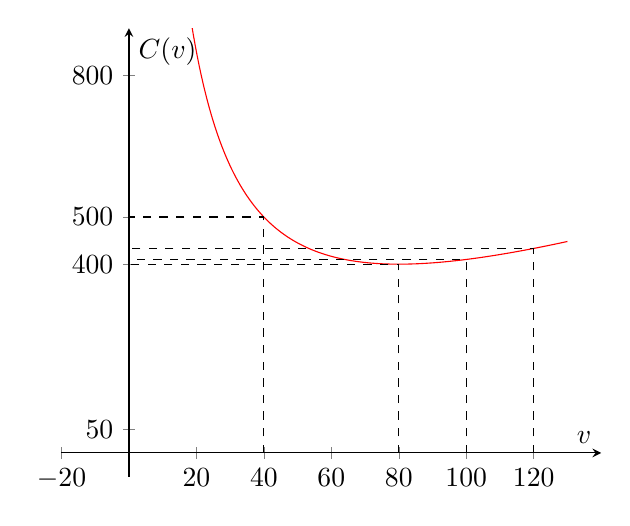
\begin{tikzpicture}
				\begin{axis}[
						 axis x line=middle,
						axis  y line=middle,
						 xlabel={$v$},
						ylabel={$C (v)$}, 
						 xtick={-20,0,20,40,60,80,100,120},
						 ytick={0,50,400,500,800},
						 ymin=-50,ymax=900,
						xmin=-20,xmax=140, 
						domain=10:130, 
						samples=200] 
					 \addplot[color=red] {16000/x + 5/2*x};
					\draw[dashed] (axis cs:120,0)  -- (axis cs:120,433)-- (axis cs:0,433);
					\draw[dashed] (axis cs:80,0)  -- (axis cs:80,400) -- (axis cs:0,400);
					\draw[dashed] (axis cs:40,0) -- (axis cs:40,500) --  (axis cs:0,500);
					\draw[dashed] (axis cs:100,0)  -- (axis cs:100,410) -- (axis cs:0,410);
				\end{axis}
			\end{tikzpicture}
		\end{center}
		Quan sát đồ thị hàm số, ta nhận thấy hàm số đạt GTNN khi $v=80$ và  GTNN là $400$.\\
	Như vậy, để tiết kiệm tiền xăng  nhất, tài xế nên chạy xe với tốc độ trung bình là $80$ km/h.}
\end{bt}

% nguồn: Phan2_Lop_12_Dai_so_Chuong_1
\begin{bt}%[2D1V5-8]%[ma:257ace15]
	Một cầu thủ thực hiện cú sút bóng xoáy (banana kick), làm bóng bay  theo đường cong hình bậc ba thay vì một parabol thông thường. Quỹ đạo bóng trong hệ trục tọa độ $ Oxy $ được mô tả bởi phương trình $ y=\dfrac{x^{3}}{100}-\dfrac{x^{2}}{10}+\dfrac{253 x}{100} $, với $ y $ là độ cao của bóng $ (m) $. Biết chiều cao chuẩn của khung thành là $2{,}44$ m . Khi bóng chạm xà ngang thì góc lệch của bóng và mặt đất là bao nhiêu biết góc lệch của bóng và mặt đất là góc của đường tiếp tuyến với đồ thị hàm số $ y=\dfrac{x^{3}}{100}-\dfrac{x^{2}}{10}+\dfrac{253 x}{100} $ tại điểm chạm xà ngang và trục $ Ox $ (kết quả làm tròn đến hàng đơn vị).
	\shortans{67} 
	 \loigiai{
		Ta có bóng chạm xà ngang  nên ta có tung độ $ y=2{,}44 $ nên
		\[ 
		2{,}44=\dfrac{x^{3}}{100}-\dfrac{x^{2}}{10}+\dfrac{253 x}{100}  \Leftrightarrow x^{3}-10 x^{2}+253 x-244=0 \Leftrightarrow x=1.
		 \]
		Hệ số góc của tiếp tuyến là $  k=f'(1)=\dfrac{3}{100}-\dfrac{1}{5}+\dfrac{253}{100}=\dfrac{59}{25} $.\\
		Gọi $ \alpha $ là góc của tiếp tuyến với  trục $ Ox $, ta có $ \tan \alpha=\dfrac{59}{25} \Rightarrow \alpha \approx 67^{\circ} $.\\
		Vậy góc lệch của bóng và mặt  đất là $67^\circ$.
	 }
\end{bt}

% nguồn: Phan2_Lop_12_Dai_so_Chuong_1
\begin{bt}%[2D1V5-8]%[ma:ff673ee2]
	Một con cá bơi ngược dòng để vượt khoảng cách $250$ km. Vận tốc dòng nước là $5$ km/h. Nếu vận tốc bơi của cá khi nước đứng yên là $v$ (km/h) thì năng lượng tiêu hao của cá trong $t$ giờ được cho bởi công thức $E(v) = cv^3t$, trong đó $c$ là một hằng số và năng lượng $E$ tính bằng Jun.  Khi vận tốc bơi của cá nằm trong khoảng $(m;n)$ lớn nhất ($m$, $n$ là số nguyên hoặc là phân số tối giản) thì năng lượng tiêu hao của cá giảm. Tính $m + 2n$.
	\shortans{20} 
	 \loigiai{
		Vận tốc của cá khi bơi ngược dòng nước là $v - 5$ (km/h). Điều kiện:  $v > 5$.\\
		Thời gian để cá vượt qua quãng đường $250$ km là $t = \dfrac{250}{v -  5}$ (giờ).\\
		Năng lượng tiêu hao của cá để vượt qua quãng đường  đó là $E(v) = cv^3 \cdot \dfrac{250}{v - 5}$ (Jun).\\
		Ta có $E'(v) = 250c \cdot \dfrac{2v^3 - 15v^2}{(v - 5)^2}$. Do đó $E'(v) = 0  \Leftrightarrow \hoac{&v = 0 \text{ (loại)}\\ &v = \dfrac{15}{2}.}$\\
		 Bảng biến thiên
		\begin{center}
			
\begin{tikzpicture}
				 \tkzTabInit[nocadre=false,lgt=1.2,espcl=4,deltacl=0.5]
					{$v$/1,$E'(v)$/1,$E  (v)$/2}
					{$5$,$\dfrac{15}{2}$,$+\infty$} 
				\tkzTabLine{,-,0,+,} 
				 \tkzTabVar{+/$+\infty$,-/$\dfrac{84\,375c}{2}$,+/$+\infty$}
			\end{tikzpicture}
		\end{center}
		Khi đó, vận tốc bơi của cá nằm trong khoảng $\left(5; \dfrac{15}{2} \right)$ thì  năng lượng tiêu hao của cá giảm.\\
		 Do đó $m = 5$, $n = \dfrac{15}{2} \Rightarrow m + 2n = 5 + 15 = 20$.
	} 
\end{bt}

% nguồn: Phan2_Lop_12_Dai_so_Chuong_1
\begin{bt}%[2D1V5-8]%[ma:2580c458]
	Lát cắt của một vùng đất được mô hình hóa là một phần hàm số bậc ba $y=f(x)$ có đồ thị như hình vẽ (đơn vị độ dài trên các trục là kilomét). Biết khoảng cách hai  bên chân đồi $OM=2$\,(km), độ rộng của hồ nước $MN=1$\,(km) và ngọn đồi cao $528$\,(m). Độ sâu nhất của hồ nước là bao~nhiêu mét? (làm tròn kết quả đến hàng đơn vị của mét).
	\shortans{158} 
	 \loigiai{
		 Đổi $528$\,m$= 0{,}528$\,km.\\
		Ta  có: $ON=OM+MN=3$ km $\Rightarrow M(2;0)$, $N(3;0)$.\\
		 Từ đồ thị hàm số suy ra\\
		$\begin{aligned}
		 &f(x)=kx(x-2)(x-3)=k\left(x^3-5x^2+6x\right)\\
		\Rightarrow  &f'(x)=k\left(3x^2-10x+6\right).
	\end{aligned}$\\
	$f’(x)=0\Leftrightarrow  3x^2-10x+6=0\Leftrightarrow\hoac{&x=\dfrac{5+\sqrt{7}}{3}\\&x=\dfrac{5-\sqrt{7}}{3}.}$ \\
	Gọi $h$ với  $(h>0)$ là độ sâu của hồ.\\
	Khi đó $\left(\dfrac{5-\sqrt{7}}{3};0,528\right)$ là đỉnh đồi,  $\left(\dfrac{5+\sqrt{7}}{3};-h\right)$ là đáy hồ.\\
	Ta có  $$k\left[\left(\dfrac{5-\sqrt{7}}{3}\right)^3-5\left(\dfrac{5-\sqrt{7}}{3}\right)^2+6\left(\dfrac{5-\sqrt{7}}{3}\right)\right]=0,528\Leftrightarrow k\approx 0{,}25.$$
	\begin{center}
		\resizebox{!}{5cm}{\begin{tikzpicture}[line join=round,line cap=round,>=stealth]
		 \def\xmin{-.5}\def\xmax{4}\def\ymin{-2}\def\ymax{6}
		\draw[->]  (\xmin-0.2,0)--(\xmax+0.2,0) node[below]{$x$};
		 \draw[->] (0,\ymin-0.2)--(0,\ymax+0.2) node[right]{$y$};
		 \draw (0,0) node[below left]{$O$};
		 \draw (2,0) node[below left]{\footnotesize$M$};
		\draw (3,0) node[below right]{\footnotesize$N$}; 
		\foreach \x in {}\draw (\x,0.1)--(\x,-0.1) node[below]{$\x$}; 
		\foreach \y in {}\draw  (0.1,\y)--(-0.1,\y) node[left]{$\y$};
		 \clip (\xmin,\ymin) rectangle (\xmax,\ymax);
		\draw[smooth,samples=100,domain=\xmin:\xmax] plot  (\x,{1*((\x)^3)+-5*((\x)^2)+6*(\x)+0});
		 \draw[pattern=north west lines,opacity=0.7] plot[domain=0:3.8](\x,{1*((\x)^3)+-5*((\x)^2)+6*(\x)+0})--plot[domain=3.8:0](\x,{0});
		 \draw (3.8,0)--(3.8,5.4);
		\draw  (1,2) node[above]{\footnotesize Đồi};
		\draw (2.5,0)  node[above]{\footnotesize Hồ};
		 \draw (3.5,2.7) node[above left]{\footnotesize Núi};
	\end{tikzpicture}
		} 
	\end{center}
	 Do đó,
	\begin{eqnarray*}
		&  &f(x)=0,25\left(x^3-5x^2+6x\right)\\
		&\Rightarrow&-h=\left[\left(\dfrac{5+\sqrt{7}}{3}\right)^3-5\left(\dfrac{5+\sqrt{7}}{3}\right)^2+6\left(\dfrac{5+\sqrt{7}}{3}\right)\right]\\ 
		&\Leftrightarrow& h\approx  0,15778\,km.
	\end{eqnarray*}
Vậy $h\approx  158$\,m.}
\end{bt}

% nguồn: Phan2_Lop_12_Dai_so_Chuong_1
\begin{bt}%[2D1V5-8]%[ma:f9fe4aeb]
	\immini{Ở một vịnh biển, ngoài xa có một hòn đảo nhỏ. Người ta tiến hành lấn biển để xây một  khu đô thị và làm một tuyến cáp treo nối khu đô thị với hòn đảo để phát triển du lịch. Xét trong hệ tọa độ $ Oxy $ với đơn vị đo tương ứng 1 km có hòn đảo ở $ O $ thì đương bao của phần đất lấn biển có dạng là một phần của đồ thị hàm số $ y=\dfrac{x^{2}+1}{x} $. Giả sử tuyến cáp treo được thiết kế nối đảo với đường bao của khu đô thị với độ dài ngắn nhất. Độ dài của tuyến cáp treo là bao nhiêu km (làm tròn kết quả đến hàng phần mười)?}
	{\begin{tikzpicture}[line cap=round,line join=round]
		\path[draw,fill] (2.33,1.05) -- (3.74,3.49) coordinate (A) circle (1.5pt); 
		\path[draw,fill=white] (0,0).. controls +(35:1.5) and +(90:3.5).. (3.5,0) -- (5,0)  -- (5,-1.5) -- (-2,-1.5) -- (-2,0) -- cycle;
		\fill[draw,pattern=bricks] (-2,-1.5) rectangle (5,-1); 
		\draw (A) node[right]{$O$} circle  (4pt)
			(1.99,.5) node{Khu đô thị}; 
		\draw  (1,-.5) node{Biển};
	\end{tikzpicture}
	 }
	 \shortans{2,2}
	\loigiai{ 
		Độ dài ngắn nhất của tuyến cáp treo nối với đường bao của khu đô thị chính là khoảng cách  từ $ O $ tới điểm cực đại của đồ thị hàm số $ y=\dfrac{x^{2}+1}{x} $.\\
		Xét hàm số $ y=\dfrac{x^{2}+1}{x} $ với  $ x \neq 0 $.\\
		Ta có $ y'=\dfrac{x^{2}-1}{x^{2}}=0  \Rightarrow\hoac{&x=1\\&x=-1.} $\\
		Bảng biến thiên 
		\begin{center}
			
\begin{tikzpicture}
				\tkzTabInit[lgt=1.2,espcl=2.5] 
					 {$x$/1,$y'$/1,$y$/2}
					{$-\infty$,$-1$,$0$,$1$,$+\infty$} 
				 \tkzTabLine{,+,z,-,d,-,z,+,}
				\tkzTabVar{-/ $-\infty$,+/ $-2$,-D+ / $-\infty$ / $+\infty$,-/ $2$,+/ $+\infty$} 
			\end{tikzpicture}
		\end{center}
		Dựa vào bảng biến thiên, đồ thị hàm số có  điểm cực đại là $ A(-1;-2) $.\\
		Khi đó $  OA=\sqrt{(-1)^{2}+(-2)^{2}}=\sqrt{5} \approx 2{,}2 $.\\
		Vậy độ dài của tuyến cáp treo xấp xỉ $ 2{,}2$  km.
	 }
\end{bt}

% nguồn: Phan2_Lop_12_Dai_so_Chuong_1
\begin{bt}%[2D1V5-8]%[ma:618e7612]
	Mỗi tuần, một cửa hàng bán điện thoại di động trung bình bán được $1\,000$ điện thoại A với giá $14$ triệu đồng một cái. Biết rằng, nếu cứ giảm giá bán $500$  nghìn đồng/ $1$ cái, số lượng điện thoại A bán ra sẽ tăng thêm khoảng $100$ cái mỗi tuần. Biết rằng nếu bán $x$ cái điện thoại A thì giá mỗi cái là $p(x)$ (triệu đồng) và hàm chi phí hàng tuần $C(x)=12\,000-3x$ (triệu đồng). Để lợi nhuận là lớn nhất, cửa hàng nên bán mỗi cái điện thoại A với giá bao nhiêu (triệu đồng)?
	 \shortans{8}
	\loigiai{Theo  giả thiết $p(x)=ax+b$, $\left(\forall x >0\right)$.\\
		Do đó, phương trình đường thẳng $p(x)=ax+b$ đi qua hai điểm $(1\, 000;14)$ và $(1\,100;13{,}5)$ nên  ta có hệ phương trình
		 \[\heva{&14=1\,000a+b\\&13{,}5=1\,100a+b}\Leftrightarrow\heva{&a=-\dfrac{1}{200}\\&b=19.}\]
		Suy ra $p(x)=-\dfrac{1}{200}x+19$. \\ 
		Doanh  thu bán hàng của $x$ sản phẩm là $R(x)=x \cdot \left(-\dfrac{1}{200}x+19\right) =-\dfrac{x^{2}}{200}+19x$ (triệu đồng).\\
		Do đó, hàm số thể hiện lợi nhuận thu được sau khi bán $x$ sản phẩm là 
		\[P(x)=R(x)-C(x) 
		=-\dfrac{x^{2}}{200}+19x-12\,000+3x 
		 =-\dfrac{x^{2}}{200}+22x-12\,000 \ \text{ (triệu đồng)}.\]
		 Ta có $P'(x)=-\dfrac{x}{100}+22$.\\
		Suy ra $P'(x)=0  \Leftrightarrow x=2\,200$.
		\begin{center}
			\begin{tikzpicture}
				 \tkzTabInit [lgt=1.5,espcl=3,nocadre]
					{$x$/0.8,$P'(x)$/0.8,$P  (x)$/2}
					 {$-\infty$,$0$,$2\,200$,$+\infty$}
				 \pattern[pattern=north west lines] (T11) rectangle (N23);
				\draw[teal,double,shift={(0.5,0)}](N21)--(N23); 
				\tkzTabLine  {,,d,+,0,-,}
				\node[above right]  (0) at (N23) {$-\infty$};
				\node[below]  (1) at (N32) {$24\,400\,000$};
				 \node[above] (3) at (N43) {$-\infty$};
				 \draw[teal,->] (0)--(1);
				\draw[teal,->]  (1)--(3);
			\end{tikzpicture}
		\end{center}
		Ta thấy bán $2\,200$ cái điện thoại A thì lợi nhuận đạt  cao nhất.\\
	Vậy cửa hàng nên đặt giá bán là $p(2\,200)=8$ (triệu  đồng).}
\end{bt}

% nguồn: Phan2_Lop_12_Dai_so_Chuong_1
\begin{bt}%[2D1V5-8]%[ma:e3c33b31]
	Một con cá hồi bơi ngược dòng nước để vượt một khoảng cách là $300$ km. Vận tốc dòng nước là $6$ (km/h). Nếu vận tốc bơi của cá khi nước đứng yên là $v$ (km/h) thì năng lượng tiêu hao của cá trong $t$ giờ được cho bởi công thức $E(v)=cv^3t$ (trong đó $c$ là hằng số dương, $E$ được tính bằng đơn vị Jun). Cá bơi ngược dòng quãng đường $300$ km trên trong khoảng thời gian  $t$ với vận tốc bằng bao nhiêu để năng lượng tiêu hao là thấp nhất?
	 \shortans{9}
	 \loigiai{
		Vận tốc khi  cá bơi ngược dòng sẽ là $v-6$ (km/h).\\
		Thời gian để bơi quãng  đường $300$km là $t=\dfrac{300}{v-6}(h)$.\\
		Năng lượng tiêu hao là $E(v)=300c\dfrac{v^3}{v-6}$(J) .\\ 
		Do  $c>0\Rightarrow E{(v)_{\min}}\Leftrightarrow\dfrac{v^3}{v-6}=\left(f(v)\right)_{\min}$ .\\
		Với $v > 6$ ta có $f'(v)=\dfrac{3v^2\left(v-6\right)-v^3}{\left(v-6\right)^2}=\dfrac{2v^3-18v}{\left(v-6\right)^2}=0\Leftrightarrow\left[\begin{array}{*{20}{l}}
		{v=0}\\ 
		{v=9.} 
	\end{array}\right.$\\
	Bảng  biến thiên
	\begin{center}
		
\begin{tikzpicture}
			 \tkzTabInit[nocadre=false,espcl=2.5,lgt=1.2,deltacl=0.6]
				{$v$/0.6,$f'(v)$/0.6,$f (v)$/2} 
				{$6$,$9$,$+\infty$} 
			\tkzTabLine{,-,0,+,} 
			 \tkzTabVar{+/$+\infty$,-/$f_{\min}$,+/$+\infty$}
		\end{tikzpicture}
	\end{center}
Vậy để năng lượng tiêu hao là thấp nhất  thì vận tốc là $9$ (km/h).}
\end{bt}

% nguồn: Phan2_Lop_12_Dai_so_Chuong_1
\begin{bt}%[2D1V5-8]%[ma:60e2ca13]
	Một máy bay trình diễn có đường bay gắn với hệ trục $ Oxy $ được mô phỏng như hình vẽ, trục $ Ox $ gắn với mặt đất. 
	\begin{center}
		\begin{tikzpicture}[scale=0.8]
			\clip (-1,-2) rectangle  (11,6);
			\begin{scope}[->]
				\draw (-6,0) -- (11,0) node[right] {$x$}; 
				\draw (0,-6) --  (0,6) node[above] {$y$};
			\end{scope}
			\begin{scope}[domain=-6:1.9,smooth,samples=400]
				\draw[blue] plot  (\x,{-\x + 10.5 - 4/(\x-2)});
			\end{scope}
			\begin{scope}[domain=2.1:11,smooth,samples=400]
				\draw plot (\x,{-\x + 10.5  - 4/(\x-2)});
			\end{scope}
			\begin{scope}[dashed]
				\draw (2,-6) -- (2,6) node[above  left] {$x=2$};
			\end{scope}
			\begin{scope}[dashed,domain=-6:11]
				\draw plot  (\x,{-\x+10.5}) node[below right] {$y=-x+\tfrac{21}{2}$};
			\end{scope}
			\fill (2.5,0) circle (2pt) node[below right] {$A$}; 
			\fill (10,0) circle  (2pt) node[below] {$C$};
			\fill (10.5,0) circle (2pt) node[above right] {$G$}; 
			\fill (4,4.5) circle (2pt) node[above] {$B$}; 
		\end{tikzpicture}
	\end{center}
	Đường bay có dạng là một phần của đồ thị hàm phân thức bậc hai trên bậc nhất $ y=f(x) $ có đường tiệm cận đứng là $ x=2 $. Điểm $ G $ là giao  điểm của đường tiệm cận xiên của đồ thị hàm số $ y=f(x) $ và trục $ Ox $ được gọi là điểm giới hạn. Biết máy bay bay từ vị trí $ A $ cách tọa tọa độ $ O $ một khoảng $2{,}5$ đơn vị và máy bay khi ở vị trí cao nhất cách điểm xuất phát $1{,}5$ đơn vị theo phương song song với trục $ Ox $ và cách mặt đất $4{,}5$ đơn vị. Vị trí máy bay tiếp đất cách điểm giới hạn một khoảng bằng bao nhiêu?
	 \shortans{0,5}
	 \loigiai{
		Vì tiệm cận đứng của đồ thị hàm số $ y=f(x) $ (hàm phân thức bậc hai  trên bậc nhất) là $ x=2 $.
		 Hàm số có dạng $ y=f(x)=ax+b+\dfrac{c}{x-2}$, $(a<0)$.\\
		Đồ thị hàm số  qua điểm $ A\left(\dfrac{5}{2}; 0\right) $ và nhận $ B\left(4; \dfrac{9}{2}\right) $ làm điểm cực trị, suy ra
		\[ 
		 \heva{
		& \dfrac{5}{2}a + b + 2c =  0 \\
		& 4a + b  + \dfrac{1}{2}c = \dfrac{9}{2} \\
		&  a - \dfrac{1}{4}c = 0
		} 
		\Rightarrow \heva{ 
		& a=-1 \\ 
		& b=\dfrac{21}{2} \\ 
		& c=-4. 
		} 
		\] 
		Khi đó $  f(x)=-x+\dfrac{21}{2}-\dfrac{4}{x-2} $.\\
		Đồ thị hàm số có tiệm cận xiên $ y=-x+\dfrac{21}{2} $. Tọa độ điểm $ G\left(\dfrac{21}{2}; 0\right) $.\\ 
		Phương trình  cho hoành độ giao điểm của đồ thị hàm số $ y=f(x) $ với trục $ Ox $ là
		 \[
		-x+\dfrac{21}{2}-\dfrac{4}{x-2}=0 \Rightarrow-x^{2}+\dfrac{25}{2}  x-25=0 \Leftrightarrow\hoac{&x=\dfrac{5}{2} \\&
		x=10}\Rightarrow C(10; 0). 
		\] 
		 Do đó $CG=\dfrac{21}{2}-10=\dfrac{1}{2}=0{,}5$.
	 }
\end{bt}

% nguồn: Phan2_Lop_12_Dai_so_Chuong_1
\begin{bt}%[2D1V5-8]%[ma:9a113e5b]
	Vì nước và dầu không hoà tan  vào nhau nên nếu dầu đổ vào nước sẽ tạo thành một mảng hình trụ trên bề mặt nước. Bán kính $r(t)$ của mảng này lan ra với tốc độ tỉ lệ thuận với chiều cao $h(t)$ của mảng dầu. Giả sử một lít dầu bị đổ trên mặt hồ tĩnh lặng. Bán kính ban đầu của vết tràn là $20$ cm và sau $2$ giây nó tăng lên $50$ cm. Hỏi sau bao nhiêu phút (làm tròn đến hàng phần mười) thì bán kính vết tràn đạt $5$ mét? \shortans{35,6}
	\loigiai{ 
		Vì mảng dầu này lan có dạng hình trụ, nên ta có thể tích  khối dầu \[V=\pi \cdot r^2(t) \cdot h(t)\Leftrightarrow h(t)=\dfrac{V}{\pi r^2(t)}.\]
		Bán kính $r(t)$ của mảng dầu  lan ra với tốc độ $r'(t)$, mà tốc độ lan ra $r'(t)$ tỉ lệ thuận với chiều cao $h(t)$ của mảng dầu nên theo tính chất của hai đại lượng tỉ lệ thuận.\\
		Ta  có $r'(t)=k \cdot h(t)$\qquad $(*)$.\\
		Thay $h(t)=\dfrac{V}{\pi r^2(t)}$ vào biểu  thức (*), ta được $r'(t)=k \dfrac{V}{\pi r^2(t)}$.\\
		Vì $k \dfrac{V}{\pi}$ là  $1$ đại lượng không đổi nên đặt $k \dfrac{V}{\pi}=a$.\\
		Khi đó 
		\[r'(t)=k \dfrac{V}{\pi r^2(t)} \Leftrightarrow r'(t)=\dfrac{a}{r^2(t)} \Leftrightarrow 3r'(t) \cdot r^2(t)=3a  \Leftrightarrow\left[r^3(t)\right]'=3a.\]
		Nguyên hàm $2$ vế, ta được $r^3(t)=\displaystyle\int 3a \mathrm{\,d}t \Leftrightarrow  r^3(t)=3at+C$.\\
		Vì bán  kính ban đầu của vết tràn là $20$ cm và sau $2$ giây nó tăng lên $50$ cm, ta có hệ phương trình \allowdisplaybreaks
		\begin{eqnarray*}
			&&\heva{& r(0)=20\\ &  r(2)=50}\\
			&\Leftrightarrow&\heva{&C=20^3=8\,000  \\ & 3\cdot2a+C=50^3}\\
			&\Leftrightarrow&\heva{&C=8\,000\\ &a=19\,500.} 
		\end{eqnarray*}
		Do đó $r^3(t)=58\,500t+8\,000$  cm.
		Đổi $5\,\mathrm{m}=500\,\mathrm{cm}$.\\ 
		Bán  kính vết tràn đạt $4$ m tương đương với \allowdisplaybreaks
		\[r(t)=500\Leftrightarrow 500^3=58\,500t+8\,000\Leftrightarrow t=\dfrac{500^3-8\,000}{58\,500} \approx  2\,136{,}61.\]
		Vậy thời gian bán kính vết tràn đạt $5$ mét là khoảng  $2\,136{,}61$ giây và bằng $35{,}6$ phút.
	 }
\end{bt}

% nguồn: Phan2_Lop_12_Dai_so_Chuong_1
\begin{bt}%[2D1V5-8]%[ma:88951c54]
	Khuôn viên của một công viên có dạng hình chữ nhật $A B C D$ với $A B=100 \mathrm{~m}; A D=80 \mathrm{~m}$. Người ta muốn chia công viên thành hai khu, một khu dành cho trẻ em, một khu dành cho người lớn. Để tạo thiết kế độc đáo và lạ mắt, người ta dùng một đường cong chia khuôn viên thành hai phần $H_1$ (không tô màu) dành cho trẻ em và $H_2$ (tô màu) dành cho người lớn như hình vẽ bên với $A H=40 \mathrm{~m}; A E=60 \mathrm{~m}; A P=20 \mathrm{~m}$  và $E F / / A B; P Q / / A D$.
	Biết rằng khi xét trong một hệ tọa độ $Oxy$, đường cong trong hình là một phần của đồ thị hàm số bậc ba. Phần chính giữa công viên người ta muốn mắc dây đèn trang trí dọc đoạn thẳng $M N$ như hình. Biết giá tiền mỗi mét dây trang  trí của phần dành cho trẻ em là 140 nghìn đồng và phần dành cho người lớn là 180 nghìn đồng. Tổng số tiền mắc dây đèn trang trí trên đoạn $M N$ là bao nhiêu triệu đồng.
	\begin{center}
		\begin{tikzpicture}[scale=0.5,>=stealth,x=1cm,y=1cm,font=\footnotesize,line join=round,line cap=round]
			\def\f (\x){(0.05*(\x)^3-0.7*(\x)^2+2.2*(\x)+4)} 
			\fill[pattern=crosshatch dots,smooth] (0,0)  --
				plot[domain=0:10]  (\x,{\f (\x)})
				-- (10,0)  -- cycle;
			\draw[smooth,red,line  width=1]
				plot[domain=0:10] (\x,{\f  (\x)});
			\draw (2,0) node[below]{$P$} 
				 (10,0) node[below]{$B$}
				(0,4) node[left]{$H$} 
				 (0,6) node[left]{$E$}
				(0,8) node[left]{$D$} 
				 (10,6) node[right]{$F$}
				 (10,8) node[right]{$C$}
				(5,8) node[above]{$N$} 
				(2,6) node[above]{$Q$}; 
			\draw[line  width=1pt]((0,0)--(10,0)--(10,8)--(0,8)--(0,0);
			 \draw[dashed] (0,6)--(10,6);
			\draw[red] (5,0) node[below]{$M$}--(5,3.75)  node[right]{$I$} -- (5,8) node[above]{$N$};
		\end{tikzpicture}
	\end{center}
	\shortans{12,7} 
	\loigiai{ 
		\begin{center}
			\begin{tikzpicture}[scale=0.5,>=stealth,x=1cm,y=1cm,font=\footnotesize,line join=round,line cap=round]
				\def\f (\x){(0.05*(\x)^3-0.7*(\x)^2+2.2*(\x)+4)} 
				\draw[->]  (-0.5,0)--(0,0) node[below
					 left]{$O$}--(11,0)
					node[above]{$x$}; 
				\draw[->]  (0,-0.5)--(0,9)
					 node[left]{$y$};
				 \fill[pattern=crosshatch dots,smooth] (0,0) --
					plot[domain=0:10]  (\x,{\f (\x)})
					-- (10,0)  -- cycle;
				 \draw[smooth,red,line width=1]
					 plot[domain=0:10] (\x,{\f (\x)});
				 \draw (2,0) node[below]{$P$}
					(10,0)  node[below]{$B$}
					 (0,4) node[left]{$H$}
					 (0,6) node[left]{$E$}
					(0,8)  node[left]{$D$}
					 (10,6) node[right]{$F$}
					(10,8)  node[right]{$C$}
					 (5,8) node[above]{$N$}
					 (2,6) node[above]{$Q$}
					(5,0) node[below]{$M$} 
					 (5,3.75) node[right]{$I$};
				\draw[line width=1pt](0,8)--(10,8)--(10,0); 
				\draw[dashed] (5,0)--(5,8) 
					 (0,6)--(10,6)
					 (2,0)--(2,6);
			\end{tikzpicture}
		\end{center}
		Xét trục tọa độ $Oxy$, với gốc tọa độ là điểm $A$. Tia $Ox$ trùng với tia $A B$, tia $O y$ trùng với tia $A D$ thì đường cong ranh giới giữa hai  khu vực là đồ thị hàm số bậc ba $y=a x^3+b x^2+c x+d$.
		Theo giả thiết đồ thị  hàm số này đi qua các điểm $H(0; 40); Q(20; 60); F(100; 60)$ và có điểm cực trị là $Q(20; 60)$ nên ta có hệ
		 $$
		\left\{\begin{array}{l}
		d=40  \\
		60=8000 a+400 b+20 c+d  \\
		60=1000000 a+10000 b+100 c+d \\ 
		1200 a+40  b+c=0
	\end{array}\right.
	 $$
	Giải hệ  trên ta được $a=\dfrac{1}{2000}; b=\dfrac{-7}{100}; c=\dfrac{11}{5}; d=40$.
	Do $M$ là trung điểm của $A B$ nên tọa độ điểm $I$ là $(50; 37,5)$. Do đó chiều dài đoạn dây  thuộc phần dành cho người lớn là $37,5 \mathrm{~m}$, chiều dài đoạn dây thuộc phần dành cho trẻ em là $42,5 \mathrm{~m}$.\\
	Tổng  số tiền mắc dây đèn là $37,5 \cdot 0,18+42,5 \cdot 0,14=12,7$ (triệu đồng).
	 }
	\end{bt}

% nguồn: Phan2_Lop_12_Dai_so_Chuong_1
\begin{bt}%[2D1V5-8]%[ma:8a9fff2f]
		Ông An đang ở trong rừng để đào vàng. Ông ta tìm thấy vàng ở điểm $X$, cách điểm $A$ $3$ km. Điểm $A$ nằm trên đường bờ biển (đường bờ biển là đường thẳng). Trại của ông An nằm ở $Y$, cách điểm $B$ $3$ km. Điểm $B$ cũng thuộc đường bờ biển. Biết rằng $AB=18$  km, $AM=NB=x$ km và $AX=BY=3$ km. (như hình vẽ)
		\begin{center}
			\begin{tikzpicture}>=stealth,line join=round,line cap=round]
				 \path (1,0) coordinate (A)
					 (3,0) coordinate (M)
					(6,0) coordinate  (N)
					(8,0)  coordinate (B)
					(1,2) coordinate (X) 
					(8,2) coordinate (Y); 
				\draw (0,0)--(A)--(M) node[below,pos=0.5]{$x$ km}--(N) node[below,pos=0.5]{\textbf{Bờ biển}} --(B) node[below,pos=0.5]{$x$  km}--(9,0)
					(A)--(X) 
					 (B)--(Y)
					(4.5,1)  node[above]{\textbf{RỪNG}}
					(X)  node[above]{Vàng}
					(Y) node[above]{Trại của Ông  An};
				 \draw[dashed,->] (X)--(M);
				\draw[dashed,->]  (Y)--(N);
				\draw[<->] (0,-1)--(9,-1) node[below,pos=0.5]{$18$  km};
				\foreach \p/\g  in {A/-90,B/-90,M/-90,N/-90,B/-90,X/190,Y/-10}
				\draw (\p) circle  (1pt) node[shift=(\g:3mm)] {$\p$};
			\end{tikzpicture}
		\end{center}
		Khi đang đào vàng, ông An bị rắn cắn, chất độc lan vào máu. Sau khi bị cắn, nồng độ chất độc trong máu tăng theo thời gian được tính theo hàm số $y=50\log\left(t+2\right)$ (mg/l), trong đó $y$ là nồng độ, $t$ là thời gian tính bằng giờ sau khi bị rắn cắn. Ông An cần quay trở lại trại để lấy thuốc giải độc. Ông ấy chạy trong rừng với vận tốc $5$ km/h và chạy trên đường bờ biển với vận tốc $13$ km/h. Để về đến trại ông An cần chạy từ trong rừng qua điểm $M$, $N$ trên đường bờ biển. Chọn điểm $M$ trên đường bờ biển sao cho khi ông An về đến trại nồng độ chất độc trong máu thấp nhất. Tính nồng  độ chất độc trong máu thấp nhất khi ông An về đến trại (làm tròn đáp án đến hàng phần chục).
	 \shortans{32,6}
	\loigiai{ 
		Nồng độ chất độc trong máu thấp nhất khi thời gian di chuyển về  đến trại thấp nhất.\\
		Vậy nên quãng  đường ông An di chuyển về đến trại phải ngắn nhất.\\
		 Theo bài ra ta có ông An sẽ đi quãng đường $XM+MN+NY$.\\
		Ta  có $XM=NY=\sqrt{9+x^2}$; $MN=18-2x$ (km).\\
		 Thời gian ông An chạy đến trại nghỉ là $T(x)=2\left(\dfrac{\sqrt{9+x^2}}{5}+\dfrac{9-x}{13} \right)$ với $\left[0;9\right]$.\\
		Xét $T'(x)=2\left(\dfrac{x}{5\sqrt{9+x^2}}-\dfrac{1}{13} \right)$.\\ $T'(x)=0\Rightarrow x=\dfrac{5}{4}$ (thỏa  mãn).\\
		Bảng  biến thiên
		\begin{center}
			\begin{tikzpicture}[font=\normalsize,t style/.style={style=solid}]
				 \tkzTabInit[nocadre,lgt=1.2,espcl=2.5,deltacl=0.5]
					{$x$/0.75,$T'(x)$/0.75,$T (x)$/3} 
					{$0$,$\tfrac{5}{4}$,$9$} 
				 \tkzTabLine{,-,0,+}
				\path 
					($(N13)!0.8!(N12)$) node  (A1){$ \tfrac{168}{65} $}
					($(N23)!0.1!(N22)$) node (A2){$ \tfrac{162}{65}  $}
					 ($(N33)!0.8!(N32)$) node (A3){$ \tfrac{6\sqrt{10}}{5} $};
				\foreach \x/\y in  {A1/A2,A2/A3}{
					\draw[-stealth] (\x)--(\y); 
				 }
			\end{tikzpicture}
		\end{center}
		Dựa vào bảng biến  thiên, ta thấy $T(x)$ nhỏ nhất khi $x=\dfrac{5}{4}$; ${\mathop{\min}\limits_{\left(0;9\right)}} T(x)=T\left(\dfrac{5}{4} \right)=\dfrac{162}{65}$.\\
		Vậy nồng độ  chất độc trong máu thấp nhất là ${\mathop{\min}\limits_{\left(0;+\infty \right)}} y=50\log\left(\dfrac{162}{65}+2\right)\approx 32{,}6$.
	} 
\end{bt}

% nguồn: Phan2_Lop_12_Dai_so_Chuong_1
\begin{bt}%[2D1V5-8]%[ma:639fe2c8]
	Theo định luật làm mát của Newton thì tốc độ làm mát của một vật tỉ lệ thuận với chênh lệch nhiệt độ giữa vật đó và môi trường xung quanh, với điều kiện là chênh lệch này không quá lớn. Giả sử $T(t)$ là nhiệt độ của vật thể (đơn vị: độ C) tại thời điểm $t$ (đơn vị: phút) và $T_s$ là nhiệt độ của môi trường xung quanh, chênh lệch giữa nhiệt độ của vật thể và môi trường xung quanh là $y(t)=T(t)-T_s$ thì $y'(t)=k \cdot y(t)$ với $k$ là hằng số. Một cốc nước đang ở nhiệt độ phòng là $22^{\circ} C$ được đưa vào ngăn mát tủ lạnh có nhiệt độ là $5^{\circ}$C. Sau $30$ phút, nhiệt độ của cốc nước được đo lại là $16^{\circ}$C.  Hỏi sau một tiếng trong tủ lạnh, nhiệt độ cốc nước là bao nhiêu $^\circ$C (kết quả làm tròn đến hàng đơn vị).
	\shortans{12} 
	\loigiai{ 
		Đổi $1$  giờ $=60$ phút.\\
		Yêu cầu bài toán là xác định nhiệt độ  của cốc nước sau $1$ giờ hay $T(60)$.\\
		 Ta có
		\[y'(t)=k \cdot  y(t) \Rightarrow \dfrac{y'(t)}{y(t)}=k \Leftrightarrow[\ln y(t)]'=k.\]
		Nguyên hàm $2$ vế, ta  được
		\[\ln y(t)=\displaystyle\int k \mathrm{\,d}t=k t+C\Rightarrow y(t)=\mathrm{e}^{k  t+C}.\]
		Khi đặt  cốc nước vào tủ lạnh thì khi đó nhiệt độ môi trường xung quanh $T_s=5$.\\
		Khi đó $y(t)=T(t)-T_s$ tương đương với $\mathrm{e}^{k t+C}=T(t)-5\Rightarrow \mathrm{e}^{k  t+C}+5=T(t)$.\\
		Ta có $\mathrm{e}^{k\cdot 0+C}+5=T(0) \Leftrightarrow \mathrm{e}^C+5=22\Leftrightarrow \mathrm{e}^C=17\Leftrightarrow C=\ln  17$.\\
		Suy ra  $T(t)=\mathrm{e}^{k t+\ln 17}+5$.\\
		Biết sau $30$ phút, nhiệt độ của cốc nước là $16^{\circ} C$ nên  ta có \allowdisplaybreaks
		\begin{eqnarray*}
			&&T(30)=16\\ 
			&\Leftrightarrow& \mathrm{e}^{30k+\ln  17}+5=16\\
			 &\Leftrightarrow& \mathrm{e}^{30k+\ln 17}=11\\
			&\Leftrightarrow&  30k+\ln 17=\ln 11\\
			&\Leftrightarrow& 30k=\ln 11-\ln 17=\ln\dfrac{11}{17}\\ 
			&\Leftrightarrow& k=\dfrac{1}{30}  \ln\dfrac{11}{17}.
		\end{eqnarray*}
		Suy ra $T(t)=\mathrm{e}^{\tfrac{1}{30} \ln\tfrac{11}{17} t+\ln  17}+5$.\\
		Vậy nhiệt độ  của cốc nước sau $1$ giờ trong tủ lạnh là $T(60)=\mathrm{e}^{60\cdot \tfrac{1}{30} \ln\tfrac{11}{17}+\ln 17}+5\approx 12^{\circ}$C.
	 }
\end{bt}

% nguồn: Phan2_Lop_12_Dai_so_Chuong_1
\begin{bt}%[2D1V5-8]%[ma:e77f9bc6]
	Vi khuẩn HP (Helicobacter pylori) gây đau dạ dày sau ngày thứ $t\,(t \geq 1)$ với số lượng là $F(t)$ nếu phát hiện sớm thì bệnh nhân sẽ được cứu chữa. Biết rằng $F'(t)=\dfrac{1\,100}{3t}+1$ và sau $1$ ngày bệnh nhân có  $2\,000$ con vi khẩn trong dạ dày. Sau $15$ ngày bệnh nhân phát hiện ra bị bệnh. Hỏi khi đó có bao nhiêu con vi khuẩn trong dạ dày (kết quả làm tròn đến hàng đơn vị)?
	\shortans{3,01} 
	 \loigiai{
		 Ta có $F(t)=\displaystyle\int F'(t)\mathrm{\,d}t=\displaystyle\int\left(\dfrac{1\,100}{3t}+1\right)\mathrm{\,d}t=\dfrac{1\,100}{3} \ln{t}+t+C$.\\
		Có $F(1)=2\,000\Rightarrow 1+C=2\,000\Rightarrow C=1\,999\Rightarrow F(t)=\dfrac{1\,100}{3} \ln{t}+t+1\,999$.\\ 
		Vậy sau $15$  ngày thì số con vi khuẩn trong dạ dày là \[F(15)=\dfrac{1\,100}{3} \ln 15+15+1\,999\approx 3\,007\;\text{ (con).}\]
	} 
\end{bt}

% nguồn: Phan2_Lop_12_Dai_so_Chuong_1
\begin{bt}%[2D1V5-8]%[ma:3b87aeb0]
	Số lượng cá thể của một loài sinh vật phụ thuộc nhiệt độ môi trường sống và được sấp xỉ bởi hàm số $f(t)=300 \cdot e^{\tfrac{t}{5}-\dfrac{3t^2}{100}}$, trong đó $t$ là nhiệt độ môi trường xét từ $0^{\circ}$  đến $60^{\circ}$. Hỏi số cá thể loài sinh vật trên nhiều nhất là bao~nhiêu?
	\shortans{419} 
	 \loigiai{
		Xét hàm số $f(t)=300 \cdot  e^{\tfrac{t}{5}-\dfrac{3t^2}{100}}$. \\
		TXĐ $\mathscr{D} = \mathbb{R}$, $[0; 60]\subset  \mathscr{D}$. \\
		$f'(t)=300 \cdot \left(\dfrac{1}{5}-\dfrac{3t}{50} \right) \cdot e^{\tfrac{t}{5}-\dfrac{3t^2}{100}}$, $f'(t)=0\Leftrightarrow 300 \cdot \left(\dfrac{1}{5}-\dfrac{3t}{50} \right) \cdot e^{\tfrac{t}{5}-\dfrac{3t^2}{100}}=0\Leftrightarrow  t=\dfrac{10}{3} \in \left(0; 60\right)$. \\
		$f(0)=300$; $f\left(\dfrac{10}{3} \right)=300\cdot e^{\tfrac{10}{15}-\dfrac{3\cdot 100}{100\cdot 9}}=300\cdot e^{\tfrac{1}{3}} \approx 419$,  $f(60)=300\cdot e^{\tfrac{60}{5}-\dfrac{3\cdot 60^2}{100}} \approx 6{,}09\cdot 10^{-40}$. \\
		Vậy $\max\limits_{\left[0; 60\right]} f(t)=f\left(\dfrac{10}{3} \right)\approx  419$.
	 }
\end{bt}

% nguồn: Phan2_Lop_12_Dai_so_Chuong_1
\begin{bt}%[2D1V5-8]%[ma:0e609196]
	Sau khi phát hiện một bệnh dịch, các  chuyên gia y tế ước tính số người nhiễm bệnh kể từ ngày xuất hiện bệnh nhân đầu tiên đến ngày thứ $t$ là $N(t)=45t^2-t^3,\;0\leqslant t \leqslant 30$ (người). Nếu xem $N'(t)$ là tốc độ truyền bệnh (người/ngày) tại thời điểm $t$ thì tốc độ truyền bệnh lớn nhất sẽ vào ngày thứ bao nhiêu?
	 \shortans{15}
	\loigiai{ 
		Ta có: $N(t)=45t^2-t^3,0\leq  t \leq 30$;
		 $N'(t)=90t-3t^2$, $N^{\prime \prime}(t)=90-6t$.\\
		$N^{\prime \prime}(t)=0\Leftrightarrow  90-6t=0\Leftrightarrow t=15$.\\
		Bảng  biến thiên:
		\begin{center}
			\begin{tikzpicture}
				 \tkzTabInit[nocadre=true,lgt=1.2,espcl=2.5,deltacl=0.5]{$x$/.7,$N''(t)$/.7,$N'(t)$/2}
					{$0$,$15$,$30$} 
				\tkzTabLine{,+,$0$,-,} 
				 \tkzTabVar{-/$0$,+/$675$,-/$0$}
			\end{tikzpicture}
		\end{center}
		Vậy tốc độ truyền bệnh lớn nhất  sẽ vào ngày thứ $15$.
	 }
\end{bt}

% nguồn: Phan2_Lop_12_Dai_so_Chuong_1
\begin{bt}%[2D1V5-8]%[ma:2bc5ef18]
	Một loại thuốc được dùng cho một bệnh nhân và nồng độ thuốc trong máu của bệnh nhân được giám sát bởi bác sĩ. Biết rằng nồng độ trong máu của bệnh nhân sau khi tiêm vào cơ thể trong $t$ giờ được cho bởi công thức $c(t)=\dfrac{t}{t^2+1}$ (mg/L). Gọi $(a;b)$ là khoảng thời gian nồng độ thuốc trong máu bệnh nhân  tăng. Khi đó, tính $T=a+b$.
	 \shortans{1}
	 \loigiai{
		Ta có $t \ge 0$ và $c'(t)=\dfrac{1-t^2}{(t^2+1)^2}=0\Leftrightarrow\hoac{&t=1\\&t=-1.}$\\ 
		Bảng biến thiên của  hàm số $c(t)$ trên $[0;+\infty)$ là
		\begin{center}
			\begin{tikzpicture}
				 \tkzTabInit[lgt=1.2,espcl=3]
					{$t$ /.7,$c’(t)$ /.7,$c (t)$ /2.5} 
					{$0$,$1$,$+\infty$} 
				 \tkzTabLine{,+,z,-,}
				\tkzTabVar{-/$0$,+/$\dfrac{1}{2}$,-/$0$} 
			\end{tikzpicture}
		\end{center}
		Dựa vào bảng biến thiên thì khoảng thời gian nồng độ trong máu bệnh nhân tăng là $(0;1)$.\\ 
		Suy ra  $a=0$ và $b=1$.\\
		Vậy $T=a+b=0+1=1$. 
	 }
\end{bt}

% nguồn: Phan2_Lop_12_Dai_so_Chuong_1
\begin{bt}%[2D1V5-8]%[ma:f4f0d8bf]
	Một cái cây được gieo trồng từ hạt trong một chiếc chậu. Chiều cao của nó sau $t$ (năm) được cho bởi hàm  số $h(t)$ (đơn vị mét). Tốc độ thay đổi chiều cao của nó sau $t$ (năm) là $h'(t)=0{,}2t+0{,}15$ (mét/năm) với $(0\leq t \leq 4)$. Sau khi trồng được $4$ năm, cây được lấy ra khỏi chậu và trồng xuống đất, chiều cao của nó theo thời gian khi này thay đổi với tốc độ $h'(t)=\dfrac{11}{t}\;(t \geq 4)$. Hỏi sau $4$ năm trồng xuống đất cây cao bao nhiêu mét (\textit{kết quả làm tròn đến hàng phần mười})?
	\shortans{9,8} 
	\loigiai{ 
		\textbf{Bước 1:} Tính chiều cao của cây sau $4$ năm đầu (trong chậu).\\ 
		Để tìm  $h(t)$, ta lấy nguyên hàm của $h'(t)$.\\
		 Ta có $h(t)=\displaystyle\int(0{,}2t+0{,}15)\mathrm{\,d}t=0{,}2\cdot\dfrac{t^2}{2}+0,15t+C=0{,}1t^2+0{,}15t+C$.\\
		 Vì cây gieo từ hạt, chiều cao ban đầu tại $t=0$ là $h(0)=0$.\\
		Ta có $h(0)=0,1(0)^2+0,15(0)+C=0\Rightarrow C=0$.\\ 
		Vậy $h(t)=0{,}1t^2+0{,}15t$.\\ 
		Chiều cao của cây sau $4$ năm (khi lấy ra khỏi chậu) là  $h(4)$\\
		$h(4)=0{,}1\cdot(4)^2+0{,}15\cdot 4=0{,}1\cdot  16+0{,}6=1{,}6+0{,}6=2{,}2$ (mét).\\
		\textbf{Bước 2:} Tính  chiều cao tăng thêm của cây sau $4$ năm trồng xuống đất.\\
		Tốc độ thay đổi chiều cao trong giai đoạn này là $h'(t)=\dfrac{11}{t}$ cho $t \geq 4$.\\ 
		Chiều cao tăng thêm  trong giai đoạn này là tích phân của $h'(t)$ từ $t=4$ đến $t=8$.
		\[\Delta h=\displaystyle\int_4^8\dfrac{11}{t} d t=11\cdot \ln|t|\bigg|_{4}^{8}\Leftrightarrow \Delta h=11\left(\ln(8)-\ln(4)\right)=11\ln(2)  \approx 7{,}62.\]
		\textbf{Bước 3:} Tính tổng chiều cao của cây sau $4$ năm trổng xuống đất (tức  là tổng cộng $8$ năm).\\
		Tổng chiều cao bằng chiều cao sau $4$ năm đầu cộng chiều cao tăng thêm  sau $4$ năm trồng xuống đất.\\
		Tổng chiều cao $=h(4)+\Delta h=2\cdot 2+7\cdot 62=9\cdot 82\approx  9{,}8$ mét.
	 }
\end{bt}

% nguồn: Phan2_Lop_12_Dai_so_Chuong_1
\begin{bt}%[2D1V5-8]%[ma:0cf69ddc]
	Cho một tấm gỗ hình vuông cạnh $180$ cm . Người ta cắt một tấm gỗ có hình tam giác vuông $ABC$ từ tấm gố hình vuông đã  cho như hình vẽ. Biết $AB=x$ ($0<x<70$ cm) là một cạnh góc vuông của tam giác $ABC$ và tổng độ dài cạnh góc vuông $AB$ với canh huyền $BC$ bằng $150$ cm. Tìm $x$ để tam giác $ABC$ có diện tích lớn nhất.
	\begin{center}
		\begin{tikzpicture}[line join=round,line cap=round,>=stealth,scale=0.75,font=\footnotesize]
			\foreach \x/\y/\n in  {0/0/A,0/4/M,4/0/N} \coordinate (\n) at (\x,\y);
			\coordinate (D) at ($(M)+(N)-(A)$); 
			\coordinate (B) at ($(A)!2/5!(M)$); 
			\coordinate  (C) at ($(A)!2/3!(N)$);
			\draw  (A)--(M)--(D)--(N)--(A);
			\draw[fill=gray!30] (A)--(B)--(C)--(A); 
			\foreach  \t/\g in {A/-135,B/180,C/-90}{
				\draw[fill] (\t) circle (1pt) node[shift={(\g:8pt)}]{$  \t $};
			} 
			\draw (A)--(B) node[midway,left]{$x$}; 
			\draw  (M)--(D) node[midway,above]{$180$};
		\end{tikzpicture}
	\end{center}
	\shortans{50} 
	 \loigiai{
		$AB=x$ ($0<x<70$  cm). Ta có $AB+BC=150\Rightarrow BC=150-x$.\\
		 $AC=\sqrt{(150-x)^2-x^2}=\sqrt{22500-300x}$.\\
		Suy ra $S=\dfrac{1}{2}AB\cdot AC=\dfrac{1}{2}\cdot  x\cdot \sqrt{22500-300x}$.\\
		Khi đó $S'=\dfrac{1}{2}\cdot\sqrt{22500-300x}+\dfrac{1}{2}\cdot x\cdot\dfrac{-150}{\sqrt{22500-300x}}=\dfrac{22500-450x}{2\sqrt{22500-300x}}$.\\ 
		$S'=0\Rightarrow 22500-450x=0\Rightarrow x=50$. 
		\begin{center}
			\begin{tikzpicture}
				\tkzTabInit[lgt=1.2,espcl=3] 
					{$x$ /.7,$S’$ /.7,$S$  /2.5}
					{$0$,$50$,$70$} 
				 \tkzTabLine{,+,z,-,}
				\tkzTabVar{-/,+/,-/} 
			\end{tikzpicture}
		\end{center}
		Vậy $x=50$ để tam giác $ABC$ có diện  tích lớn nhất.
	 }
\end{bt}

% nguồn: Phan2_Lop_12_Dai_so_Chuong_1
\begin{bt}%[2D1V5-8]%[ma:c90f8b13]
	Công ty $A$ chuyên sản xuất một loại sản phẩm và ước tính rằng với $x$ sản phẩm được sản xuất thì tổng chi phí sẽ là $C(x)=3x^2+72x-9\,789$ (triệu đồng).  Giá mỗi sản phẩm công ty sẽ bán với giá $ p(x)=180-3x$(triệu đồng). Hãy xác định số sản phẩm công ty cần sản xuất sao cho công ty thu được lợi nhuận cao nhất.
	\shortans{9} 
	\loigiai{ 
		Gọi $x$ $(0<x<60)$ là số sản phẩm mà công  ty $A$ cần sản xuất để thu được lợi nhuận cao nhất.\\
		Khi  đó nếu bán hết số sản phẩm thì doanh thu sẽ là
		 $$R(x)=x(180-3x)=180x-3x^2$$
		 Nên lợi nhuận mà công ty thu được là\\ $P(x)=R(x)-C(x)=180x-3x^2-\left(3x^2+72x-9\,789 \right)=-6x^2+108x+9\,789$.\\
		Xét hàm  số $ y=P(x)=-6x^2+108x+9\,789$, $(0<x<60)$;\\
		$y'=-12x+108$;  $y'=0\Leftrightarrow x=9$.\\
		Bảng biến  thiên
		\begin{center}
			\begin{tikzpicture}
				\tkzTabInit[nocadre,espcl=3,lgt=2,deltacl=1] 
					 {$x$/0.7,$y'$/0.7,$y$/2.5}
					 {$0$,$9$,$60$}
				\tkzTabLine{,+,0,-,} 
				 \tkzTabVar{-/$9\,789$,+/$10\,275$,-/$-5\,331$}
			\end{tikzpicture}
		\end{center}
	 Suy ra số sản phẩm công ty cần sản xuất sao cho công ty thu được lợi nhuận cao nhất là $9$ sản phẩm.}
\end{bt}

% nguồn: Phan2_Lop_12_Dai_so_Chuong_1
\begin{bt}%[2D1V5-8]%[ma:30d3abd0]
	Hai con tàu $A$ và $B$ đang ở cùng một vĩ tuyến và cách nhau $6$ hải lí. Cả hai tàu đồng thời  cùng khởi hành. Tàu $A$ chạy về hướng Nam với vận tốc $5$ hải lí/giờ, còn tàu $B$ chạy về vị trí hiện tại của tàu $A$ với vận tốc $7$ hải lí/ giờ. Hỏi sau bao~nhiêu giờ thì khoảng cách giữa hai tàu là bé nhất?
	\begin{center}
		\begin{tikzpicture}
			 \path
				(0,0) coordinate  (A)
				(3,0) coordinate  (B1)
				 (7,0) coordinate (B)
				 (0,-2) coordinate (A1)
				 (0,-4) coordinate (A2);
			\draw 
				(A2)--(A) node[above]{\Huge{\faShip}}--(B)  node[above]{\Huge{\faShip}}
				(A1) -- (B1); 
			\draw[-stealth,transform canvas = {xshift =  -1 cm}] (A)--(A1);
			\draw[-stealth,yshift  = 0.5 cm] (6,0)--(4,0);
			\foreach \x/\g in  {A/180,B/-90,A1/180,B1/-90}
			\fill (\x) circle (1pt) 
				node[shift={(\g:10pt)}]{$\x$}; 
		\end{tikzpicture}
	\end{center}
	\shortans{0,57} 
	\loigiai{ 
		Giả sử ban đầu tàu $A$ ở vị trí $A$ và tàu $B$ ở vị trí $B$. Sau khoảng  thời gian $t$:
		\begin{itemize}
			\item Tàu $A$ di chuyển được quãng đường $5t$ về  phía Nam đến vị trí $A_1$.
			\item Tàu $B$ di  chuyển được quãng đường $7t$ đến vị trí $B_1$.
		\end{itemize}
		Khoảng cách  từ vị trí $B_1$ đến vị trí $A$ là $6-7t$. \\
		Áp dụng định lý  Pytago ta có: $d=A_1 B_1=f(t)=\sqrt{(6-7t)^2+(5t)^2}=\sqrt{74t^2-84t+36}$. \\
		Để khoảng cách giữa hai tàu nhỏ nhất, thì hàm số $g(t)=74t^2-84t+36$ đạt giá trị nhỏ nhất.  \\
		Hàm số $g(t)$ đạt giá trị nhỏ nhất tại $t=\dfrac{-(-84)}{2\cdot 74} = \dfrac{21}{37}$, vậy thời điểm khoảng cách giữa hai  tàu bé nhất là khi $t=\dfrac{21}{37} \approx 0{,}57$ (giờ).
	 }
\end{bt}

% nguồn: Phan2_Lop_12_Dai_so_Chuong_1
\begin{bt}%[2D1V5-8]%[ma:c50e060d]
	\immini{Một vật chuyển động. Quãng đường $s(t)$ (tính theo mét) của vật đi được sau khoảng thời gian $t$ (tính theo giây), $t\geq 0$, được mô tả là một hàm số bậc ba có đồ thị như hình vẽ dưới đây. Hỏi trong $10$ giây đầu tiên,  khoảng thời gian vật chuyển động nhanh dần kéo dài bao nhiêu giây?}{
	\begin{tikzpicture}[scale=.5,line cap=round,line join=round,semithick]
		\draw[-stealth] (-1,0) -- (8,0)  node[below]{$t\,(s)$};
		\draw[-stealth] (0,-1) -- (0,10) node[left]{$s\,(m)$}; 
		\path  (-135:12pt) node{$O$};
		 \foreach \x/\y/\gx/\gy in {2/1.6/4/\frac{8}{3},4/3/8/\frac{112}{3},
			 5/6.6/10/\frac{260}{3}}{
			\draw[dashed] (\x,0) |- (0,\y); 
			\fill (\x,0) circle  (1pt) node[below]{$\gx$}
			 (\x,\y) circle (1pt)
			(0,\y) circle  (1pt) node[left,anchor=east]{$\gy$};
		 }
		\path[draw] (0,0).. controls  +(65:0.4) and +(180:1.2)..
			(2,1.6).. controls +(0:1.2)  and +(-114:1)..
			(4,3).. controls +(66:1) and +(-100:1.2).. 
			(5,6.6)..  controls +(80:1.2) and +(-100:1)..
			 (5.6,9.8);
	\end{tikzpicture}
	 }
	\shortans{8} 
	 \loigiai{
		Giả sử $s(t)=at^{3}+bt^{2}+ct+d$ ($a\neq 0$).\\ 
		Vì đồ thị hàm số $s(t)$ đi qua  các điểm $(0;0)$, $\left(4;\dfrac{8}{3}\right)$, $\left(8;\dfrac{112}{3}\right)$ và $\left(10;\dfrac{260}{3}\right)$ nên ta có
		\begin{eqnarray*}
			\heva{ 
			&64a+16b+4c=\dfrac{8}{3}\\ 
			 &512a+64b+8c=\dfrac{112}{3}\\
			&1\,000a+100b+10c=\dfrac{260}{3}\\ 
			 &d=0}\Leftrightarrow
			 \heva{
			 &a=\dfrac{1}{6}\\
			&b=-1\\ 
			&c=2\\ 
			&d=0.} 
		\end{eqnarray*}
		Do đó $s(t)=\dfrac{1}{6}t^{3}-t^{2}+2t$.\\ 
		 Ta có $v(t)=s'(t)=\dfrac{1}{2}t^{2}-2t+2
		 \Rightarrow v'(t)=t-2=0
		\Leftrightarrow  t=2$.\\
		 Bảng biến thiên
		\begin{center}
			\begin{tikzpicture}[font=\normalsize,t style/.style={style=solid}]
				 \tkzTabInit[nocadre=true,lgt=1.2,espcl=2.5,deltacl=0.5]
					{$t$/0.75,$v'(t)$/0.75,$v  (t)$/3}
					 {$0$,$2$,$10$}
				 \tkzTabLine{,-,0,+,}
				\path 
					 ($(N13)!0.5!(N12)$) node (A1){$ 2 $}
					 ($(N23)!0.1!(N22)$) node (A2){$ 0 $}
					($(N33)!0.8!(N32)$) node (A3){$ 32  $};
				\foreach  \x/\y in {A1/A2,A2/A3}{
					\draw[-stealth] (\x)--(\y); 
				 }
			\end{tikzpicture}
		\end{center}
		Dựa vào bảng biến thiên, từ giây thứ $2$ trở đi vận tốc của vật tăng dần theo  thời gian.\\
		Do đó, trong $10$ giây đầu tiên, khoảng thời gian vật chuyển động nhanh dần kéo dài trong $8$ giây. 
	} 
\end{bt}

% nguồn: Phan2_Lop_12_Dai_so_Chuong_1
\begin{bt}%[2D1V5-8]%[ma:51b8505f]
	\immini{Công ty Viễn thông Viettel dựng hai cột ăng-ten thẳng đứng cao $10$ m và $30$ m lần lượt tại hai vị trí $A$, $B$ cách nhau một khoảng bằng $24$ m Người ta chọn một chốt tại vị trí $M$ trên mặt đất nằm giữa hai chân cột để giăng dây néo đến hai đỉnh $C$ và $D$ của ăng-ten (xem hình vẽ minh họa). Hỏi phải đặt chốt $M$ ở vị trí cách điểm $A$ bao~nhiêu mét trên mặt đất để tổng độ dài của hai đoạn dây néo là ngắn nhất?}{\begin{tikzpicture}[line join=round,line cap=round,>=stealth,font=\scriptsize]
		\path (0:0) coordinate (A) 
			(90:1.5) coordinate (C) 
			(0:1) coordinate  (M)
			(0:4)  coordinate (B)
			($(B)+(90:4.5)$) coordinate  (D);
		 \draw (A)--(M)--(C)--cycle
			(B)--(M)--(D)--cycle; 
		\foreach \t/\g in  {A/-90,M/-90,C/90,B/-90,M/-90,D/90}{
			\fill  (\t) circle (1pt) node[shift={(\g:9pt)}]{$ \t $};
		} 
		\path  (A)--(C) node[midway,left]{$10$ m}
			(B)--(D) node[midway,right]{$30$ m}; 
		\foreach \x/\y/\z in {D/B/M,M/A/C}{ 
			\path pic[draw,angle  radius=5pt]{right angle= \x--\y--\z};
		 }
	\end{tikzpicture}
	} 
	\shortans{6} 
	 \loigiai{
		\begin{itemize}
			\item Đặt $AM=x\Rightarrow x\in  ( 0;24)$, suy ra $BM=24-x$.
			\item Tổng độ dài sợi dây néo cần dùng là  $L=CM+MD=\sqrt {10^2+x^2}+\sqrt {30^2+( 24-x)^2}$.
			\item  Xét hàm số $ y=\sqrt {10^2+x^2}+\sqrt {30^2+( 24-x)^2}$, $(0<x<24)$.\\
			$y'=\dfrac {x}{\sqrt {10^2+x^2}}+\dfrac  {-24+x}{\sqrt {30^2+( 24-x)^2}}$, $(0<x<24)$.\\
			$y'=0\Leftrightarrow x=6$.\\ 
			Bảng biến thiên 
			\begin{center}
				\begin{tikzpicture}
					\tkzTabInit[nocadre,espcl=3.5,lgt=2.5,deltacl=1.5] 
						{$x$/0.7,$y'$/0.7,$y$/2.5} 
						{$0$,$6$,$24$} 
					 \tkzTabLine{,-,0,+,}
					 \tkzTabVar{+/$10+6\sqrt{41}$,-/$8\sqrt{34}$,+/$56$}
				\end{tikzpicture}
			\end{center}
			Suy ra  $AM=x=6$.\\
			Vậy phải đặt chốt $M$ ở vị trí cách $A$ bằng $6$ m trên mặt đất nằm giữa $A$ và $B$ thì tổng độ dài của hai đoạn dây  néo là ngắn nhất.
		\end{itemize}
	 }
\end{bt}

% nguồn: Phan2_Lop_12_Dai_so_Chuong_1
\begin{bt}%[2D1V5-8]%[ma:72aa4e2b]
	Một công ty sản xuất dụng cụ thể thao nhận được một đơn đặt hàng sản xuất $ 8\,000$ quả bóng tennis. Công ty này sở hữu một số máy móc, mỗi máy có thể sản xuất $ 30$ quả bóng trong một giờ. Chi phí thiết lập các máy này là $ 200$ nghìn đồng cho mỗi máy. Khi được thiết lập, hoạt động sản xuất sẽ hoàn toàn diễn ra tự động dưới sự giám sát. Số tiền phải trả cho người giám sát là $ 192$ nghìn đồng một giờ. Số máy móc công ty nên sử dụng  là bao nhiêu để chi phí hoạt động là thấp nhất?
	\shortans{16} 
	\loigiai{ 
		Gọi số máy móc công ty sử dụng để sản xuất là $ x$, $\left(x\in{\mathbb N}, x >  0\right)$.\\
		Thời gian cần để sản xuất hết  $ 8\,000$ quả bóng là $\dfrac{8\,000}{30x}$.\\
		Tổng chi phí  để sản xuất là $ P(x)=200x+\dfrac{8\,000}{30x}\cdot 192=200x+\dfrac{51\,200}{x}$.\\
		Ta có 
		\[ P'(x) =  200 - \dfrac{51\,200}{x^2} = 0
		 \Leftrightarrow x^2 = 256
		 \Leftrightarrow
		 \left[
		\begin{array}{l}
			x =  16 \\
			x  = -16 \quad \text{ (loại)}.
		\end{array}
		\right. \] 
		Bảng  biến thiên\\
		\begin{center}
			\begin{tikzpicture}
				\tkzTabInit[nocadre=false,espcl=2.5,lgt=1.2,deltacl=0.6] 
					{$x$/0.6,$P'(x)$/0.6,$P  (x)$/2}
					 {$0$,$16$,$+\infty$}
				\tkzTabLine{,-,0,+,} 
				 \tkzTabVar{+/$+\infty$,-/$6\,400$,+/$+\infty$}
			\end{tikzpicture}
		\end{center}
	Vậy công ty nên sử dụng $16$ máy để chi phí hoạt động  là thấp nhất.}
\end{bt}

% nguồn: Phan2_Lop_12_Dai_so_Chuong_1
\begin{bt}%[2D1V5-8]%[ma:0630e1ec]
	Một miếng thịt nướng được lấy ra khỏi ngăn đá  của tủ lạnh và để trên bàn để rã đông. Nhiệt độ của miếng thịt nướng khi nó được lấy ra khỏi ngăn đá là $-4^{\circ} C$ và $t$ giờ sau đó, nhiệt độ của miếng thịt nướng tăng với tốc độ $T'(t)=7\mathrm{e}^{-0,35t^{\circ}} C/$ giờ. Nhiệt độ của miếng thịt sau $2$ giờ là bao nhiêu $^{\circ}C$ (\textit{kết quả làm tròn đến hàng phần chục}).
	 \shortans{6,1}
	\loigiai{ 
		\textbf{Bước 1:} Tìm hàm nhiệt  độ.\\
		Nhiệt độ $T(t)$ là nguyên hàm của tốc độ thay  đổi nhiệt độ $T'(t)$.\\
		$T(t)=\displaystyle\int T'(t) \mathrm{\,d}t=\displaystyle\int 7\mathrm{e}^{-0{,}35t}\mathrm{\,d}t$.\\ 
		Sử dụng  công thức nguyên hàm của $\mathrm{e}^{ax}$, ta có $\displaystyle\int \mathrm{e}^{ax}\mathrm{\,d}x=\dfrac{1}{a} \mathrm{e}^{ax}+C$.\\
		Do đó $T(t)=7\cdot  \dfrac{1}{-0{,}35}\cdot \mathrm{e}^{-0{,}35t}+C=-20\cdot\mathrm{e}^{-0{,}35t}+C$.\\
		\textbf{Bước 2:} Tìm  $C$.\\
		Nhiệt độ của miếng thịt khi nó được lấy ra khỏi ngăn đá là  $-4^{\circ} C$.\\
		Điều này có nghĩa là tại thời điểm $t=0$,  $T(0)=-4$.\\
		Ta có $T(0)=-20\cdot\mathrm{e}^{-0{,}35\cdot 0}+C=-4$ nên $-20\cdot\mathrm{e}^0+C=-4\Rightarrow  C=16$.\\
		Do đó $T(t)=-20\cdot\mathrm{e}^{-0{,}35t}+16$.\\ 
		\textbf{Bước 3:} Tính nhiệt độ của miếng thịt sau $2$ giờ $(t=2)$.\\ 
		Ta có $T(2)=-20\cdot\mathrm{e}^{-0{,}35\cdot 2}+16\approx 6{,}1^{\circ}\mathrm{C}$.\\ 
		Vậy nhiệt độ của miếng  thịt sau $2$ giờ là khoảng $6{,}1^{\circ}\mathrm{C}$.
	} 
\end{bt}

% nguồn: Phan2_Lop_12_Dai_so_Chuong_1
\begin{bt}%[2D1V5-8]%[ma:0e19e67f]
	Số dân của một thị trấn sau $t$ năm kể từ năm $2002$ được tính bởi công thức $f(t)=\dfrac{26t+10}{t+5}$ ($f(t)$ được tính bằng nghìn người). Đạo hàm của hàm số $y=f(t)$ biểu thị tốc độ tăng dân số của thị trấn (tính bằng nghìn người/năm). Hỏi vào  năm nào thì tốc độ tăng dân số là $0{,}075$ nghìn người/năm?
	 \shortans{2037}
	 \loigiai{
		Ta có  $f(t)=\dfrac{26t+10}{t+5}$.\\
		Vì $t$ là số  năm nên $t>0$.\\
		Hàm  số xác định $\forall t>0$, có $f'(t)=\dfrac{120}{(t+5)^2}$.\\
		Số năm với tốc độ tăng dân số $0{,}075$ nghìn  người/năm là
		 \[f'(t)=0{,}075\Leftrightarrow\dfrac{120}{(t+5)^2}=0{,}075\Leftrightarrow(t+5)^2=1\,600\Leftrightarrow(t+5)^2=40^2.\]
		Vì $t>0$  nên $t=35$.\\
		Vậy sau $35$ năm kể từ năm $2002$, tức là vào năm $2037$ thì tốc độ tăng dân số của thị trấn đó là $0{,}075$ nghìn  người/năm.
	} 
\end{bt}

% nguồn: Phan2_Lop_12_Dai_so_Chuong_1
\begin{bt}%[2D1V5-8]%[ma:f63d1025]
	Một người có một dây ruy băng dài $130$ cm, người đó cần bọc dải ruy băng này quanh một hộp quà hình trụ. Khi bọc quà, người này dùng $10$ cm của dải ruy băng để thắt nơ ở trên nắp hộp (như hình vẽ). Dải ruy băng có thể bọc được hộp quà có thể  tích bằng $a\cdot \pi\;\left(\mathrm{cm}^3\right), a \in \mathbb{N}^{*}$. Giá trị lớn nhất của $a$ là bao nhiêu?
	\begin{center}
		\begin{tikzpicture}[line cap=round,line join=round,scale=0.4]
			 \definecolor{cf8872b}{RGB}{248,135,43}
			\definecolor{cfcb339}{RGB}{252,179,57} 
			 \definecolor{ce6633b}{RGB}{230,99,59}
			\definecolor{cae3131}{RGB}{174,49,49} 
			 \definecolor{c902734}{RGB}{144,39,52}
			 \definecolor{c7e133b}{RGB}{126,19,59}
			 \definecolor{cea3b3b}{RGB}{234,59,59}
			\definecolor{cac2041}{RGB}{172,32,65} 
			 \definecolor{cf95353}{RGB}{249,83,83}
			\clip (0,17) rectangle (9.5,29.8); 
			\path[fill=cf8872b,cm={1.33,0,0,-1.33,(0.27,23.94)}] (0,0) -- (0,3.85).. controls +(0,0.6) and  +(-1.77,0).. (3.2,4.94).. controls +(1.76,0) and +(0,0.6).. (6.39,3.85) -- (6.39,0) -- cycle;
			\path[fill=cfcb339,cm={1.33,0,0,-1.33,(1.68,23.94)}] (0,0) -- (0,4.66).. controls +(0.51,0.16) and +(-0.72,-0.02).. (1.89,4.94) -- (1.89,0) -- cycle; 
			\path[fill=ce6633b,cm={1.33,0,0,-1.33,(6.35,23.94)}] (0,0) -- (-0.52,0) -- (-0.52,4.9).. controls +(0.18,-0.01) and +(-0.17,0.02).. (0,4.84) --  cycle;
			\path[fill=cf8872b,cm={1.33,0,0,-1.33,(1.67,23.94)}] (0,0)  -- (-1.05,0) -- (-1.05,3.85).. controls +(0,0.32) and +(-0.65,-0.2).. (0,4.66) -- cycle;
			\path[fill=ce6633b,cm={1.33,0,0,-1.33,(1.04,23.94)}]  (0,0) -- (-0.58,0) -- (-0.58,3.85).. controls +(0,0.23) and +(-0.36,-0.17).. (0,4.47) -- cycle;
			\path[fill=ce6633b,cm={1.33,0,0,-1.33,(6.96,23.94)}] (0,0) -- (0,4.74).. controls +(0.83,-0.19)  and +(0,0.37).. (1.38,3.85) -- (1.38,0) -- cycle;
			\path[fill=cf8872b,cm={1.33,0,0,-1.33,(8.35,23.94)}] (0,0) -- (0,4.34).. controls +(0.22,-0.15) and +(0,0.17).. (0.34,3.85) -- (0.34,0) -- cycle; 
			\path[fill=cae3131,cm={1.33,0,0,-1.33,(8.8,24.04)}] (0,0).. controls +(0,0.3) and +(0.58,-0.19).. (-0.94,0.77).. controls +(-0.58,0.2) and +(0.88,0).. (-3.2,1.1).. controls +(-0.88,0) and +(0.58,0.2).. (-5.45,0.77).. controls +(-0.58,-0.19) and +(0,0.3).. (-6.39,0).. controls +(0,-0.6) and +(-1.76,0).. (-3.2,-1.1).. controls  +(1.77,0) and +(0,-0.6).. (0,0);
			\path[fill=c902734,cm={1.33,0,0,-1.33,(8.05,24.04)}] (0,0).. controls +(0,0.5) and +(1.45,0).. (-2.63,0.9)..  controls +(-1.45,0) and +(0,0.5).. (-5.27,0).. controls +(0,-0.5) and +(-1.46,0).. (-2.63,-0.9).. controls +(1.45,0) and +(0,-0.5).. (0,0);
			\path[fill=cf8872b,cm={1.33,0,0,-1.33,(0.27,27.29)}] (0,0) -- (0,1.42).. controls +(0,0.6) and +(-1.77,0).. (3.2,2.51).. controls +(1.76,0) and +(0,0.6).. (6.39,1.42) -- (6.39,0) --  cycle;
			\path[fill=cfcb339,cm={1.33,0,0,-1.33,(1.68,27.29)}] (0,0) -- (0,2.23)..  controls +(0.51,0.16) and +(-0.72,-0.01).. (1.89,2.51) -- (1.89,0) -- cycle;
			\path[fill=ce6633b,cm={1.33,0,0,-1.33,(6.35,27.29)}] (0,0) -- (-0.52,0) -- (-0.52,2.47).. controls +(0.18,-0.01) and +(-0.17,0.03).. (0,2.41) -- cycle; 
			\path[fill=cf8872b,cm={1.33,0,0,-1.33,(1.67,27.29)}] (0,0) -- (-1.05,0) -- (-1.05,1.42)..  controls +(0,0.32) and +(-0.65,-0.2).. (0,2.23) -- cycle;
			\path[fill=ce6633b,cm={1.33,0,0,-1.33,(1.04,27.29)}] (0,0) -- (-0.58,0)  -- (-0.58,1.42).. controls +(0,0.23) and +(-0.36,-0.18).. (0,2.05) -- cycle;
			\path[fill=ce6633b,cm={1.33,0,0,-1.33,(6.96,27.29)}] (0,0) -- (0,2.32).. controls +(0.83,-0.2) and +(0,0.37).. (1.38,1.42) --  (1.38,0) -- cycle;
			\path[fill=cf8872b,cm={1.33,0,0,-1.33,(8.35,27.29)}] (0,0) --  (0,1.91).. controls +(0.22,-0.15) and +(0,0.17).. (0.34,1.42) -- (0.34,0) -- cycle;
			\path[fill=cfcb339,cm={1.33,0,0,-1.33,(8.8,27.39)}] (0,0).. controls +(0,0.3) and +(0.58,-0.19).. (-0.94,0.77).. controls +(-0.58,0.2) and +(0.88,0).. (-3.2,1.1).. controls +(-0.88,0) and +(0.58,0.2).. (-5.45,0.77).. controls +(-0.58,-0.19) and  +(0,0.3).. (-6.39,0).. controls +(0,-0.6) and +(-1.76,0).. (-3.2,-1.1).. controls +(1.77,0) and +(0,-0.6).. (0,0);
			\path[fill=cfcb339,cm={1.33,0,0,-1.33,(8.8,27.39)}] (0,0).. controls +(0,0.05) and +(0.02,-0.05).. (-0.03,0.16).. controls +(-0.01,0.01) and +(0.01,-0.02).. (-0.06,0.22).. controls +(-0.02,0.01) and +(0.01,-0.01)..  (-0.09,0.26).. controls +(-0.14,0.2) and +(0.41,-0.13).. (-0.94,0.77).. controls +(-0.48,0.17) and +(0,0).. (-2.76,1.08).. controls +(-0.29,0.02) and +(0.29,0.01).. (-3.63,1.08).. controls +(0,0) and +(0.48,0.17).. (-5.45,0.77).. controls +(-0.44,-0.15) and +(0.12,0.21).. (-6.32,0.23).. controls +(-0.02,-0.03) and +(0.01,0.02).. (-6.36,0.16).. controls +(-0.02,-0.05) and +(0,0.05).. (-6.39,0).. controls +(0,-0.01) and +(0,0.01).. (-6.39,-0.03).. controls +(0.01,-0.17) and +(-0.21,0.14).. (-6.04,-0.5).. controls +(0.48,-0.31) and +(0,0).. (-3.59,-1.08).. controls +(0.26,-0.02) and +(-0.26,-0.01).. (-2.8,-1.08).. controls +(0,0) and +(-0.48,-0.31).. (-0.35,-0.5).. controls +(0.15,0.1) and +(-0.05,-0.12).. (-0.04,-0.17).. controls +(0.02,0.06) and +(0,-0.06).. (0,0);
			\path[fill=c7e133b,cm={1.33,0,0,-1.33,(8.8,27.39)}] (0,0).. controls +(0,0.05) and +(0.02,-0.05).. (-0.03,0.16).. controls +(-0.01,0.01) and +(0.01,-0.02).. (-0.06,0.22) -- (-2.77,0.16) -- (-3.62,0.16) -- (-6.32,0.23) -- (-6.32,0.23).. controls +(-0.02,-0.03) and +(0.01,0.02).. (-6.36,0.16).. controls +(-0.02,-0.05) and +(0,0.05).. (-6.39,0).. controls +(0,-0.01) and +(0,0.01).. (-6.39,-0.03).. controls +(0.99,-0.01) and +(-1.03,0.03).. (-0.04,-0.17).. controls +(0.02,0.06) and +(0,-0.06).. (0,0); 
			\path[fill=cea3b3b,cm={1.33,0,0,-1.33,(8.8,27.39)}] (0,0).. controls +(0,0.05) and +(0.02,-0.05).. (-0.03,0.16) -- (-6.36,0.16).. controls +(-0.02,-0.05) and +(0,0.05).. (-6.39,0).. controls +(0,-0.18) and +(-0.22,0.15).. (-6.04,-0.5) -- (-0.35,-0.5)..  controls +(0.22,0.15) and +(0,-0.18).. (0,0);
			\path[fill=cea3b3b,cm={1.33,0,0,-1.33,(5.11,25.95)}] (0,0).. controls +(-0.25,0.02) and +(0.3,0.02).. (-0.86,0).. controls +(0.14,-8.14) and +(-0.17,9.25)..  (-0.83,-2.17).. controls +(0.3,-0.01) and +(-0.22,-0.01).. (-0.04,-2.17).. controls +(0.01,0.35) and +(-0.02,-0.77).. (0,0) -- cycle;
			\path[fill=cea3b3b,cm={1.33,0,0,-1.33,(4.02,27.38)}] (0,0).. controls +(-0.7,0.05) and +(0.04,-0.11).. (-1.35,1.54) -- (-1.46,1.02) -- (-2.05,1.34).. controls  +(0.4,-1.75) and +(-0.13,0).. (-0.07,-0.47) -- cycle;
			\path[fill=cac2041,cm={1.33,0,0,-1.33,(4.02,27.38)}] (0,0).. controls +(-0.1,0.01) and +(0.09,-0.05).. (-0.28,0.09).. controls +(-0.26,0.14) and +(0.18,-0.28).. (-0.96,0.81).. controls +(0.05,-0.49) and +(0.15,0.03).. (-1.43,0.14).. controls +(0.35,-0.37) and +(-0.27,0.06).. (-0.41,-0.43).. controls +(0.21,-0.04) and +(0,0).. (-0.07,-0.47) -- cycle; 
			\path[fill=c7e133b,cm={1.33,0,0,-1.33,(3.65,27.26)}] (0,0).. controls +(0.02,-0.27) and +(0.07,0.08).. (-0.13,-0.52).. controls +(0.21,-0.04) and  +(0,0).. (0.21,-0.56) -- (0.28,-0.09).. controls +(-0.09,0.01) and +(0.09,-0.05).. (0,0);
			\path[fill=cea3b3b,cm={1.33,0,0,-1.33,(5.18,27.38)}]  (0,0).. controls +(0.7,0.05) and +(-0.04,-0.11).. (1.35,1.54) -- (1.46,1.02) -- (2.05,1.34).. controls +(-0.4,-1.75) and +(0.13,0).. (0.07,-0.47) -- cycle;
			\path[fill=cac2041,cm={1.33,0,0,-1.33,(5.18,27.38)}] (0,0).. controls +(0.1,0.01) and +(-0.09,-0.05).. (0.28,0.09).. controls +(0.26,0.14) and +(-0.18,-0.28).. (0.96,0.81).. controls +(-0.05,-0.49) and +(-0.15,0.03).. (1.43,0.14).. controls  +(-0.35,-0.37) and +(0.27,0.06).. (0.41,-0.43).. controls +(-0.21,-0.04) and +(0,0).. (0.07,-0.47) -- cycle;
			\path[fill=c7e133b,cm={1.33,0,0,-1.33,(5.55,27.26)}] (0,0).. controls +(-0.02,-0.27) and +(-0.07,0.08).. (0.13,-0.52).. controls +(-0.21,-0.04) and  +(0,0).. (-0.21,-0.56) -- (-0.28,-0.09).. controls +(0.09,0.01) and +(-0.09,-0.05).. (0,0);
			\path[fill=cea3b3b,cm={1.33,0,0,-1.33,(4.16,27.77)}] (0,0).. controls +(-0.29,-0.05) and +(0,0).. (-1,-0.38).. controls +(-0.13,-0.06) and +(0.2,0.06)..  (-1.52,-0.59).. controls +(0.02,0.72) and +(0,0).. (-2.16,-0.56).. controls +(-0.07,-0.41) and +(-0.17,0.12).. (-1.92,-1.32).. controls +(0.51,-0.36) and +(-0.59,-0.64).. (-0.11,-0.5) -- cycle;
			\path[fill=cac2041,cm={1.33,0,0,-1.33,(4.16,27.77)}] (0,0).. controls +(-0.02,0) and +(0.01,0).. (-0.04,0)..  controls +(-1.13,0.01) and +(0.25,0.15).. (-1.94,-0.32).. controls +(-0.2,-0.13) and +(0,0).. (-2.16,-0.56).. controls +(0.42,-0.76) and +(0,0).. (-0.22,-0.25) -- cycle;
			\path[fill=c7e133b,cm={1.33,0,0,-1.33,(4.16,27.77)}] (-0.17,-0.07).. controls +(-1.2,-0.67) and +(0.14,-0.15).. (-1.94,-0.32).. controls +(-0.2,-0.13) and +(0,0).. (-2.16,-0.56).. controls +(0.42,-0.76) and +(0,0).. (-0.22,-0.25).. controls +(0,0)  and +(0.05,0.03).. (-0.17,-0.07) -- cycle;
			\path[fill=cf95353,cm={1.33,0,0,-1.33,(1.79,28.87)}] (0,0).. controls +(0.13,-0.02) and +(-0.15,-0.04).. (0.43,0.03).. controls +(-0.05,-0.32) and +(-0.16,0.01).. (0.86,-0.38).. controls +(-0.23,-0.16) and +(0.15,0.03).. (0.37,-0.62).. controls +(-0.48,0.09) and  +(0,0).. (0,0).. controls +(0,0) and +(0,0).. (0,0);
			\path[fill=cea3b3b,cm={1.33,0,0,-1.33,(5.02,27.77)}] (0,0).. controls +(0.65,-0.11) and +(-0.62,-0.27).. (2.16,-0.56).. controls +(0.13,-0.71)  and +(0.35,-0.05).. (1.41,-1.44).. controls +(-0.48,0.1) and +(0.3,-0.33).. (0.11,-0.5) -- cycle;
			\path[fill=cac2041,cm={1.33,0,0,-1.33,(5.02,27.77)}] (0,0).. controls +(0.02,0) and +(-0.01,0).. (0.04,0).. controls +(1.13,0.01) and +(-0.25,0.15).. (1.94,-0.32).. controls +(0.2,-0.13) and +(0,0)..  (2.16,-0.56).. controls +(-0.42,-0.76) and +(0,0).. (0.22,-0.25) -- cycle;
			\path[fill=c7e133b,cm={1.33,0,0,-1.33,(5.02,27.77)}] (0,0).. controls +(0.06,0)  and +(-0.05,0.03).. (0.17,-0.07).. controls +(1.2,-0.67) and +(-0.14,-0.15).. (1.94,-0.32).. controls +(0.2,-0.13) and +(0,0).. (2.16,-0.56).. controls +(-0.42,-0.76) and +(0,0).. (0.22,-0.25) -- cycle;
			\path[fill=cf95353,cm={1.33,0,0,-1.33,(7.38,28.87)}] (0,0).. controls +(-0.13,-0.02) and +(0.15,-0.04).. (-0.43,0.03).. controls +(0.05,-0.32) and +(0.16,0.01).. (-0.86,-0.38).. controls +(0.06,-0.05) and +(-0.07,0.04).. (-0.66,-0.51).. controls +(0.1,-0.06)  and +(-0.1,0.02).. (-0.37,-0.62).. controls +(0.48,0.09) and +(0,0).. (0,0).. controls +(0,0) and +(0,0).. (0,0);
			\path[fill=cea3b3b,cm={1.33,0,0,-1.33,(5.07,27.36)}]  (0,0) -- (-0.72,0).. controls +(-0.1,0) and +(0,0.09).. (-0.89,-0.17) -- (-0.89,-0.76).. controls +(0,-0.1) and +(-0.1,0).. (-0.72,-0.93) -- (0,-0.93).. controls +(0.1,0) and +(0,-0.1).. (0.17,-0.76) -- (0.17,-0.17).. controls +(0,0.09) and +(0.1,0).. (0,0);
			\path[fill=cf95353,cm={1.33,0,0,-1.33,(5.31,28.26)}] (0,0) -- (0,-0.02).. controls +(0,-0.06) and +(0.06,0).. (-0.11,-0.14) -- (-0.96,-0.14).. controls +(-0.06,0) and +(0,-0.06).. (-1.08,-0.02) -- (-1.08,0).. controls  +(0,0.06) and +(-0.06,0).. (-0.96,0.11) -- (-0.11,0.11).. controls +(0.06,0) and +(0,0.06).. (0,0);
			\path[fill=cac2041,cm={1.33,0,0,-1.33,(5.08,27.88)}] (0,0) -- (-0.74,0).. controls +(-0.09,0) and +(0,0.09).. (-0.91,-0.17) -- (-0.91,0.17).. controls +(0,0.09) and +(-0.09,0).. (-0.74,0.34) -- (0,0.34).. controls  +(0.09,0) and +(0,0.09).. (0.17,0.17) -- (0.17,-0.17).. controls +(0,0.09) and +(0.09,0).. (0,0);
		\end{tikzpicture}
	\end{center}
	 \shortans{1000}
	\loigiai{ 
		Gọi $x\;(\mathrm{cm}); y\;(\mathrm{cm})$ lần lượt là bán kính  đáy và chiều cao của hình trụ $(x, y > 0; x < 30)$.\\
		Độ dài dải dây ruy băng còn lại khi đã  thắt nơ là $120$ cm.\\
		Ta  có $(2x+y) \cdot 4=120\Leftrightarrow y=30-2x > 0\Rightarrow 0< x < 15$.\\
		Thể tích khối  hộp quà là $V=\pi x^2\cdot y=\pi x^2(30-2x)$.\\
		Thể tích $V$ lớn nhất khi hàm số $f(x)=x^2(30-2x),\;(0< x < 15)$ đạt giá trị  lớn nhất.\\
		Ta có $f'(x)=-6x^2+60x$;\\ 
		Cho  $f'(x)=-6x^2+60x=0\Rightarrow x=10$.\\
		 Lập bảng biến thiên
		\begin{center}
			\begin{tikzpicture}
				 \tkzTabInit[nocadre=true,lgt=1.2,espcl=2.5,deltacl=0.5]
					 {$x$/0.7,$f'(x)$/0.7,$f (x)$/2}
					{$0$,$10$,$15$} 
				 \tkzTabLine{,+,0,+,}
				 \tkzTabVar{-/$0$,+/$1000$,-/$0$}
			\end{tikzpicture}
		\end{center}
		Vậy thể tích có  GTLN là $V=\pi \cdot f(10)=1\,000\pi\;\left(\mathrm{cm}^3\right)$.
	 }
\end{bt}

% nguồn: Phan2_Lop_12_Dai_so_Chuong_1
\begin{bt}%[2D1C5-8]%[ma:956dbbec]
	Đường đi của một khinh khí cầu được gắn trong hệ trục tọa độ là một đường cong bậc hai trên bậc nhất có đồ thị cắt trục hoành tại hai điểm có tọa độ là $\left(1; 0 \right)$ và $\left(8; 0 \right)$ với đơn vị trên hệ trục tọa độ là $1$ (km). Biết rằng điểm cực đại của đồ thị hàm số là điểm $\left(6;5 \right)$. Hỏi khi  khí cầu đi qua điểm cực đại và cách mặt đất $3\,875$ (m) thì khí cầu cách gốc tọa độ theo phương ngang bao~nhiêu? (đơn vị: km).
	\shortans{7,2} 
	\loigiai{ 
		Vì đồ thị hàm số đi qua $\left(1; 0 \right)$, $\left(8; 0 \right)$ nên $y =  \dfrac{a\left(x-1 \right) \left(x-8 \right)}{b\left(x-c \right)}$.\\
		Đặt $\dfrac{a}{m} = d \Rightarrow  y = \dfrac{\left(x-1 \right) \left(x-8 \right)}{d\left(x-c \right)}$.\\
		Vì đồ thị đi qua $\left(6; 5 \right)$ nên $5 = \dfrac{\left(6-1 \right) \left(6-8 \right)}{d\left(6-c  \right)} \Rightarrow d\left(6-c \right) = -2$ \quad $(1)$.\\
		Lại có  $y = \dfrac{\left(x-1 \right) \left(x-8 \right)}{d\left(x-c \right)^2}$.\\
		Vì $\left(6;  5\right)$ là điểm cực đại của đồ thị hàm số nên $y'(6) = 0$.\\
		Suy ra $\left(2 \cdot 6 - 9 \right)\left(6-c \right) - \left(6^2 - 9\cdot  6+ 8 \right) = 0 \Rightarrow c = \dfrac{28}{3}$.\\
		Từ $(1)$ ta được $d = \dfrac{3}{5}$.\\ 
		Khi đó $y = \dfrac{\left(x-1 \right)  \left(x-8 \right)}{\dfrac{3}{5}\left(x - \dfrac{28}{3} \right)}$.\\
		Ta có $3{,}875 = \dfrac{\left(x-1 \right) \left(x-8  \right)}{\dfrac{3}{5}\left(x - \dfrac{28}{3} \right)} \Leftrightarrow \hoac{&x = 4{,}125 \quad \text{ (loại)}\\&x = 7{,}2 \quad \text{ (thoả mãn)}.}$
	} 
\end{bt}

% nguồn: Phan2_Lop_12_Dai_so_Chuong_1
\begin{bt}%[2D1C5-8]%[ma:e1e5ce58]
	\immini{Trong một công viên có một hồ nước và một đường đi lát gạch hoa. Thiết lập hệ trục $ Oxy  $ như hình vẽ dưới, kiến trúc sư thấy rằng bờ hồ có thể coi như một nhánh của đồ thị hàm số $ y=\dfrac{2 x+1}{x-1} $ và đường đi khi đó ứng với đường thẳng $ (d)\colon y=-x+4 $. Để đảm bảo ánh sáng, kiến trúc sư muốn đặt 2 cột đèn trên bờ hồ và 2 cột đèn trên đường đi sao cho 4 cột đèn này tạo thành một hình vuông. Tính khoảng cách giữa hai cột đèn trên bờ hồ (làm tròn đến hàng phần trăm).}
	{\begin{tikzpicture}[scale=0.8]
		\clip (-1,-2)  rectangle (6,6);
		\begin{scope}[->]
			\draw  (-6,0) -- (6,0) node[right] {$x$};
			\draw (0,-6) -- (0,6) node[above]  {$y$};
		\end{scope}
		\begin{scope}[domain=-6:6]
			\draw plot (\x,{-\x+4})  node[right] {$y=-x+4$};
		\end{scope}
		\begin{scope}[domain=1.1:6,smooth,samples=200]
			\draw  plot (\x,{(2*\x+1)/(\x-1)});
		\end{scope}
		\node[blue] at (4.64,3.65)  {$y=\dfrac{2x+1}{x-1}$};
		\begin{scope}[dashed]
			\draw (1,-6) -- (1,6) node[above  left] {$x=1$};
		\end{scope}
		\begin{scope}[dashed]
			\draw (-6,2) -- (6,2) node[right] {$y=2$}; 
		\end{scope}
		\fill (2.37,1.63) circle (2pt) node[below left] {$A$}; 
		\fill (3.55,3.18)  circle (2pt) node[below] {$B$};
		\fill (2.2,4.5) circle  (2pt) node[right] {$C$};
		\fill (0.98,3.02)  circle (2pt) node[left] {$D$};
		\draw  (2.37,1.63)--(3.55,3.18)--(2.2,4.5)--(0.98,3.02);
	\end{tikzpicture}
	} 
	 \shortans{1,92}
	\loigiai{ 
		Gọi $ \left(d_{1}\right)\colon y=-x+m $ (với $ m>4 $) song song với $ (d)\colon y=-x+4 $ và cắt $ (C)\colon y=\dfrac{2 x+1}{x-1} $ tại hai điểm phân biệt $B$,  $C\left(x_{B}; x_{C}\right) $ với $x_{C}>1$.\\
		Phương trình hoành độ giao điểm của $  \left(d_{1}\right) $ và $ (C)$ là $$\dfrac{2 x+1}{x-1}=-x+m \Leftrightarrow x^{2}+(1-m) x+m+1=0.$$
		 Điều kiện có nghiệm là
		\[ 
		\Delta=m^{2}-6  m-3>0 \Leftrightarrow \hoac{
		 m>3+2 \sqrt{3} \\
		m<3-2  \sqrt{3}
		} \Leftrightarrow m>3+2 \sqrt{3}\qquad (\text{vì  } m>4).\qquad (1)
		\] 
		Khi đó ta có $\heva{&x_{C}+x_{B}=m-1 \\& x_{C} x_{B}=m+1.}$\\ 
		Suy ra $ C B=\sqrt{\left(x_{B}-x_{C}\right)^{2}+\left(y_{B}-y_{C}\right)^{2}}=\sqrt{\left(x_{B}-x_{C}\right)^{2}+\left(-x_{B}+m+x_{C}-m\right)^{2}}=\sqrt{2\left(x_{B}-x_{C}\right)^{2}}$.\\ 
		Hay $C  B^{2}=2\left(x_{B}-x_{C}\right)^{2}=2\left(x_{B}+x_{C}\right)^{2}-8 x_{B} x_{C}=2 m^{2}-12 m-6$.\\
		Mặt khác chọn $ I(0;  4) \in (d)$, ta có khoảng cách giữa hai đường thẳng $ (d);\left(d_{1}\right) $ bằng
		 \[
		 A B=\mathrm{d}\left(I;\left(d_{1}\right)\right)=\dfrac{|4-m|}{\sqrt{2}}=\dfrac{m-4}{\sqrt{2}}.
		\] 
		Để $ A B C D $ là hình vuông thì $ A B^{2}=B C^{2} \Leftrightarrow \dfrac{(m-4)^{2}}{2}=2 m^{2}-12 m-6 \Leftrightarrow m=\dfrac{8 \pm  2 \sqrt{37}}{3} $.\\
		Kết hợp điều kiện $(1)$ suy ra $  m=\dfrac{8+2 \sqrt{37}}{3} $.\\
		Vậy khoảng cách  giữa hai cột đèn bên bờ hồ bằng $ \dfrac{\dfrac{8+2 \sqrt{37}}{3}-4}{\sqrt{2}} \approx 1{,}92 $.
	 }
\end{bt}


%%%%%%%%%%%%%%%% TỰ LUẬN %%%%%%%%%%%%%%%%

% nguồn: Phan2_Lop_12_Dai_so_Chuong_1
\begin{bt}%[2D1V5-8]%[ma:ad333550]
	Có hai xã $A$, $B$ cùng ở một bên bờ sông. Khoảng cách từ hai xã đó đến bờ sông  lần lượt là $AA'=550$ m, $BB'=600$ m. Người ta đo được $A'B'=2\,200$ m như hình vẽ dưới đây. Các kỹ sư muốn xây dựng một trạm cung cấp nước sạch nằm cạnh bên bờ sông cho người dân của hai xã sử dụng. Để tiết kiệm chi phí, các kỹ sư phải chọn một vị trí $M$ của trạm cung cấp nước sạch đó trên đoạn $A'B'$ sao cho tổng khoảng cách từ hai xã đến vị trí $M$ là nhỏ nhất. Hãy tìm giá trị nhỏ nhất của tổng khoảng cách đó.\\
	\begin{center}
		\begin{tikzpicture}
			\path 
				(0:0) coordinate  (A')
				(0:6) coordinate  (B')
				(0:2)  coordinate (M)
				($(A')+(90:2.5)$) coordinate  (A)
				($(B')+(90:3)$) coordinate  (B);
			 \fill[cyan!50] (-1.5,-1) rectangle (7.5,0);
			\draw (A')--node[left]{$500  \text{ (m)}$}
				(A)--(M)--(B)--node[right]{$600 \text{ (m)}$} 
				(B'); 
			\foreach \i/\j in{A'/-100,B'/-80,A/100,B/80,M/-90}{\fill  (\i) circle (1pt)
				($(\i)+(\j:3mm)$)  node {$\i$};}
			 \draw [dashed,<->] (0,.6)--(6,.6) node[pos=0.75,sloped,above]{$2\,200\text{ (m)}$};
		\end{tikzpicture}
	\end{center}
	\loigiai{ 
		Đặt $A'M=x$, $\left(0 < x <  2\,200\right)$, $B'M=2\,200-x$.\\
		Ta có $AM=\sqrt{x^2+500^2}$, $BM=\sqrt{\left(2\,200-x\right)^2+600^2}$\\ 
		Khi  đó tổng khoảng cách từ hai xã đến vị trí $M$ là\\
		 $AM+BM=\sqrt{x^2+500^2}+\sqrt{\left(2\,200-x\right)^2+600^2}$.\\
		Xét hàm số $f(x)=\sqrt{x^2+500^2}+\sqrt{\left(2\,200-x\right)^2+600^2}$ trên khoảng $\left(0;2\,200\right)$.\\ 
		Đạo hàm $f'(x)=\dfrac{x}{\sqrt{x^2+500^2}}-\dfrac{2\,200-x}{\sqrt{\left(2\,200-x\right)^2+600^2}}=0\Leftrightarrow x=1\,000$.\\ 
		Bảng  biến thiên\\
		\begin{center}
			\begin{tikzpicture}
				\tkzTabInit[lgt=1.2,espcl=4.5,deltacl=0.6] 
					 {$x$/1,$f'(x)$/1,$f (x)$/3}{$0$,$1\,000$,$2\,200$}
				\tkzTabLine{,-,0,+,} 
				\tkzTabVar{+/$2\,780$,-/$2\,460$,+/$2\,856$} 
			\end{tikzpicture}
		\end{center}
	Vậy giá trị nhỏ nhất của tổng khoảng cách từ hai xã đó đến bờ sông là khoảng  $2\,460$ m, tại vị trí $M$ cách điểm $A'$ là $1\,000$ m.}
\end{bt}

% nguồn: Phan2_Lop_12_Dai_so_Chuong_1
\begin{bt}%[2D1V5-8]%[ma:767c32bd]
	Một cốc chứa $30$ ml dung dịch  KOH (Potassium Hydroxide) với nồng độ $100$ (mg/ml). Một bình chứa dung dịch KOH khác với nồng độ $8$ (mg/ml) được trộn vào cốc.
	\begin{enumerate}
		\item Tính nồng độ KOH trong cốc sau khi trộn $x$ (ml) từ bình chứa, kí hiệu là $C(x)$. 
		\item Coi $C(x)$ là hàm số xác định với $x \ge 0$. Khảo sát sự biến  thiên và vẽ đồ thị của hàm số này.
		\item Giải thích tại sao nồng độ KOH trong cốc giảm  theo $x$ nhưng luôn lớn hơn $8$ (mg/ml).
	\end{enumerate}
	 \loigiai{
		\begin{enumerate}
			 \item
			Tổng khối  lượng KOH sau khi trộn là
			$$ 30 \cdot 100 + 8x =  3000 + 8x\ (\text{mg}). $$
			Tổng thể  tích dung dịch sau khi trộn là $30 + x$ (ml)
			$$ \Rightarrow C(x) = \dfrac{3000 + 8x}{30 +  x}\ (\text{mg/ml}). $$
			\item Xét hàm số $C(x) = \dfrac{3000 + 8x}{30 + x},\ x \ge 0$. 
			\begin{itemize}
				\item Tập xác định $\mathscr{D} =  (0; +\infty)$.
				\item  Đạo hàm
				$$ C'(x) = \dfrac{8(30 + x)  - (3000 + 8x)}{(30 + x)^2} = \dfrac{-2760}{(30 + x)^2} < 0\ \text{ với mọi } x \ne -30. $$
				\item Hàm số luôn nghịch biến  trên $(0; +\infty)$ và không có cực trị.
				\item Giới  hạn và tiệm cận
				$$ 
				\lim_{x  \to +\infty} C(x) = \lim_{x \to +\infty} \dfrac{3000 + 8x}{30 + x} = \lim_{x \to +\infty} \dfrac{\dfrac{3000}{x} + 8}{\dfrac{30}{x} + 1} = 8.
				 $$
				Do  đó đồ thị có tiệm cận ngang $y = 8$.
			\end{itemize}
			Bảng biến thiên 
			\begin{center}
				\begin{tikzpicture}
					 \tkzTabInit[nocadre=false,lgt=1.5,espcl=4,deltacl=0.8]{$x$/1,$C'(x)$/1,$C (x)$/2}{$0$,$+\infty$}
					 \tkzTabLine{,-,}
					\tkzTabVar{+/100,-/8} 
				\end{tikzpicture}
			\end{center}
			Đồ  thị
			\begin{itemize}
				\item  Hàm số đi qua điểm $(0; 100)$, $\left(120; \dfrac{132}{5}\right)$, $(200; 20)$.
				\item Vẽ đồ  thị hàm số $C(x)$ với tiệm cận ngang $y = 8$.
			\end{itemize}
			\begin{center}
				\begin{tikzpicture}[scale=0.04]
					\draw[->]  (-40,0)--(230,0) node[below]{$x$};
					\draw[->] (0,-10)--(0,150) node[left]{$y$}; 
					\draw (220,8) --  (-40,8) node[above]{$y=8$};
					\node[below]  at (200,0) {$200$};
					\node[left]  at (0,20) {$20$};
					\node[left] at (0,50) {$50$}; 
					\node[left] at  (0,100) {$100$};
					\node[below] at (120,0)  {$120$};
					\node[below  left] at (0,0) {$O$};
					 \foreach \x/\y in {0/100,120/26.4,200/20,0/50,0/100,0/20,0/0}
					\filldraw (\x,\y) circle  (20pt);
					\draw[domain=-10:220,samples=200] plot  (\x,{(3000+8*\x)/(30+\x)});
					\draw[dashed] (200,0)--(200,20) -- (0,20); 
					\draw[dashed] (120,0)--(120,26.4)  -- (0,26.4);
				\end{tikzpicture}
			\end{center}
			\item Vì $C'(x)  < 0$ với mọi $x \ge 0$ nên $C(x)$ giảm theo $x$; đồng thời
			$$ \lim_{x \to +\infty} C(x) = 8 \Rightarrow C(x) > 8\ \text{ với mọi } x \ge 0.  $$
			Nên nồng độ KOH  luôn lớn hơn $8$ (mg/ml).
	\end{enumerate}}
\end{bt}

% nguồn: Phan2_Lop_12_Dai_so_Chuong_1
\begin{bt}%[2D1V5-8]%[ma:a29f3290]
	Bác thợ hàn dùng một thanh kim loại dài $4$ m để uốn thành khung cửa sổ có dạng như hình vẽ.  Gọi $r$ là bán kính của nửa đường tròn. Tìm $r$ để diện tích tạo thành đạt giá trị lớn nhất.
	\begin{center}
		\begin{tikzpicture}
			\coordinate (A)  at (0,0);
			 \coordinate (B) at (4,0);
			 \coordinate (C) at (4,5);
			\coordinate  (E) at (0,5);
			\coordinate (center)  at (2,5);
			\coordinate (D) at (2,7); 
			\draw (A) -- (B)  -- (C) -- (E) -- cycle;
		\draw (E) arc[start angle=180,end angle=0,radius=2cm];
		 \draw[dashed] (center) -- (D);
		\node[below left] at  (A) {$A$};
		\node[below  right] at (B) {$B$};
		\node[above right] at  (C) {$C$};
		\node[above] at (D) {$D$}; 
		\node[above left] at (E) {$E$}; 
		 \node at (2.25,6.1) {$r$};
		 \node at (4.3,2.5) {$h$};
	\end{tikzpicture}
	\end{center}
	\loigiai{ 
		Ta có $2\left(h+r\right)+\pi r=4\Rightarrow  h=\dfrac{4-2r-\pi r}{2}$.\\
		Diện tích của khung cửa là $S=\dfrac{1}{2}\pi{r^2}+2rh=\dfrac{1}{2}\pi{r^2}+2r\left(\dfrac{4-2r-\pi r}{2}\right)=-\dfrac{\pi+4}{2}\cdot r^2+4r$  .\\
		Ta có $h=\dfrac{4-2r-\pi r}{2}>  0\Leftrightarrow 0 < r <\dfrac{4}{\pi+2}$.\\
		Xét hàm số $S(r)=-\dfrac{\pi+4}{2}\cdot r^2+4r$  trên $\left(0;\dfrac{4}{\pi+2}\right)$ có $S'(r)=-\left(\pi+4\right)r+4=0$ $\Leftrightarrow r=\dfrac{4}{\pi+4}$.\\
		Bảng  biến thiên
		\begin{center}
			\begin{tikzpicture}
				\tkzTabInit[nocadre=false,espcl=2.5,lgt=1.2,deltacl=0.6] 
					{$r$/0.6,$S'(r)$/0.6,$S  (r)$/2}
					 {$0$,$\frac{4}{\pi+4}$,$\frac{4}{\pi+2}$}
				 \tkzTabLine{,+,0,-,}
				 \tkzTabVar{-/,+/$\frac{8}{\pi+4}$,-/}
			\end{tikzpicture}
		\end{center}
	 Vậy $S(r)$ đạt giá trị lớn nhất $\Leftrightarrow r=\dfrac{4}{\pi+4}$.}
\end{bt}

% nguồn: Phan2_Lop_12_Dai_so_Chuong_1
\begin{bt}%[2D1V5-8]%[ma:4dd68e2e]
	Ông A dự định sử dụng hết $5{,}5$m$^2$ kính để làm một bể cá có dạng hình hộp chữ nhật không nắp,  chiều dài gấp đôi chiều rộng (các mối ghép có kích thước không đáng kể). Bể cá có dung tích lớn nhất bằng bao nhiêu (kết quả làm tròn đến hàng phần trăm)?
	\loigiai{ 
		\begin{center}
			\begin{tikzpicture}
				\coordinate  (A) at (0,0,0);
				 \coordinate (B) at (3,0,0);
				\coordinate (C)  at (3,3,0);
				\coordinate (D) at  (0,3,0);
				 \coordinate (E) at (0,3,3);
				\coordinate  (F) at (3,3,3);
				\coordinate  (G) at (3,0,3);
				 \coordinate (H) at (0,0,3);
				 \draw (B) -- (C) -- (D);
				\draw (B) -- (G) --  (F) -- (C);
				\draw (G) -- (H) -- (E) --  (F);
				 \draw (D) -- (E);
				\draw[dashed] (A)  -- (D);
				\draw[dashed] (A)  -- (H);
				\draw[dashed] (A)  -- (B);
				\node at (0.1,1,0) [left]  {\small$2h$};
				\node  at (1,0,-0.1) [below] {\small$2x$};
				\node  at (0,0,1) [left] {\small$x$};
				\foreach  \point in {A,B,C,D,E,F,G,H}
				\filldraw  (\point) circle (1pt);
			\end{tikzpicture}
		\end{center}
		Gọi $x$(m) là chiều rộng, $\left(x > 0\right)$; chiều dài là  $2x$(m); chiều cao là $h$(m), $\left(h > 0\right)$.\\
		Theo đề bài, ta có $$2x^2+4xh+2xh=5{,}5\Leftrightarrow  2x^2+6xh=5{,}5\Leftrightarrow h=\dfrac{5{,}5-2x^2}{6x}.$$\\
		Vì $h  > 0$ và $x > 0$ nên $5{<}5-2x^2> 0\Leftrightarrow 0 < x <\dfrac{\sqrt{11}}{2}$.\\
		Suy ra thể tích của bể cá là $V=2x^2h=\dfrac{5,5}{3}x-\dfrac{2}{3}{x^3}$ với $0 < x <\dfrac{\sqrt{11}}{2}$.\\ 
		$V'=\dfrac{11}{6}-2x^2$ $=0\Leftrightarrow\left[\begin{array}{l}
		 x=\dfrac{\sqrt{33}}{6}(N)\\
		 x=-\dfrac{\sqrt{33}}{6}(L)
	\end{array}\right.$.\\
Thể tích lớn nhất của  bể cá là $V_{max}=V\left(\dfrac{\sqrt{33}}{6}\right)\approx 1,17$m$^3$.}
\end{bt}

% nguồn: Phan2_Lop_12_Dai_so_Chuong_1
\begin{bt}%[2D1V5-8]%[ma:b9803850]
	Giả sử số lượng của một quần thể nấm men tại môi trường nuôi cấy trong phòng thí nghiệm được mô hình hoá bằng hàm số \( P(t) = \dfrac{a}{b + e^{-0{,}75t}} \), trong đó thời gian \( t \) tính bằng giờ. Tại thời điểm ban đầu \( t = 0  \), quần thể có $20$ tế bào và tăng với tốc độ $12$ tế bào/giờ. Tìm các giá trị của \( a \) và \( b \). Theo mô hình này, điều gì xảy ra với quần thể nấm men về lâu dài?
	 \loigiai{
		Ta  có:
		\[ 
		P'(t) = \dfrac{0{,}75ae^{-0{,}75t}}{\left(b + e^{-0{,}75t}\right)^2}, \quad t  \geq 0.
		\] 
		Theo đề  bài, ta có \( P(0) = 20 \) và \( P'(0) = 12 \).\\
		Do đó, ta có hệ phương trình: 
		\[ 
		\begin{cases}
			 \dfrac{a}{b+1} = 20 \\
			 \dfrac{0{,}75a}{(b+1)^2} = 12
		\end{cases}
		 \Leftrightarrow
		\begin{cases}
			a = 20(b+1)  \\
			\dfrac{15}{b+1} =  12
		\end{cases}.
		\]\\ 
		Giải hệ  phương trình này, ta được \( a = 25 \) và \( b = \dfrac{1}{4} \).\\
		Khi đó 
		 \[
		P'(t) = \dfrac{18{,}75 \, e^{-0{,}75t}}{\left(\dfrac{1}{4} + e^{-0{,}75t}\right)^2}. 
		 \]
		Tức là  số lượng quần thể nấm men luôn tăng.\\
		Tuy nhiên 
		 \[
		\lim\limits_{t \to +\infty} P(t) =  \lim\limits_{t \to +\infty} \dfrac{25}{\dfrac{1}{4} + e^{-0.75t}} = 100
		\] 
		nên  số lượng quần thể nấm men tăng nhưng không vượt quá $100$ tế bào.
	 }
\end{bt}

% nguồn: Phan2_Lop_12_Dai_so_Chuong_1
\begin{bt}%[2D1V5-8]%[ma:6f010cd3]
	Xét phản ứng hoá học tạo ra chất $C$ từ hai chất $A$ và $B$: $A + B \longrightarrow C$. Giả sử nồng độ của hai chất $A$ và $B$ bằng nhau $\left[A \right] = \left[B \right] = a$ (mol/l). Khi đó nồng độ của chất $C$ theo thời gian $t$  ($t > 0$) được cho bởi công thức: $\left[C \right] = \dfrac{a^2 K t}{a K t + 1}$ (mol/l), trong đó $K$ là hằng số dương.
	\begin{enumerate}
		\item[a)]  Tìm tốc độ phản ứng tại thời điểm $t > 0$.
		\item[b)] Chứng minh nếu $x = \left[C \right]$ thì $x'(t)  = K(a - x)^2$.
		\item[c)] Nêu hiện  tượng xảy ra với nồng độ các chất khi $t \to +\infty$.
		\item[d)] Nêu hiện tượng xảy ra  với tốc độ phản ứng khi $t \to +\infty$.
	\end{enumerate}
	\loigiai{ 
		\begin{enumerate}
			\item[a)] Tốc độ phản ứng là đạo hàm của $\left[C \right]$ theo $t$: 
			\[ 
			\left[C \right]' = \left( \dfrac{a^2  K t}{a K t + 1} \right)'
			= \frac{a^2 K (a K t + 1) - a^2 K t \cdot a K}{(a K t  + 1)^2}
			= \frac{a^2 K}{(a K t +  1)^2}
			\] 
			\item[b)] Theo câu trên, nếu $x = \left[C \right]$ thì: $x'(t) =  \dfrac{a^2 K}{(a K t + 1)^2}$.
			 Ta lại có:
			\[ 
			K(a -  x)^2 = K \left( a - \dfrac{a^2 K t}{a K t + 1} \right)^2 = K \left( \dfrac{a}{a K t + 1} \right)^2 = \dfrac{a^2 K}{(a K t + 1)^2}
			 \]
			nên $x'(t) =  K(a - x)^2$.
			\item[c)] Ta có: 
			\[ 
			\lim_{t \to +\infty} \left[C \right] = \lim_{t \to +\infty} \dfrac{a^2 K t}{a K t  + 1} = a \quad (\text{mol/l})
			 \]
			nên nồng độ của  chất $C$ dần đến $a$ mol/l.
			\item[d)] Ta  có:
			 \[
			\lim_{t \to +\infty} x'(t) = \lim_{t \to +\infty} \dfrac{a^2 K}{(a K t + 1)^2}  = 0 \quad (\text{mol/l})
			 \]
			nên tốc độ phản  ứng dần đến $0$.
		\end{enumerate}
	} 
\end{bt}

% nguồn: Phan2_Lop_12_Dai_so_Chuong_1
\begin{bt}%[2D1V5-8]%[ma:1aeb4396]
	Một bác nông dân có ba tấm lưới $B40$, mỗi tấm dài $a$(m) và muốn rào một mảnh vườn dọc theo bờ sông có dạng hình thang  cân $ABCD$ như hình vẽ dưới đây biết rằng bờ sông là đường thẳng $CD$ không phải rào lưới. Hỏi bác nông dân đó có thể rào được mảnh vườn có diện tích lớn nhất là bao nhiêu mét vuông?\\
	\begin{center}
		\begin{tikzpicture}
			\path 
				(-3,0)  coordinate (D)
				(3,0)  coordinate (C)
				($(D)+(65:3)$)  coordinate (A)
				($(C)+(115:3)$) coordinate (B); 
			\fill[cyan!50] (-4.5,-1) rectangle (4,0); 
			\draw (A)--node[above]{$a  \text{ (m)}$}
				(B)--node[right]{$a \text{ (m)}$} 
				 (C)--(D)--node[left]{$a \text{ (m)}$} cycle;
			 \foreach \x/\g in {A/120,B/60,C/-60,D/-120} \fill (\x) circle (1pt)
				($(\g:3mm)+(\x)$) node {$\x$}; 
		\end{tikzpicture}
	\end{center}
	 \loigiai{
		\begin{center}
			\begin{tikzpicture}
				\path 
					(-3,0) coordinate (D) 
					(3,0)  coordinate (C)
					 ($(D)+(65:3)$) coordinate (A)
					($(C)+(115:3)$)  coordinate (B)
					($(C)!(A)!(D)$) coordinate (M) 
					($(C)!(B)!(D)$) coordinate  (N);
				\draw (A)--(B)--(C)--(D)--  cycle;
				\draw[dashed] (A)--(M) 
					(B)--(N); 
				 \foreach \x/\g in {A/120,B/60,C/-60,D/-120,M/-90,N/-90} \fill (\x) circle (1pt)
					($(\g:3mm)+(\x)$) node {$\x$}; 
			\end{tikzpicture}
		\end{center}
		Gọi $M$, $N$ lần lượt là hình chiếu  vuông góc của $A$, $B$ lên $CD$.\\
		 Đặt $x=MD$, $\left(0 < x < a\right)$ suy ra $AM=\sqrt{AD^2-MD^2}=\sqrt{a^2-x^2}$.\\
		Diện tích của mảnh vườn  hình thang cân là $S(x)=\dfrac{\left(AB+CD\right)AM}{2}=\left(a+x\right)\sqrt{a^2-x^2}$.\\
		 Xét hàm số $f(x)=\left(a+x\right)\sqrt{a^2-x^2}$ trên khoảng $\left(0 < x < a\right)$.\\
		Đạo hàm $f'(x)=\dfrac{-2x^2-ax+a^2}{\sqrt{a^2-x^2}}=0\Leftrightarrow\left[\begin{array}{l}
		x=-a\notin\left(0 < x <  a\right)\\
		 x=\dfrac{a}{2}\in\left(0 < x < a\right).
	\end{array}\right.$\\
	Bảng biến  thiên hàm số $f(x)$ trên khoảng $\left(0;a\right)$\\
	\begin{center}
		\begin{tikzpicture}
			\tkzTabInit[lgt=1.2,espcl=4.5,deltacl=0.6] 
				 {$x$/1,$f'(x)$/1,$f (x)$/3}{$0$,$\dfrac{a}{2}$,$a$}
			 \tkzTabLine{,+,0,-,}
			\tkzTabVar{-/$a^2$,+/$\dfrac{3\sqrt{3}a^2}{4}$,-/$0$} 
		\end{tikzpicture}
	\end{center}
	Từ bảng biến  thiên suy ra $\max\limits_{\left(0;a\right)}f(x)=f\left(\dfrac{a}{2}\right)=\dfrac{3\sqrt 3a^2}{4}$.\\
Vậy bác nông dân có thể rào được mảnh vườn có diện  tích lớn nhất là $\dfrac{3\sqrt 3a^2}{4}$ m$^2$.}
\end{bt}

% nguồn: Phan2_Lop_12_Dai_so_Chuong_1
\begin{bt}%[2D1V5-8]%[ma:6f4b849c]
	Một sợi dây kim loại dài $60$ cm được cắt thành hai đoạn. Đoạn thứ nhất được uốn thành một hình vuông, đoạn thứ hai được uốn thành một vòng tròn. Hỏi khi tổng diện tích của hình vuông và hình tròn ở trên nhỏ nhất thì chiều dài đoạn dây uốn thành hình vuông bằng bao nhiêu (làm tròn đến  hàng phần trăm)?\loigiai{
		Gọi $x$ $\left(0  < x < 60\right)$ là chiều dài của đoạn thứ hai, suy ra $60-x$ là độ dài đoạn thứ nhất.\\
		Khi đó cạnh hình  vuông là $15-\dfrac{x}{4}$ nên diện tích hình vuông là $\left(15-\dfrac{x}{4}\right)^2$.\\
		Chu vi của vòng tròn là $2\pi R=x\Rightarrow R=\dfrac{x}{2\pi}$. Khi đó  diện tích hình tròn là $\pi{R^2}=\dfrac{x^2}{4\pi}$.\\
		Khi đó tổng diện tích của hai hình sẽ  là $f(x)=\dfrac{x^2}{4\pi}+\left(15-\dfrac{x}{4}\right)^2$.\\
		Khi đó ta có  $f'(x)=\dfrac{x}{2\pi}-\dfrac{1}{2}\left(15-\dfrac{x}{4}\right)=\dfrac{x}{2}\left(\dfrac{1}{\pi}+\dfrac{1}{4}\right)-\dfrac{15}{2}$.\\
		Cho $f'(x)=0\Rightarrow x=\dfrac{15}{\dfrac{1}{\pi}+\dfrac{1}{4}}$ . Suy ra tổng diện tích  hai hình nhỏ nhất khi $x=\dfrac{60\pi}{4+\pi}$.\\
	Khi đó cạnh hình vuông sẽ là  $60-\dfrac{60\pi}{4+\pi}\approx 33,61$.}
\end{bt}

% nguồn: Phan2_Lop_12_Dai_so_Chuong_1
\begin{bt}%[2D1V5-8]%[ma:2bab3b9a]
	Khi bỏ qua sức cản của không khí, độ cao (mét) của một vật được phóng thẳng đứng  lên trên từ điểm cách mặt đất $2$ m với vận tốc ban đầu $24{,}5$ m/s là
	$h(t) = 2 + 24{,}5t - 4{,}9t^2 \ (\text{theo Vật lý Đại Cương, NXB Giáo dục Việt  Nam, 2016}).$
	\begin{itemize}
		\item[a)] Tìm vận tốc của  vật sau $2$ giây.
		\item[b)] Khi nào vật đạt độ cao lớn nhất và độ cao lớn nhất  đó là bao nhiêu?
		\item[c)] Khi nào thì vật chạm  đất và vận tốc của vật lúc chạm đất là bao nhiêu?
	\end{itemize}
	 \loigiai{
		\begin{itemize}
			\item[a)] Theo ý nghĩa cơ học của đạo hàm, vận tốc của vật là \(  v = h'(t) = 24{,}5 - 9{,}8t \) m/s.
			Do  đó, vận tốc của vật sau 2 giây là
			 $v(2) = 24{,}5 - 9{,}8 \times 2 = 4{,}9$ m/s.
			\item[b)] Vì \( h(t) \)  là hàm số bậc hai có hệ số \( a = -4{,}9 < 0 \) nên \( h(t) \) đạt giá trị lớn nhất tại
			$t = \dfrac{-b}{2a} = \dfrac{24{,}5}{2 \times (-4{,}9)}  = 2{,}5$ giây.
			Khi đó,  độ cao lớn nhất của vật là
			 $h(2{,}5) = 2 + 24{,}5 \times 2{,}5 - 4{,}9 \times (2{,}5)^2 = 32{,}625$ m.
			\item[c)] Vật chạm đất khi độ cao bằng \( 0 \), tức là \( h = 2 +  24{,}5t - 4{,}9t^2 = 0 \). Hay \( t \approx 5{,}08 \) giây.
			Vận tốc  của vật lúc chạm đất là
			$v(5{,}08) = 24{,}5 - 9{,}8 \times 5{,}08 = -25{,}284$  m/s.
			Vận tốc âm chứng tỏ chiều chuyển động của vật là ngược chiều dương (hướng lên trên)  của trục đã chọn (khi lập phương trình chuyển động của vật).
		\end{itemize}
	} 
\end{bt}

% nguồn: Phan2_Lop_12_Dai_so_Chuong_1
\begin{bt}%[2D1V5-8]%[ma:693c875b]
	Để loại bỏ $x\%$ chất  gây ô nhiễm không khí từ khí thải của một nhà máy, người ta ước tính chi phí cần bỏ ra là $C(x) = \dfrac{300x}{100 - x}$ (triệu đồng), $0 \leq x < 100$.
	Khảo sát sự biến thiên  của hàm số $y = C(x)$. Từ đó, hãy cho biết:
	\begin{itemize}
		\item[a)]  Chi phí cần bỏ ra sẽ thay đổi như thế nào khi $x$ tăng?
		\item[b)] Có thể loại bỏ được $100\%$ chất gây ô nhiễm không khí không?  Vì sao?
	\end{itemize}
	\loigiai{ 
		Xét hàm số $y  = C(x) = \dfrac{300x}{100 - x}, \ 0 \leq x < 100$.\\
		Ta có $C'(x) = \dfrac{300  \times 100}{(100 - x)^2} = \dfrac{30\,000}{(100 - x)^2} > 0, \ \forall x \in [0;100)$.\\
		Do đó, hàm số luôn đồng biến  trên nửa khoảng $[0;100)$.\\
		Và $\displaystyle \lim_{x \to 100^-} C(x) = \lim_{x \to 100^-} \dfrac{300x}{100 - x} = +\infty$ nên đồ thị  hàm số có tiệm cận đứng tại $x = 100$.\\
		 Bảng biến thiên
		\begin{center}
			\begin{tikzpicture}
				\tkzTabInit[nocadre,espcl=5]{$x$/1,$C'(x)$/1,$C  (x)$/2}{$0$,$100$}
				\tkzTabLine{,+,} 
				\tkzTabVar{-/  $0$,+/ $+\infty$}
			\end{tikzpicture}
		\end{center}
		\begin{enumerate}
			\item[a)] Chi phí cần bỏ ra $C(x)$ sẽ luôn tăng khi $x$  tăng.
			\item[b)] Vì $\displaystyle \lim\limits_{x \to 100^-} C(x) = +\infty$ (hàm số $C(x)$ không xác định khi $x = 100$) nên nhà máy không thể loại bỏ $100\%$ chất gây ô nhiễm  không khí (dù bỏ ra chi phí là bao nhiêu đi chăng nữa).
		\end{enumerate}
	} 
\end{bt}

% nguồn: Phan2_Lop_12_Dai_so_Chuong_1
\begin{bt}%[2D1V5-8]%[ma:df241ce8]
	Trong Vật lí, ta biết rằng khi mắc song song hai điện trở $R_1$ và $R_2$ thì điện trở tương đương $R$ của mạch điện được tính theo công thức  $R = \dfrac{R_1 R_2}{R_1 + R_2}$.
	Giả sử một điện trở $8\ \Omega$ được mắc song song với một biến trở như hình bên.  Nếu điện trở đó được kí hiệu là $x\ (\Omega)$ thì điện trở tương đương $R$ là hàm số của $x$. Vẽ đồ thị hàm số $y = R(x)$ với $x > 0$.
	\begin{enumerate}[a)]
		\item Điện trở tương đương của mạch  thay đổi thế nào khi $x$ tăng.
		\item Tại sao điện trở tương đương của mạch không bao giờ  vượt quá $8\ \Omega$.
	\end{enumerate}
	 \loigiai{
		Ta có $y = R(x) = \dfrac{8x}{8  + x}, x > 0$.\\
		 Tập xác định $\mathscr{D} = (0; +\infty)$.\\
		Đạo hàm $y' = \dfrac{8(8 + x) - 8x}{(8 + x)^2} = \dfrac{64}{(8 + x)^2} > 0$ với mọi $x > 0$.\\ 
		Hàm số luôn đồng  biến trên $(0;+\infty)$ và hàm số không có cực trị.\\
		Tiệm cận $\lim\limits_{x \to +\infty} y = \lim\dfrac{8x}{8  + x} = 8$.\\
		$\Rightarrow$ Tiệm cận ngang của đồ thị hàm số là đường thẳng $y  = 8$.\\
		Bảng  biến thiên
		\begin{center}
			\begin{tikzpicture}
				\tkzTabInit{$x$/1,$y'$/1,$y$/2}{$0$,$+\infty$} 
				 \tkzTabLine{,+,}
				\tkzTabVar{-/0,+/8} 
			\end{tikzpicture}
		\end{center}
		Đồ thị  đi qua các điểm $(0;0)$, $\left(1;\dfrac{8}{9}\right)$, $\left(2;\dfrac{8}{5}\right)$.
		\begin{center}
			\begin{tikzpicture}[scale=0.3]
				\draw[->]  (-1,0)--(40,0) node[below]{$x$};
				 \draw[->] (0,-1)--(0,9) node[left]{$y$};
				\draw (-1,8)--(40,8) node[above  right]{$y=8$};
				\draw[domain=-0.8:40,smooth,variable=\x] plot ({\x},{8*\x/(8+\x)}); 
				\fill (0,0) circle  (1pt) node[below right]{$O$};
			\end{tikzpicture}
		\end{center}
		\begin{enumerate}
			\item 
			Vì $y' >  0, \forall x>0$ nên khi $x$ tăng thì điện trở tương đương của mạch cũng tăng.
			\item Vì $\lim\limits_{x \to  +\infty} y = 8$ nên điện trở không bao giờ vượt quá $8\ \Omega$.
		\end{enumerate}
	} 
\end{bt}

% nguồn: Phan2_Lop_12_Dai_so_Chuong_1
\begin{bt}%[2D1V5-8]%[ma:697abee6]
	Giả sử chi phí $C(x)$ (nghìn đồng) để sản xuất $x$ đơn vị của một loại hàng hoá nào đó được cho  bởi:
	 \[
	C(x) = 30\,000 + 300x - 2{,}5x^2 + 0{,}125x^3. 
	 \]
	\begin{itemize}
		\item[a)] Tìm hàm  chi phí biên.
		\item[b)] Tìm $C'(200)$  và giải thích ý nghĩa.
		\item[c)] So  sánh $C'(200)$ với chi phí sản xuất đơn vị hàng hoá thứ $201$.
	\end{itemize}
	 \loigiai{
		\begin{itemize}
			\item[a)] Hàm chi phí  biên là: $C'(x) = 300 - 5x + 0{,}375x^2.$
			\item[b)] Ta có: 
			\[ 
			C'(200) =  300 - 5 \times 200 + 0{,}375 \times 200^2 = 14\,300.
			 \]
			Chi phí  biên tại $x = 200$ là $14\,300$ nghìn đồng, nghĩa là chi phí để sản xuất thêm một đơn vị hàng hoá tiếp theo (đơn vị hàng hoá thứ $201$) là khoảng $14\,300$ nghìn đồng.
			\item[c)] Chi phí  sản xuất đơn vị hàng hoá thứ $201$ là:
			$C(201) - C(200) = 1\,004\,372{,}625 - 990\,000 = 14\,372{,}625$ (nghìn  đồng).
			Giá trị này xấp xỉ với chi phí biên $C'(200)$ đã  tính ở câu trên.
		\end{itemize}
	} 
\end{bt}

% nguồn: Phan2_Lop_12_Dai_so_Chuong_1
\begin{bt}%[2D1V5-8]%[ma:2687beb2]
	Từ một mảnh giấy hình vuông cho trước cắt thành hai hình tròn sao cho tổng diện tích của hai hình tròn là lớn nhất. Gọi $k$, $\left(k\le 1\right)$ là tỉ số bán kính của chúng khi đó. Hỏi giá trị $\sqrt k $ bằng bao nhiêu? 
	\begin{center}
		\begin{tikzpicture}
			\draw (0,0) rectangle  (5,5);
			 \fill[gray] (2,2) circle (1.8);
			\fill[gray] (4.2,4.2) circle (0.7); 
		\end{tikzpicture}
	\end{center}
	\loigiai{ 
		Giả sử cạnh hình vuông bằng $1$. Tổng  diện tích của $2$ hình tròn là $S = \pi \left( r_1^2 + r_2^2 \right)$.\\
		Bài toán đưa về tìm GTLN của biểu thức $P = r_1^2 + r_2^2$, biết $r_1  + r_1 \sqrt{2} + r_2 + r_2 \sqrt{2} = \sqrt{2}$
		 và $0 < r_1, r_2 \leq \frac{1}{2}$.\\
		Từ $r_1 + r_1 \sqrt{2} + r_2 + r_2 \sqrt{2} = \sqrt{2} \Leftrightarrow r_1  + r_2 = 2 - \sqrt{2}$.\\
		Thay vào $P = r_1^2 + r_2^2 = r_1^2 + \left(2  - \sqrt{2} - r_1\right)^2 = 2 r_1^2 - r_1 (2 - \sqrt{2}) + \left(2 - \sqrt{2}\right)^2 = f(r_1)$.\\
		Ta  có
		$f'(r_1) = 4 r_1 - (2 - \sqrt{2}) \Rightarrow f'(r_1) = 0 \Leftrightarrow r_1 = \frac{2  - \sqrt{2}}{4}$.\\
		Bảng biến thiên 
		\begin{center}
			\begin{tikzpicture} \tkzTabInit[nocadre=false,espcl=2.5,lgt=1.2,deltacl=0.8]
					{$v$/0.8,$f'(r_1)$/0.6,$f  (r_1)$/2}
					{$0$,$\frac{2 -  \sqrt{2}}{4}$,$\frac{1}{2}$}
				\tkzTabLine{,-,0,+,} 
				\tkzTabVar{+/$6-4\sqrt{2}$,-/$\frac{21  - 14\sqrt{2}}{4}$,+/$\frac{11 - 7\sqrt{2}}{4}$}
			\end{tikzpicture}
		\end{center}
		Dựa vào bảng biến  thiên, ta có
		 $f(r_1) \leq f\left(\frac{1}{2}\right)$.\\
		 Khi $r_1 = \frac{1}{2}$ thì
	$r_2 = 2 - \sqrt{2} - \frac{1}{2} = \frac{3 - 2 \sqrt{2}}{2} \Rightarrow \sqrt{k}  = \frac{r_2}{r_1} = \sqrt{2} - 1 \quad \text{ vì } k \leq 1$.}
\end{bt}
